%%%%%%%%%%%%%%%%%%%%%%%%%%%%%%%%%%%%%%%%%%%%%%%%%%%%%%%%%%%%%%%%%%%%%%%%%%%%%%%
%%%%%%% 			CERN prototype proposal 2014/2015  					%%%%%%%%%%%%%%%%%%%%%
%%%%%%%%%%%%%%%%%%%%%%%%%%%%%%%%%%%%%%%%%%%%%%%%%%%%%%%%%%%%%%%%%%%%%%%%%%%%%%%

\documentclass[12pt]{article}

\topmargin=-0.5in
\oddsidemargin=0in
\evensidemargin=0in
\textwidth=6.2in
\textheight=9.25in

\usepackage[dvips]{graphics}
\usepackage{rotating}
\usepackage{amssymb,amsmath}
\usepackage{graphicx}
\usepackage{cite}
\usepackage{color}
\usepackage[table]{xcolor}
\usepackage{colortbl}
\usepackage{enumerate}

%% draftwatermark causes infinite loop on SL6's ancient TeXLive
%\usepackage[firstpage]{draftwatermark}
\usepackage{lipsum}
\usepackage{tikz}

\usepackage[T1]{fontenc}
\usepackage[utf8]{inputenc}
\usepackage{authblk}

\RequirePackage{lineno}

\bibliographystyle{plain}
\bibliographystyle{unsrt}

\usepackage{graphicx, subfigure}
\usepackage[colorlinks=true,urlcolor=black,linkcolor=black,citecolor=black,bookmarks=true]{hyperref}

\setcounter{tocdepth}{2}


\begin{document}
\linenumbers

\title{  Proposal for a Engineering Test and Beam Calibration of a Full-Scale Single-Phase Liquid Argon Time Projection Chamber}

\date{\today}
%\date{April 15, 2015}
%	% The author list in authblk format
% This file was generated on May 6, 2015, 2:16 p.m. 
% The collaboration listed is as it was on the date: 2015-05-06.
% Retrieved from: dune.bnl.gov/people/members/export/?filename=author-payload-authblk.tex&amp;date=now
% This file was generatd, do not edit this file!
% Contact Maury Goodman for any changes.






\author[42]{R.~Acciarri}
\author[9]{M.~A.~Acero}
\author[42]{M.~Adamowski}
\author[141]{C.~Adams}
\author[14]{D.~Adams}
\author[42]{P.~Adamson}
\author[77]{S.~Adhikari}
\author[132]{Z.~Ahmad}
\author[42]{C.~Albright}
\author[117]{T.~Alion}
\author[8]{J.~Anderson}
\author[42]{K.~Anderson}
\author[74]{C.~Andreopoulos}
\author[42]{M.~Andrews}
\author[42]{R.~Andrews}
\author[60]{I.~Anghel}
\author[96]{J.~d.~Anjos}
\author[134]{A.~Ankowski}
\author[70]{M.~Antonello}
\author[30]{A.~Aranda~Fernandez}
\author[12]{A.~Ariga}
\author[12]{T.~Ariga}
\author[73]{D.~Aristizabal}
\author[84]{E.~Arrieta-Diaz}
\author[126]{J.~Asaadi}
\author[100]{D.~Asner}
\author[6]{M.~S.~Athar}
\author[12]{M.~Auger}
\author[28]{A.~Aurisano}
\author[66]{V.~Aushev}
\author[61]{D.~Autiero}
\author[128]{M.~Avila}
\author[136]{J.~J.~Back}
\author[119]{X.~Bai}
\author[103]{B.~Baibussinov}
\author[59]{M.~Baird}
\author[139]{B.~Balantekin}
\author[42]{B.~Baller}
\author[40]{P.~Ballett}
\author[50]{B.~Bambah}
\author[104]{M.~Bansal}
\author[104]{S.~Bansal}
\author[136]{G.~J.~Barker}
\author[82]{W.~A.~Barletta}
\author[99]{G.~Barr}
\author[106]{N.~Barros}
\author[76]{L.~Bartoszek}
\author[128]{A.~Bashyal}
\author[99]{M.~Bass}
\author[130]{F.~Bay}
\author[97]{J.~Beacom}
\author[104]{B.~R.~Behera}
\author[107]{G.~Bellettini}
\author[25]{V.~Bellini}
\author[105]{P.~A.~Benetti}
\author[111]{A.~Bercellie}
\author[19]{M.~Bergevin}
\author[42]{E.~Berman}
\author[19]{H.~Berns}
\author[42]{R.~Bernstein}
\author[15]{S.~Bertolucci}
\author[47]{B.~Bhandari}
\author[104]{V.~Bhatnagar}
\author[58]{B.~Bhuyan}
\author[87]{J.~Bian}
\author[42]{K.~Biery}
\author[14]{M.~Bishai}
\author[125]{T.~Blackburn}
\author[23]{A.~Blake}
\author[13]{F.~d.~M.~Blaszczyk}
\author[81]{E.~Blaufuss}
\author[121]{B.~Bleakley}
\author[27]{E.~Blucher}
\author[42]{V.~Bocean}
\author[105]{F.~Boffelli}
\author[76]{J.~Boissevain}
\author[114]{S.~Bolognesi}
\author[63]{T.~Bolton}
\author[86]{M.~Bonesini}
\author[115]{C.~Booth}
\author[51]{S.~Bordoni}
\author[66]{M.~Borysova}
\author[51]{B.~Bourguille}
\author[136]{S.~B.~Boyd}
\author[71]{D.~Brailsford}
\author[128]{A.~Brandt}
\author[42]{S.~Brice}
\author[84]{C.~Bromberg}
\author[33]{G.~Brooijmans}
\author[14]{R.~Brown}
\author[42]{G.~Brunetti}
\author[42]{X.~Bu}
\author[32]{N.~Buchanan}
\author[111]{H.~Budd}
\author[127]{B.~Bugg}
\author[4]{J.~Busenitz}
\author[72]{P.~Calafiura}
\author[105]{E.~Calligarich}
\author[16]{E.~Calvo}
\author[33]{L.~Camilleri}
\author[75]{M.~Campanelli}
\author[144]{C.~Cantini}
\author[42]{B.~Carls}
\author[33]{R.~Carr}
\author[75]{M.~Cascella}
\author[43]{C.~Castromonte}
\author[60]{E.~Catano~Mur}
\author[42]{F.~Cavanna}
\author[103]{S.~Centro}
\author[133]{A.~Cervera~Villanueva}
\author[11]{V.~B.~Chandratre}
\author[128]{A.~Chatterjee}
\author[42]{S.~Chattopadhyay}
\author[132]{S.~Chattopadhyay}
\author[61]{L.~Chaussard}
\author[50]{S.~Chembra}
\author[14]{H.~Chen}
\author[14]{K.~Chen}
\author[20]{M.~Chen}
\author[32]{D.~Cherdack}
\author[33]{C.~Chi}
\author[42]{S.~Childress}
\author[45]{S.~Choubey}
\author[37]{B.~C.~Choudhary}
\author[74]{G.~Christodoulou}
\author[119]{C.~Christofferson}
\author[100]{E.~Church}
\author[21]{D.~Cline}
\author[122]{T.~Coan}
\author[90]{A.~Cocco}
\author[131]{J.~Coelho}
\author[56]{P.~Cole}
\author[82]{G.~Collin}
\author[82]{J.~M.~Conrad}
\author[112]{M.~Convery}
\author[119]{R.~Corey}
\author[119]{L.~Corwin}
\author[8]{J.~Cranshaw}
\author[144]{P.~Crivelli}
\author[87]{D.~Cronin-Hennessy}
\author[86]{A.~Curioni}
\author[27]{J.~Cushing}
\author[56]{D.~Dale}
\author[58]{S.~R.~Das}
\author[113]{T.~Davenne}
\author[59]{G.~S.~Davies}
\author[125]{J.~Davies}
\author[2]{J.~Dawson}
\author[128]{K.~De}
\author[94]{A.~de~Gouvea}
\author[99]{J.~K.~de~Jong}
\author[89]{P.~de~Jong}
\author[8]{P.~De~Lurgio}
\author[99]{T.~Dealtry}
\author[89]{M.~Decowski}
\author[114]{A.~Delbart}
\author[113]{C.~Densham}
\author[8]{R.~Dharmapalan}
\author[104]{N.~Dhingra}
\author[144]{S.~Di~Luise}
\author[59]{J.~S.~Diaz}
\author[111]{G.~Diaz~Bautista}
\author[14]{M.~Diwan}
\author[8]{Z.~Djurcic}
\author[14]{J.~Dolph}
\author[8]{G.~Drake}
\author[69]{D.~Duchesneau}
\author[139]{M.~Duvernois}
\author[117]{H.~Duyang}
\author[72]{D.~A.~Dwyer}
\author[46]{S.~Dye}
\author[108]{S.~Dytman}
\author[112]{B.~Eberly}
\author[48]{R.~Edgecock}
\author[84]{D.~Edmunds}
\author[76]{S.~Elliott}
\author[4]{M.~Elnimr}
\author[114]{S.~Emery}
\author[102]{E.~Endress}
\author[81]{S.~Eno}
\author[12]{A.~Ereditato}
\author[42]{C.~O.~Escobar}
\author[80]{J.~Evans}
\author[105]{A.~Falcone}
\author[125]{L.~Falk}
\author[128]{A.~Farbin}
\author[103]{C.~Farnese}
\author[55]{Y.~Farzan}
\author[103]{A.~Fava}
\author[17]{L.~Favilli}
\author[81]{J.~Felde}
\author[4]{S.~Fernandes}
\author[94]{L.~Fields}
\author[71]{A.~Finch}
\author[113]{M.~Fitton}
\author[141]{B.~Fleming}
\author[56]{T.~Forest}
\author[39]{J.~Fowler}
\author[59]{W.~Fox}
\author[76]{A.~Friedland}
\author[42]{S.~Fuess}
\author[72]{B.~Fujikawa}
\author[102]{A.~Gago}
\author[131]{H.~Gallagher}
\author[61]{S.~Galymov}
\author[115]{T.~Gamble}
\author[45]{R.~Gandhi}
\author[80]{D.~Garcia-Gamez}
\author[19]{S.~Gardiner}
\author[76]{G.~Garvey}
\author[72]{V.~M.~Gehman}
\author[144]{A.~Gendotti}
\author[14]{G.~d.~Geronimo}
\author[75]{C.~Ghag}
\author[45]{P.~Ghoshal}
\author[103]{D.~Gibin}
\author[16]{I.~Gil-Botella}
\author[14]{R.~Gill}
\author[24]{D.~Girardelli}
\author[53]{A.~Giri}
\author[12]{D.~Goeldi}
\author[63]{S.~Golapinni}
\author[93]{M.~Gold}
\author[43]{R.~A.~Gomes}
\author[133]{J.~J.~Gomez~Cadenas}
\author[8]{L.~Goodenough}
\author[8]{M.~C.~Goodman}
\author[54]{D.~Gorbunov}
\author[45]{S.~Goswami}
\author[108]{N.~Graf}
\author[112]{N.~Graf}
\author[112]{M.~Graham}
\author[141]{E.~Gramelini}
\author[88]{R.~Gran}
\author[19]{C.~Grant}
\author[136]{N.~Grant}
\author[25]{V.~Greco}
\author[42]{H.~Greenlee}
\author[139]{L.~Greenler}
\author[77]{C.~Greenley}
\author[28]{M.~Groh}
\author[106]{S.~Grullon}
\author[71]{T.~Grundy}
\author[135]{K.~Grzelak}
\author[76]{E.~Guardincerri}
\author[8]{V.~Guarino}
\author[134]{E.~Guarnaccia}
\author[41]{G.~P.~Guedes}
\author[99]{R.~Guenette}
\author[103]{A.~Guglielmi}
\author[88]{A.~T.~Habig}
\author[14]{R.~W.~Hackenburg}
\author[141]{A.~Hackenburg}
\author[128]{H.~Hadavand}
\author[42]{A.~Hahn}
\author[136]{M.~D.~Haigh}
\author[76]{T.~Haines}
\author[42]{T.~Hamernik}
\author[127]{T.~Handler}
\author[14]{S.~Hans}
\author[42]{D.~Harris}
\author[125]{J.~Hartnell}
\author[65]{T.~Hasegawa}
\author[42]{R.~Hatcher}
\author[127]{A.~Hatzikoutelis}
\author[42]{S.~Hays}
\author[120]{M.~Headley}
\author[42]{A.~Heavey}
\author[141]{K.~Heeger}
\author[120]{J.~Heise}
\author[80]{J.~Hewes}
\author[47]{A.~Higuera}
\author[56]{T.~Hill}
\author[39]{A.~Himmel}
\author[32]{M.~Hogan}
\author[24]{P.~Holanda}
\author[75]{A.~Holin}
\author[71]{W.~Honey}
\author[144]{S.~Horikawa}
\author[63]{G.~Horton-Smith}
\author[59]{B.~Howard}
\author[42]{J.~Howell}
\author[42]{P.~Hurh}
\author[84]{J.~Huston}
\author[42]{J.~Hylen}
\author[12]{R.~H\~anni}
\author[77]{R.~Imlay}
\author[77]{J.~Insler}
\author[105]{G.~Introzzi}
\author[142]{D.~Ioanisyan}
\author[142]{A.~Ioannisian}
\author[111]{K.~Iwamoto}
\author[133]{A.~Izmaylov}
\author[128]{C.~Jackson}
\author[14]{D.~E.~Jaffe}
\author[42]{C.~James}
\author[42]{E.~James}
\author[35]{F.~Jediny}
\author[134]{C.~Jen}
\author[104]{A.~Jhingan}
\author[16]{S.~Jim\'enez}
\author[124]{J.~H.~Jo}
\author[42]{M.~Johnson}
\author[28]{R.~Johnson}
\author[42]{J.~Johnstone}
\author[82]{B.~J.~Jones}
\author[14]{J.~Joshi}
\author[42]{H.~Jostlein}
\author[124]{C.~K.~Jung}
\author[42]{T.~Junk}
\author[57]{A.~Kaboth}
\author[72]{R.~Kadel}
\author[88]{K.~Kaess}
\author[131]{T.~Kafka}
\author[134]{L.~Kalousis}
\author[80]{G.~Karagiorgi}
\author[69]{Y.~Karyotakis}
\author[104]{A.~Kaur}
\author[104]{P.~Kaur}
\author[42]{B.~Kayser}
\author[142]{N.~Kazaryan}
\author[13]{E.~Kearns}
\author[106]{P.~Keener}
\author[24]{E.~Kemp}
\author[14]{S.~H.~Kettell}
\author[54]{M.~Khabibullin}
\author[56]{M.~Khandaker}
\author[54]{A.~Khotjantsev}
\author[14]{B.~Kirby}
\author[42]{M.~Kirby}
\author[106]{J.~Klein}
\author[115]{J.~Klinger}
\author[42]{T.~Kobilarcik}
\author[18]{S.~Kohn}
\author[42]{G.~Koizumi}
\author[54]{A.~Kopylov}
\author[138]{M.~Kordosky}
\author[71]{L.~Kormos}
\author[59]{A.~Kostelecky}
\author[87]{R.~Kriske}
\author[20]{W.~Kropp}
\author[54]{Y.~Kudenko}
\author[115]{V.~A.~Kudryavtsev}
\author[54]{S.~Kulagin}
\author[104]{A.~Kumar}
\author[46]{J.~Kumar}
\author[104]{L.~Kumar}
\author[67]{G.~Kumar}
\author[77]{T.~Kutter}
\author[4]{A.~Laminack}
\author[106]{K.~Lande}
\author[38]{C.~Lane}
\author[129]{K.~Lang}
\author[14]{F.~Lanni}
\author[46]{J.~Learned}
\author[42]{P.~Lebrun}
\author[76]{D.~Lee}
\author[111]{H.~Lee}
\author[21]{K.~Lee}
\author[42]{W.~M.~Lee}
\author[1]{M.~Leigui}
\author[42]{Q.~Li}
\author[14]{S.~Li}
\author[124]{X.~Li}
\author[14]{Y.~Li}
\author[39]{Z.~Li}
\author[117]{J.~Libo}
\author[72]{C.~S.~Lin}
\author[32]{S.~Lin}
\author[14]{J.~Ling}
\author[134]{J.~Link}
\author[31]{Z.~Liptak}
\author[14]{D.~Lissauer}
\author[14]{L.~Littenberg}
\author[76]{Q.~Liu}
\author[122]{T.~Liu}
\author[42]{S.~Lockwitz}
\author[42]{N.~Lockyer}
\author[72]{T.~Loew}
\author[3]{M.~Lokajicek}
\author[57]{K.~Long}
\author[42]{M.~D.~L.~Lopes}
\author[31]{J.~Lopez}
\author[95]{J.~Losecco}
\author[76]{W.~Louis}
\author[59]{J.~Lowery}
\author[12]{M.~Luethi}
\author[18]{K.~Luk}
\author[42]{B.~Lundberg}
\author[42]{T.~Lundin}
\author[51]{T.~Lux}
\author[42]{J.~Lykken}
\author[70]{A.~A.~Machado}
\author[8]{S.~Magill}
\author[14]{G.~Mahler}
\author[84]{K.~Mahn}
\author[57]{M.~Malek}
\author[11]{S.~Malhotra}
\author[8]{D.~Malon}
\author[25]{F.~Mammoliti}
\author[8]{S.~Mancina}
\author[37]{S.~K.~Mandal}
\author[50]{S.~Mandodi}
\author[111]{S.~L.~Manly}
\author[131]{A.~Mann}
\author[42]{A.~Marchionni}
\author[14]{W.~Marciano}
\author[134]{C.~Mariani}
\author[46]{J.~Maricic}
\author[31]{A.~Marino}
\author[87]{M.~Marshak}
\author[111]{C.~Marshall}
\author[23]{J.~Marshall}
\author[61]{J.~Marteau}
\author[46]{S.~Matsuno}
\author[76]{C.~Mauger}
\author[74]{K.~Mavrokoridis}
\author[131]{N.~Mayer}
\author[142]{D.~Mayilyan}
\author[114]{E.~Mazzucato}
\author[74]{N.~McCauley}
\author[42]{E.~McCluskey}
\author[115]{N.~McConkey}
\author[109]{K.~McDonald}
\author[111]{K.~S.~McFarland}
\author[111]{A.~M.~McGowan}
\author[124]{C.~McGrew}
\author[138]{R.~McKeown}
\author[56]{D.~McNulty}
\author[121]{R.~McTaggart}
\author[54]{A.~Mefodiev}
\author[32]{M.~Mehrian}
\author[92]{P.~Mehta}
\author[118]{D.~Mei}
\author[133]{O.~Mena}
\author[143]{S.~Menary}
\author[83]{H.~Mendez}
\author[105]{A.~Menegolli}
\author[103]{G.~Meng}
\author[21]{Y.~Meng}
\author[59]{H.~Merritt}
\author[4]{D.~Mertins}
\author[59]{M.~Messier}
\author[77]{W.~Metcalf}
\author[59]{M.~Mewes}
\author[137]{H.~Meyer}
\author[42]{T.~Miao}
\author[46]{R.~Milincic}
\author[87]{W.~Miller}
\author[76]{G.~Mills}
\author[54]{O.~Mineev}
\author[29]{O.~Miranda}
\author[42]{C.~S.~Mishra}
\author[117]{S.~R.~Mishra}
\author[101]{I.~Mocioiu}
\author[50]{R.~Mohanta}
\author[42]{N.~Mokhov}
\author[105]{C.~Montanari}
\author[42]{D.~Montanari}
\author[82]{J.~Moon}
\author[14]{M.~Mooney}
\author[42]{C.~Moore}
\author[42]{J.~Morfin}
\author[136]{B.~Morgan}
\author[14]{W.~Morse}
\author[82]{Z.~Moss}
\author[1]{C.~A.~Moura}
\author[22]{L.~Mualem}
\author[137]{M.~Muether}
\author[59]{S.~Mufson}
\author[144]{s.~Murphy}
\author[59]{J.~Musser}
\author[128]{R.~Musser}
\author[108]{D.~Naples}
\author[14]{J.~Napolitano}
\author[9]{J.~Navarro}
\author[16]{D.~Navas}
\author[138]{J.~Nelson}
\author[15]{M.~Nessi}
\author[106]{M.~Newcomer}
\author[128]{Y.~Ng}
\author[75]{R.~Nichol}
\author[113]{T.~C.~Nicholls}
\author[144]{K.~Nikolics}
\author[59]{E.~Niner}
\author[42]{B.~Norris}
\author[14]{P.~Novakova}
\author[133]{P.~Novella}
\author[71]{J.~Nowak}
\author[24]{M.~S.~Nunes}
\author[71]{H.~O'Keeffe}
\author[24]{R.~Oliveira}
\author[131]{T.~Olson}
\author[66]{Y.~Onishchuk}
\author[42]{J.~Osta}
\author[54]{T.~Ovsjannikova}
\author[84]{B.~Page}
\author[46]{S.~Pakvasa}
\author[115]{S.~Pal}
\author[42]{O.~Palamara}
\author[79]{A.~Palazzo}
\author[8]{J.~Paley}
\author[16]{C.~Palomares}
\author[19]{E.~Pantic}
\author[108]{V.~Paolone}
\author[42]{V.~Papadimitriou}
\author[134]{J.~Park}
\author[42]{S.~Parke}
\author[14]{Z.~Parsa}
\author[40]{S.~Pascoli}
\author[22]{R.~Patterson}
\author[72]{S.~Patton}
\author[2]{T.~Patzak}
\author[139]{B.~Paulos}
\author[1]{L.~Paulucci}
\author[42]{Z.~Pavlovic}
\author[87]{G.~Pawloski}
\author[125]{S.~Peeters}
\author[61]{E.~Pennacchio}
\author[75]{A.~Perch}
\author[42]{G.~N.~Perdue}
\author[144]{L.~Periale}
\author[115]{J.~D.~Perkin}
\author[69]{H.~Pessard}
\author[42]{G.~Petrillo}
\author[117]{R.~Petti}
\author[119]{A.~Petukhov}
\author[111]{P.~R.~Philip~Rodrigues}
\author[103]{F.~Pietropaolo}
\author[42]{R.~Plunkett}
\author[42]{S.~Pordes}
\author[14]{M.~Potekhin}
\author[25]{R.~Potenza}
\author[62]{B.~Potukuchi}
\author[118]{N.~Poudyal}
\author[42]{O.~Prokofiev}
\author[104]{N.~Pruthi}
\author[135]{P.~Przewlocki}
\author[42]{D.~Pushka}
\author[14]{X.~Qian}
\author[42]{J.~L.~Raaf}
\author[7]{R.~Raboanary}
\author[14]{V.~Radeka}
\author[138]{A.~Radovic}
\author[79]{G.~Raffelt}
\author[42]{I.~Rakhno}
\author[7]{H.~T.~Rakotondramanana}
\author[7]{L.~Rakotondravohitra}
\author[136]{Y.~A.~Ramachers}
\author[42]{R.~Rameika}
\author[76]{J.~Ramsey}
\author[105]{A.~Rappoldi}
\author[105]{G.~Raselli}
\author[71]{P.~Ratoff}
\author[42]{B.~Rebel}
\author[144]{C.~Regenfus}
\author[119]{J.~Reichenbacher}
\author[42]{D.~Reitzner}
\author[69]{A.~Remoto}
\author[21]{A.~Renshaw}
\author[14]{S.~Rescia}
\author[115]{M.~Richardson}
\author[76]{K.~Rielage}
\author[42]{K.~Riesselmann}
\author[115]{M.~Robinson}
\author[112]{L.~Rochester}
\author[24]{O.~B.~Rodrigues}
\author[46]{M.~Rosen}
\author[42]{R.~M.~Roser}
\author[40]{M.~Ross-Lonergan}
\author[105]{M.~Rossella}
\author[144]{A.~Rubbia}
\author[44]{C.~Rubbia}
\author[42]{R.~Rucinski}
\author[12]{C.~Rudolph~von~Rohr}
\author[141]{B.~Russell}
\author[111]{D.~Ruterbories}
\author[75]{R.~Saakyan}
\author[8]{H.~Sahoo}
\author[53]{N.~Sahu}
\author[85]{P.~Sala}
\author[14]{N.~Samios}
\author[51]{F.~Sanchez}
\author[60]{M.~Sanchez}
\author[109]{B.~Sands}
\author[83]{S.~Santana}
\author[16]{R.~Santorelli}
\author[124]{G.~Santucci}
\author[85]{A.~Scaramelli}
\author[98]{H.~Schellman}
\author[42]{P.~Schlabach}
\author[42]{R.~Schmitt}
\author[27]{D.~Schmitz}
\author[131]{J.~Schneps}
\author[39]{K.~Scholberg}
\author[42]{A.~Schukraft}
\author[32]{J.~Schwehr}
\author[70]{E.~Segreto}
\author[106]{S.~Seibert}
\author[60]{J.~A.~Sepulveda-Quiroz}
\author[144]{F.~Sergiampietri}
\author[42]{L.~Sexton-Kennedy}
\author[144]{D.~Sgalaberna}
\author[33]{M.~Shaevitz}
\author[104]{J.~Shahi}
\author[128]{S.~Shahsavarani}
\author[42]{P.~Shanahan}
\author[45]{S.~U.~Shankar}
\author[14]{R.~Sharma}
\author[110]{R.~K.~Sharma}
\author[42]{T.~Shaw}
\author[124]{R.~Shrock}
\author[66]{I.~Shyrma}
\author[14]{N.~Simos}
\author[39]{G.~Sinev}
\author[104]{I.~Singh}
\author[104]{J.~Singh}
\author[78]{J.~Singh}
\author[10]{V.~Singh}
\author[76]{G.~Sinnis}
\author[33]{W.~Sippach}
\author[20]{M.~Smy}
\author[42]{E.~Snider}
\author[52]{P.~Snopok}
\author[140]{J.~Sobczyk}
\author[20]{H.~Sobel}
\author[126]{M.~Soderberg}
\author[137]{N.~Solomey}
\author[76]{W.~Sondheim}
\author[133]{M.~Sorel}
\author[28]{A.~Sousa}
\author[26]{K.~Soustruznik}
\author[82]{J.~Spitz}
\author[115]{N.~J.~Spooner}
\author[42]{M.~Stancari}
\author[4]{I.~Stancu}
\author[135]{D.~Stefan}
\author[72]{H.~M.~Steiner}
\author[14]{J.~Stewart}
\author[119]{J.~Stock}
\author[49]{S.~Stoica}
\author[13]{J.~Stone}
\author[42]{J.~Strait}
\author[27]{M.~Strait}
\author[12]{T.~Strauss}
\author[42]{S.~Striganov}
\author[91]{R.~Sulej}
\author[81]{G.~Sullivan}
\author[46]{Y.~Sun}
\author[8]{L.~Suter}
\author[25]{C.~M.~Sutera}
\author[19]{R.~Svoboda}
\author[36]{B.~Szczerbinska}
\author[80]{A.~Szelc}
\author[80]{S.~S\"oldner-Rembold}
\author[8]{R.~Talaga}
\author[125]{M.~Tamsett}
\author[42]{S.~Tariq}
\author[56]{E.~Tatar}
\author[59]{R.~Tayloe}
\author[76]{C.~Taylor}
\author[120]{D.~Taylor}
\author[33]{K.~Terao}
\author[115]{M.~Thiesse}
\author[75]{J.~Thomas}
\author[115]{L.~F.~Thompson}
\author[23]{M.~Thomson}
\author[14]{C.~Thorn}
\author[113]{M.~Thorpe}
\author[117]{X.~Tian}
\author[119]{D.~Tiedt}
\author[42]{S.~C.~Timm}
\author[2]{A.~Tonazzo}
\author[42]{T.~Tope}
\author[11]{A.~Topkar}
\author[24]{F.~R.~Torres}
\author[105]{M.~Torti}
\author[133]{M.~Tortola}
\author[25]{F.~Tortorici}
\author[82]{M.~Toups}
\author[74]{C.~Touramanis}
\author[19]{M.~Tripathi}
\author[42]{I.~Tropin}
\author[112]{Y.~Tsai}
\author[116]{R.~Tsenov}
\author[72]{C.~Tull}
\author[40]{J.~Turner}
\author[77]{M.~Tzanov}
\author[57]{Y.~Uchida}
\author[59]{J.~Urheim}
\author[112]{T.~Usher}
\author[64]{M.~Vagins}
\author[138]{P.~Vahle}
\author[5]{G.~A.~Valdiviesso}
\author[42]{L.~Valerio}
\author[133]{J.~Valle}
\author[106]{R.~Van~Berg}
\author[76]{R.~Van~de~Water}
\author[8]{P.~Van~Gemmeren}
\author[103]{F.~Varanini}
\author[46]{G.~Varner}
\author[114]{G.~Vasseur}
\author[42]{K.~Vaziri}
\author[42]{G.~Velev}
\author[103]{S.~Ventura}
\author[16]{A.~Verdugo}
\author[144]{T.~Viant}
\author[24]{T.~V.~Vieira}
\author[70]{C.~Vignoli}
\author[124]{C.~Vilela}
\author[14]{B.~Viren}
\author[35]{T.~Vrba}
\author[68]{T.~Wachala}
\author[139]{D.~Wahl}
\author[115]{M.~Wallbank}
\author[19]{N.~Walsh}
\author[21]{H.~Wang}
\author[118]{L.~Wang}
\author[40]{T.~Wang}
\author[115]{T.K.~Warburton}
\author[32]{D.~Warner}
\author[57]{M.~Wascko}
\author[75]{D.~Waters}
\author[128]{T.~B.~Watson}
\author[113]{A.~Weber}
\author[12]{M.~Weber}
\author[118]{W.~Wei}
\author[119]{D.~Wells}
\author[139]{D.~Wenman}
\author[27]{M.~Wetstein}
\author[128]{A.~White}
\author[47]{L.~Whitehead}
\author[59]{D.~Whittington}
\author[124]{M.~Wilking}
\author[42]{J.~Willhite}
\author[42]{P.~Wilson}
\author[32]{R.~J.~Wilson}
\author[82]{L.~Winslow}
\author[34]{P.~Wittich}
\author[123]{S.~Wojcicki}
\author[117]{K.~Wood}
\author[14]{E.~Worcester}
\author[14]{M.~Worcester}
\author[144]{S.~Wu}
\author[60]{T.~Xin}
\author[124]{C.~Yanagisawa}
\author[28]{S.~Yang}
\author[42]{T.~Yang}
\author[76]{K.~Yarritu}
\author[122]{J.~Ye}
\author[14]{M.~Yeh}
\author[54]{N.~Yershov}
\author[42]{K.~Yonehara}
\author[14]{B.~Yu}
\author[128]{J.~Yu}
\author[3]{J.~Zalesak}
\author[68]{A.~Zalewska}
\author[125]{B.~Zamorano}
\author[115]{L.~Zang}
\author[105]{A.~Zani}
\author[42]{G.~(.~Zeller}
\author[14]{C.~Zhang}
\author[118]{C.~Zhang}
\author[31]{E.~D.~Zimmerman}
\author[114]{M.~Zito}
\author[124]{Z.~Zoya}
\author[42]{R.~Zwaska}



\affil[1]{ABC Federal University, Santo Andr\'e \textendash SP, 09210-580 (Brazil), Brazil}

\affil[2]{APC-Paris, Batiment Condorcet;
10, rue Alice Domon et L'eonie Duquet;
F-75205 Paris CEDEX 13, France}

\affil[3]{Institute of Physics ASCR, v. v. i. , Na Slovance 2; 182 21 Praha 8; Czech Republic, Czech Republic}

\affil[4]{Univ. of Alabama (Tuscaloosa), Tuscaloosa, AL 35487-0324, USA}

\affil[5]{Univ. Federal de Alfenas em Po\c cos de Caldas, 11999, CEP 37715-900 Po\c cos de Caldas-MG, Brazil}

\affil[6]{Aligarh Muslim University, , India}

\affil[7]{Antananarivo, , Madagascar}

\affil[8]{Argonne National Lab., Argonne, IL 60439, USA}

\affil[9]{Uversidad del Atl antico, Barranquilla, Colombia, Columbia}

\affil[10]{Banaras Hindu University, Dept. of Physics, Varanasi UP 221005, India}

\affil[11]{Bhabha Atmoic Research Center, , India}

\affil[12]{Univ. of Bern, Lab for High Energy Physics;
Sidlerstrasse 5; CH-3012 Bern, Switzerland}

\affil[13]{Boston University, Boston, MA 02215, USA}

\affil[14]{Brookhaven National Lab., Upton, NY 11973-5000, USA}

\affil[15]{CERN, European Organization for Nuclear Research
European Laboratory for Particle Physics; 1211 Gen`eve 23, Switzerland}

\affil[16]{CIEMAT, Divisi\'on de F\'{i}sica de Part\'{i}culas; Avenida Complutense 40; E-28040 Madrid, Spain}

\affil[17]{CNI Pisa, , Italy}

\affil[18]{University of California at Berkeley, \#7300;
Berkeley, CA 94720-7300, USA}

\affil[19]{Univ. of California (Davis), Davis, CA 95616, USA}

\affil[20]{Univ. of California (Irvine), Irvine, CA 92697-4575, USA}

\affil[21]{Univ. of California (Los Angeles), Los Angeles, CA 90095-1547, USA}

\affil[22]{California Inst. of Tech., MC 356-48;
Pasadena, CA 91125, USA}

\affil[23]{Univ. of Cambridge, JJ Thomson Avenue, Cambridge CB3 0HE, UK}

\affil[24]{Univ. de Campinas, Av. S\'ergio Buarque de Holanda, 777 CEP 13083-859 Campinas-SP, Brazil}

\affil[25]{Univ. di Catania, Via Santa Sofia, I-95123 Catania, Italy}

\affil[26]{Institute of Particle and Nuclear Physics of the Faculty of Mathematics and Physics of the Charles University in Prague, V Hole\v sovi\v ck\'ach 747/2; 180 00 Praha 8-Libe\v n; Czech Republic, Czech Republic}

\affil[27]{Univ. of Chicago, Chicago, IL 60637-1434, USA}

\affil[28]{Univ. of Cincinnati, Cincinnati, OH 45221-0011, USA}

\affil[29]{Cinvestav, , Mexico}

\affil[30]{Colima, , Mexico}

\affil[31]{Univ. of Colorado, Boulder, CO 80309, USA}

\affil[32]{Colorado State University, Fort Collins, CO 80523, USA}

\affil[33]{Columbia University, New York, NY 10027, USA}

\affil[34]{Cornell Univ., Laboratory for Elementary-Particle Physics; Newman Lab;
Ithaca, NY 14853\textendash5001, USA}

\affil[35]{Czech Technical University in Prague, Brehova 7; 115 19 Praha 1; Czech Republic, Czech Republic}

\affil[36]{Dakota State University, Madison, SD 57042, USA}

\affil[37]{Univ. of Delhi, Department of Physics and Astrophysics, Delhi 110007, India}

\affil[38]{Drexel University, Philadelphia, PA 19104, USA}

\affil[39]{Duke University, Durham, NC 27706, USA}

\affil[40]{Univ. of Durham, Institute for Particle Physics Phenomenology;
Dept. of Physics, Ogden Centre for Fund. Physics;
South Road; Durham DH1 3LE, UK}

\affil[41]{Univ. Estadual de Feira de Santana, S/N;44036-900, Feira de Santana-BA, Brazil}

\affil[42]{Fermi National Accelerator Lab, Batavia, IL 60510-0500, USA}

\affil[43]{Univ. Federal de Goias, GO, Brazil, Brazil}

\affil[44]{Gran Sasso Science Institute, , Italy}

\affil[45]{Harish-Chandra Research Institute, Jhunsi, Allahabad 211 019, India}

\affil[46]{Univ. of Hawaii, Honolulu, HI 96822-2219, USA}

\affil[47]{Univ. of Houston, Houston, TX 77204, USA}

\affil[48]{Huddersfield, , UK}

\affil[49]{Horia Hulubei National Institute of Physiscs and Nuclear Engineering, Romania, , Romania}

\affil[50]{Hyderabad, , India}

\affil[51]{IFAE Barcelona, , Spain}

\affil[52]{Illinois Institute of Technology , Room 182LS; Chicago, IL 60616, USA}

\affil[53]{IIT (Hyderabad), , India}

\affil[54]{Institute for Nuclear Research, 7a
Moscow, Russia 117312, Russia}

\affil[55]{Institute for Research in Fundamental Sciences (IPM, Tehran, Iran.
Postal code: 19538-33511
PO Box: 19395-5531, Iran}

\affil[56]{Idaho State, , USA}

\affil[57]{Imperial College of Science Tech. \& Medicine, Blackett Lab.; Prince Consort Road; London SW7 2BZ, UK}

\affil[58]{Indian Institute of Technology Guwahati, Guwahati, 781 039, India}

\affil[59]{Indiana University, Bloomington, IN 47405-7105, USA}

\affil[60]{Iowa State University, Ames, IA 50011, USA}

\affil[61]{IPNL Lyon, , France}

\affil[62]{Jammu, , India}

\affil[63]{Kansas State University, Manhattan, KS 66506, USA}

\affil[64]{Kavli IPMU, Univ. of Tokyo, Kashiwa Shi, Chiba 277-8568, Japan}

\affil[65]{KEK, High Energy Accelerator Research Organization
1\textendash1 Oho, Tsukuba-shi; Ibaraki-ken 305-0801, Japan}

\affil[66]{KYIV National University, Department of Nuclear Physics, 64, 01601 Kyiv, Ukraine}

\affil[67]{Koneru Lakshmaiah, , India}

\affil[68]{Krakow, , Poland}

\affil[69]{Lab. d'Annecy-le-Vieux de Phys. des Particules, BP 110; F-74941 Annecy-le-Vieux CEDEX, France}

\affil[70]{Laboratori Nazionali del Gran Sasso, I-67010 Assergi, AQ, Italy}

\affil[71]{Lancaster University, Bailrigg, Lancaster LA1 4YB, UK}

\affil[72]{Lawrence Berkeley National Lab., Berkeley, CA 94720-8153, USA}

\affil[73]{Liege, , Belgium}

\affil[74]{Univ. of Liverpool, L69 7ZE, Liverpool, UK}

\affil[75]{University College London, London, WC1E 6BT, UK}

\affil[76]{Los Alamos National Laboratory, Los Alamos, NM 87545, USA}

\affil[77]{Louisiana State University, Baton Rouge, LA 70803-4001, USA}

\affil[78]{Lucknow, , India}

\affil[79]{Max Planck MPP, Max-Planck-Institut fuer Physik
(Werner-Heisenberg-Institut)
Foehringer Ring 6
80805 Muenchen, Germany, Germany}

\affil[80]{Univ. of Manchester, Oxford Road, Manchester M13 9PL, UK}

\affil[81]{Univ. of Maryland, College Park, MD 20742-4111, USA}

\affil[82]{Massachusetts Institute of Technology, Cambridge, MA 02139-4307, USA}

\affil[83]{Univ. of Puerto Rico, Box 9016; Mayaguez, PR 00681-9000, USA}

\affil[84]{Michigan State University, East Lansing, MI 48824, USA}

\affil[85]{Univ. di Milano, INFN Sezione di Milano, I-20133 Milano, Italy}

\affil[86]{INFN Sezione di Milano Bicocca, Piazza della Scienza 3, 20126 Milano, Italy}

\affil[87]{Univ. of Minnesota, Minneapolis, MN 55455, USA}

\affil[88]{Univ. of Minnesota (Duluth), Duluth, MN 55812, USA}

\affil[89]{NIKHEF, Amsterdam, Netherlands, Netherlands}

\affil[90]{Istituto Nazionale di Fisica Nucleare - Sezione di Napoli, Complesso Universitario di Monte S. Angelo, I-80126 Napoli, Italy}

\affil[91]{National Centre for Nuclear Research, A. Soltana 7, 05 400 Otwock
Poland, Poland}

\affil[92]{Jawaharlal Nehru University, New Delhi 110067, INDIA, India}

\affil[93]{Univ. of New Mexico, MSC07 4220;
Albuquerque, NM 87131, USA}

\affil[94]{Northwestern University, Evanston, Il 60208, USA}

\affil[95]{Univ. of Notre Dame, Notre Dame, IN 46556-5670, USA}

\affil[96]{Observatorio Nacional, , Brazil}

\affil[97]{Ohio State Univ., Dept. of Physics; 191 W. Woodruff Ave.;
Columbus, OH 43210, USA}

\affil[98]{Oregon State University, Dept. of Physics;
301 Weniger Hall; Corvallis, OR 97331\textendash6507, USA}

\affil[99]{Univ. of Oxford, Oxford, OX1 3RH, UK}

\affil[100]{Pacific Northwest National Lab, , USA}

\affil[101]{Pennsylvania State University, PMB 264;
University Park, PA 16802-6300, USA}

\affil[102]{PUCP, , Peru}

\affil[103]{Univ. of Padova, Dip. Fisica e Astronomia G. Galilei and INFN Sezione di
Padova, I-35131 Padova, Italy}

\affil[104]{Panjab University, Chandigarh, 160014 U.T., India}

\affil[105]{Univ. of Pavia, INFN Sezione di Pavia, I-27100 Pavia, Italy}

\affil[106]{Univ. of Pennsylvania, Philadelphia, PA 19104-6396, USA}

\affil[107]{Univ. di Pisa, Theor. Division;
Largo B. Pontecorvo 3, Ed. B-C; I-56127 Pisa, Italy}

\affil[108]{Univ. of Pittsburgh, Pittsburgh, PA 15260, USA}

\affil[109]{Princeton University, Princeton, New Jersey 08544-0708, USA}

\affil[110]{Punjab Agri. University, Centre for High Energy Physics;
Lahore - 54590, India}

\affil[111]{Univ. of Rochester, Rochester, NY 14627-0171, USA}

\affil[112]{SLAC National Acceleratory Laboratory, Menlo Park, CA 94025, USA}

\affil[113]{STFC Rutherford Appleton Laboratory, Harwell Oxford, Didcot OX11 0QX, UK}

\affil[114]{CEA/Saclay, IPhT; Inst. de Physique Th\'eorique;
Orme des Merisiers, Point Courrier 136;
F-91191 Gif-sur-Yvette CEDE, France}

\affil[115]{Univ. of Sheffield, Sheffield, S3 7RH, UK}

\affil[116]{Univ. of Sofia, Atomic Physics Dept., Faculty of Physics;
5 James Bourchier Blvd.; BG-1164 Sofia, Bulgaria}

\affil[117]{Univ. of South Carolina, Columbia, SC 29208, USA}

\affil[118]{Univ. of South Dakota, Vermillion, SD 57069, USA}

\affil[119]{South Dakota School of Mines and Technology, Rapid City, SD 57701, USA}

\affil[120]{South Dakota Science And Technology Authority, Lead, SD 57754, USA}

\affil[121]{South Dakota State University, Brookings, SD 57007, USA}

\affil[122]{Southern Methodist University, Dallas, TX 75275, USA}

\affil[123]{Stanford University, Varian Physics Bldg.; 382 Via Pueblo Mall;
Stanford, CA 94305\textendash4060, USA}

\affil[124]{Stony Brook University, Nucleon Decay and Neutrino Physics Group
Department of Physics and Astronomy
Stony Brook University
Stony Brook, NY 11794-3800, USA}

\affil[125]{Univ. of Sussex, Brighton, BN1 9RH, UK}

\affil[126]{Syracuse University, Syracuse, NY 13244-1130, USA}

\affil[127]{Univ. of Tennessee, Knoxville, TN, USA}

\affil[128]{Univ. of Texas (Arlington), Arlington, TX 76019, USA}

\affil[129]{Univ. of Texas (Austin), Austin, TX 78712-0264, USA}

\affil[130]{TUBITAK Space Technologies Research Institute , Ankara, Turkey, Turkey}

\affil[131]{Tufts University, Medford, MA 02155, USA}

\affil[132]{Variable Energy Cyclotron Centr, , India}

\affil[133]{Instituto de Fisica Corpuscular, C/Catedratico Jose Beltran, 2
E-46980 Paterna (Valencia)
Spain, Spain}

\affil[134]{Virginia Tech., Blacksburg, VA 24061-0435, USA}

\affil[135]{Univ. of Warsaw, Faculty of Physics 
ul. Pasteura 5
02-093 Warsaw
Poland, Poland}

\affil[136]{Univ. of Warwick, Coventry CV4 7AL, UK}

\affil[137]{Wichita State, , USA}

\affil[138]{College of William and Mary, Williamsburg, VA 23187-8795, USA}

\affil[139]{Univ. of Wisconsin, Madison, WI 53706, USA}

\affil[140]{Wroclaw University, 50-204 Wroclaw, Poland, Poland}

\affil[141]{Yale University, New Haven, CT 06520, USA}

\affil[142]{Yerevan Institute for Theoretical Physics and Modeling, Halabian Str. 34; Yerevan 0036; Armenia, Armenia}

\affil[143]{York, Physics and Astronomy Dept.;
4700 Keele St.; Toronto M3J 1P3, Canada}

\affil[144]{ETH Zurich, HPK F 23
Schafmattstr. 20
8093 Z\"urich, Switzerland}




	\author[1]{ A. name1}
\author[2]{ B. name2}
\author[3]{ C. name3}
\affil[1]{Department of X1, University Y1}
\affil[2]{Department of X2, University Y2}
\affil[3]{Department of X3, University YY3}



\maketitle


%\SetWatermarkText{DRAFT}
%\SetWatermarkLightness{0.8}
%\SetWatermarkScale{5}


%\begin{abstract}

%\end{abstract}

% --- executive summary section ---
%\vspace{0.5cm}
The DUNE experiment will use a large liquid argon (LAr) detector to measure the CP violating phase, determine the neutrino mass hierarchy and perform precision tests of the three-flavor paradigm in long-baseline neutrino oscillations. The detector will consist of four modules 
each with a fiducial volume of 10~kt of LAr and due to its unprecedented size will allow sensitive searches for proton decay and the detection and measurement of electron neutrinos from core collapse supernovae \cite{dunecdr}.

The first 10~kt module will use single phase LAr detection technique and be itself modular in design. The successful manufacturing, installation and operation of several full scale detector components in a suitable configuration represents a critical engineering milestone prior to the construction and operation of the full 10~kt DUNE detector module at the SURF underground site. A charged particle beam directed at such
a prototype detector provides invaluable precision information on systematic detector uncertainties. These measurements will ultimately
contribute to improve the physics reach of the DUNE experiment and comparable information cannot be gained in-situ with the future DUNE detector at its underground location.

Following the positive response from the SPSC to our EoI \cite{eoi} for such a prototype detector and beam test, we have defined the detector parameters and outlined a beam measurement program which allows us to achieve these critical DUNE milestones.

We propose to construct and operate a LBNE style single phase LAr detector with an active (total) LAr detector mass of 400~t (700~t). 
The active LAr region measures 7.2 (width) $\times$ 7.0 (length) $\times$ 5.9~m$^3$ (height) on its sides.
The detector components will be identical to what is foreseen for the first 10~kt DUNE detector. The design incorporates the
experience gained over many years of R\&D, in particular it follows many aspects demonstrated in the 35~t prototype detector at Fermilab.

The beam should provide different types of negatively and positively charged primary particles with 
sub-GeV to several GeV in energy.
The anticipated beam measurement program
is expected to last several weeks and should ideally be conducted prior to the second 
long shutdown of the LHC in 2018. 

The DUNE collaboration has identified the CERN single phase prototype detector and beam test as a logical and critically important next
step towards its ultimate goal of building and running the DUNE experiment \cite{dunecdr}. The anticipated proximity to and synergies with WA105 enhances collaboration and is expected to foster community building. It leads to direct detector performance comparison of single and double phase LAr data in a well characterized test environment. 
%
A strong, experienced and growing team within the DUNE collaboration is in place to carry out the proposed activities.













\newpage
\tableofcontents

\newpage

%\section{Introduction [$\sim$5 pages; {\color{red} Thomas/Greg/B.Wilson}]}
\section{Introduction}
	Describe LBNF science and need to prototype and test detector performance

%	\input{../150212_introduction_Greg}

%\section{CERN prototype detector and charged particle beam test [$\sim$10 pages; {\color{red} Donna/Jarek}]}
\section{Scientific Motivation and Measurement Program} % [$\sim$10 pages; {\color{red} Donna/Jarek}]}
	describe and motivate proposed detector and beam test requirements 


\subsection{Requirements for the detector, beam and commissioning}
The Single-Phase Cern Prototype detector is intended to provide necessary information to reduce systematic uncertainties for the oscillation measurements in the US-based long base-line neutrino experiment.   The LAr TPC technology is not new but wasn't extensively used in the 1-10 GeV neutrino energy range.  The main source of uncertainties due to detector with the current values are shown in table \ref{table:deterr}


\begin{table}[h]
\centering
\caption{Current known sources of detector uncertainties for liquid argon or TPC.}
\label{table:deterr}
\begin{tabular}{|c|c|c|}
\hline
\textbf{source of uncertainty } & \textbf{value} & \textbf{reference}  \\ \hline
  e/$\gamma$ separation        &           &                   \\ \hline
  e-m shower calibration        &           &            \\ \hline
   hadronic shower calibration       &           &        \\ \hline
low energy acceptance electron identification &   &  \\ \hline
 .....   &   &   \\ \hline
\end{tabular}
\end{table}



\begin{table}[h]
\centering
\caption{Current known sources of  uncertainties due to interaction of charged particle with argon.}
\label{table:physicserr}
\begin{tabular}{|c|c|c|}
\hline
\textbf{source of uncertainty } & \textbf{value} & \textbf{reference}  \\ \hline
 pion(Kaon) absorbtion       &           &                   \\ \hline
 pion(Kaon) charge exchange       &           &            \\ \hline
pion (Kaon) production in secondary interactions  &   &  \\ \hline
 muon capture       &           &  Phys. Rev. C 35, 2212      \\ \hline
energy scale  &   &   \\ \hline
Michel electron tagging  &  &  \\ \hline

 .....   &   &   \\ \hline
\end{tabular}
\end{table}



With current detector uncertainties from table \ref{table:deterr} the sensitivities for the CP violation phase measurement is shown in Fig. \ref{fig:cpsensitivity}  {\bf Task: make this plot} . The  proposed test beam detector will reduce uncertainties to XX\%  and improve our sensitivity to $\delta_{CP}$ as shown in Fig. \ref{fig:cpsensitivity} {\bf Task: make this plot.}



\begin{figure}[h!]
  \centering
%\includegraphics[scale=0.4]{}
\label{fig:cpsensitivity}
  \caption{Sensitivites for the $\delta_{CP}$ measurement  for using current knowledge of the single-phase LAr-TPC detector technology and for reduced detector uncertainties from SPCP beamtest data.  The plots prepared for 40 kton fiducial mass and $xx\times 10^{21}$POT.}
\end{figure}

\newpage

\subsubsection{Particles energy and direction}
Plans for running beam for the the ELBNF include both neutrino and anti-neutrino configurations. These beams will be composed  mainly of muon neutrinos (anti-neutrinos) as well as electron neutrinos (anti-neutrinos). In figures \ref{fig:particle_momenta} and \ref{fig:particle_theta} the distributions on momenta and angles of particles created in neutrino interaction are shown. 

\begin{figure}[h!]
  \centering
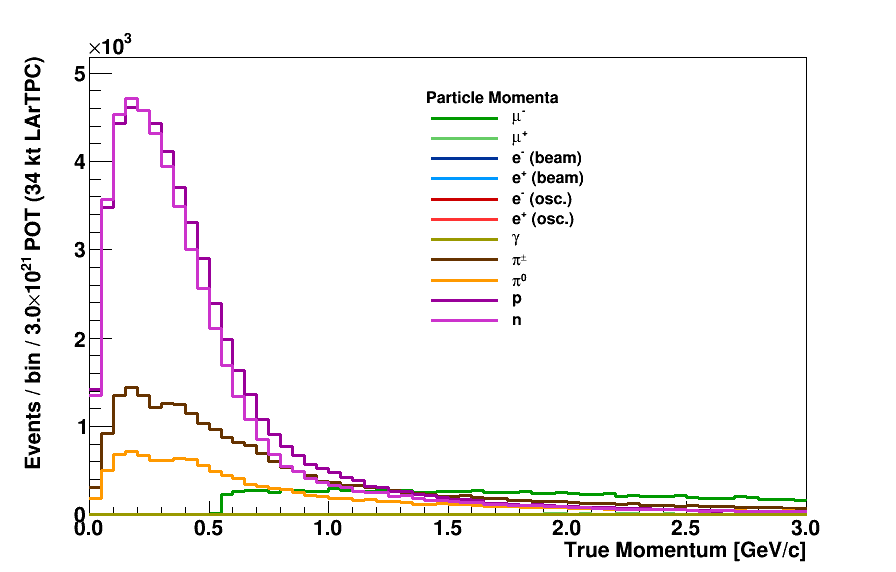
\includegraphics[scale=0.4]{figures/True_Momenta_per_Particle}
\label{fig:particle_momenta}
  \caption{Particle momenta distributions for particles coming from all fluxes ($\nu_e$, $\nu_\mu$, $\bar \nu_e$ and $\bar \nu_\mu$) at both near and far detector locations.  }
\end{figure}


\begin{figure}[h!]
  \centering
\includegraphics[scale=0.4]{figures/True_Theta_per_Particle}
\label{fig:particle_theta}
  \caption{Particle angle wrt to the beam axis distributions for particles coming from all fluxes ($\nu_e$, $\nu_\mu$, $\bar \nu_e$ and $\bar \nu_\mu$) at both near and far detector locations.  }
\end{figure}

\newpage


\begin{figure}[htp]
  \centering
  \label{fig:containment}
  
  \begin{tabular}{ccc}
    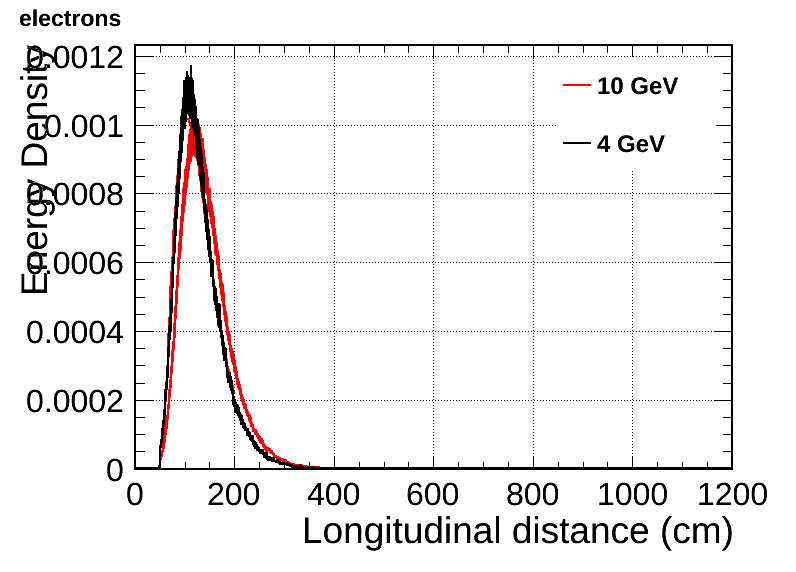
\includegraphics[scale=0.15]{figures/electrons_density_overlay}&
    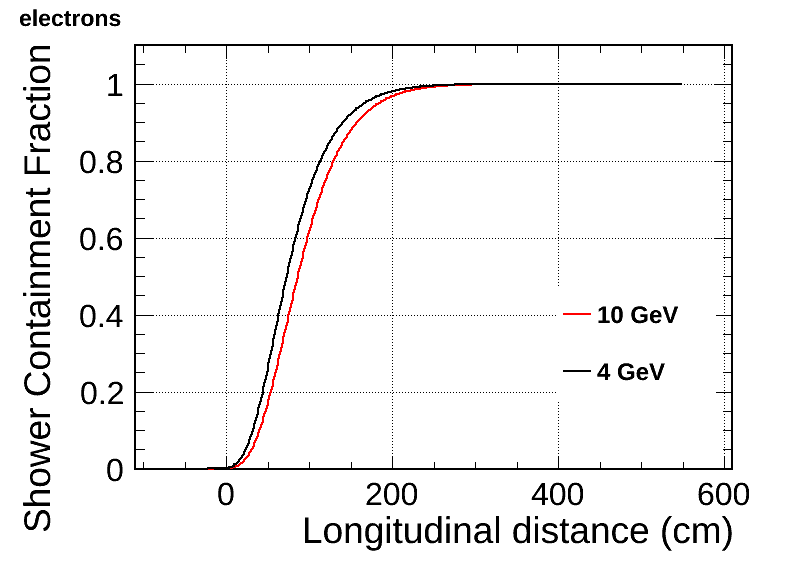
\includegraphics[scale=0.15]{figures/electrons_lcont_overlay}&
    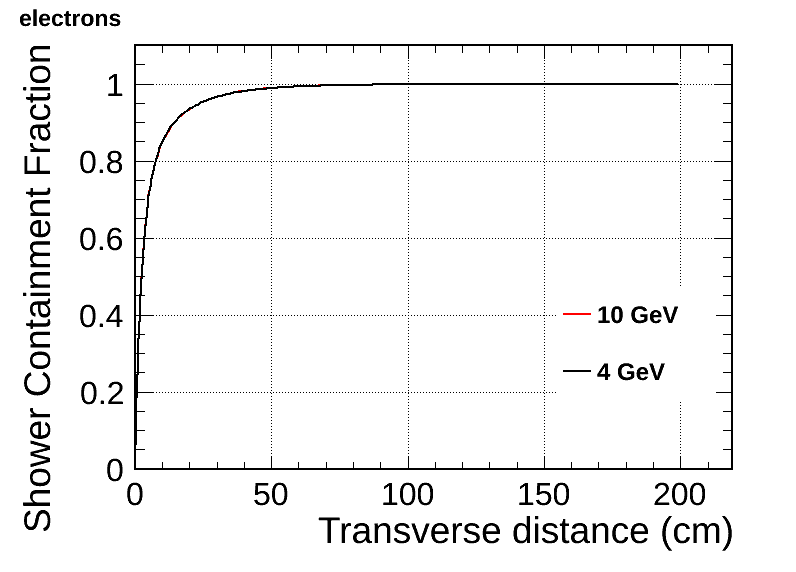
\includegraphics[scale=0.15]{figures/electrons_wcont_overlay}\\
 
 
    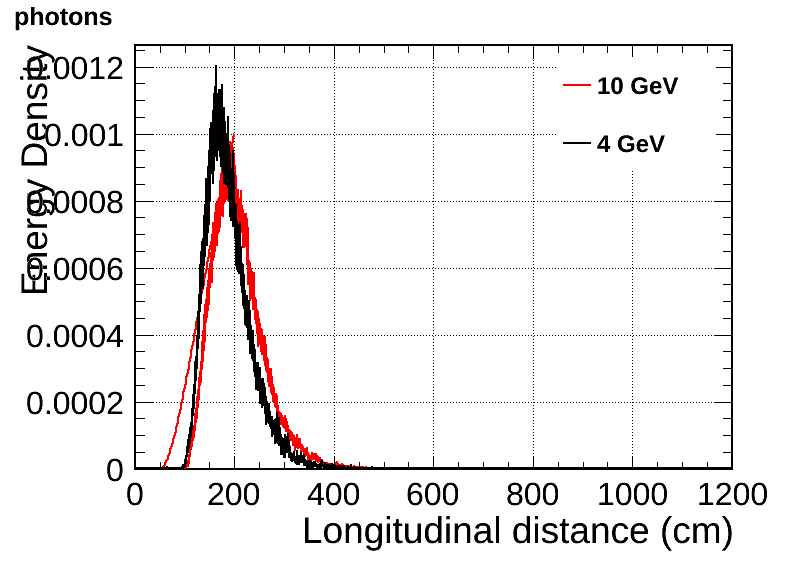
\includegraphics[scale=0.15]{figures/photons_density_overlay}&
    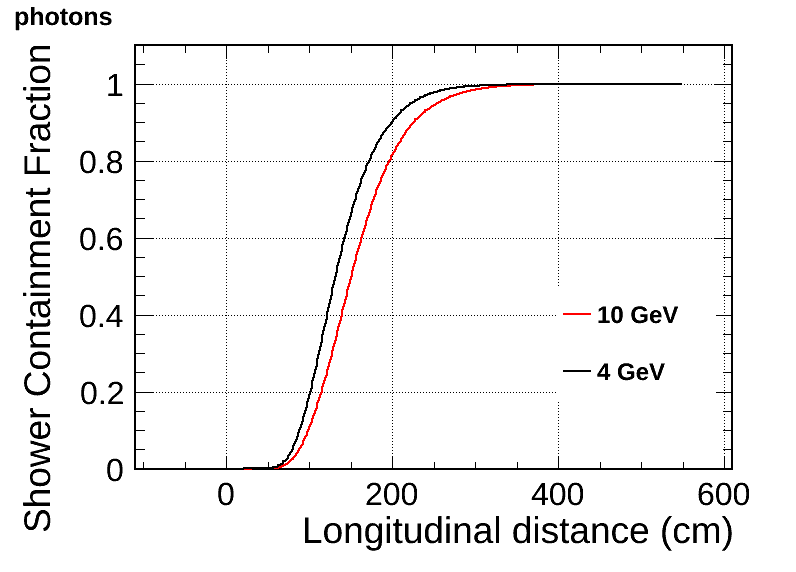
\includegraphics[scale=0.15]{figures/photons_lcont_overlay}&
    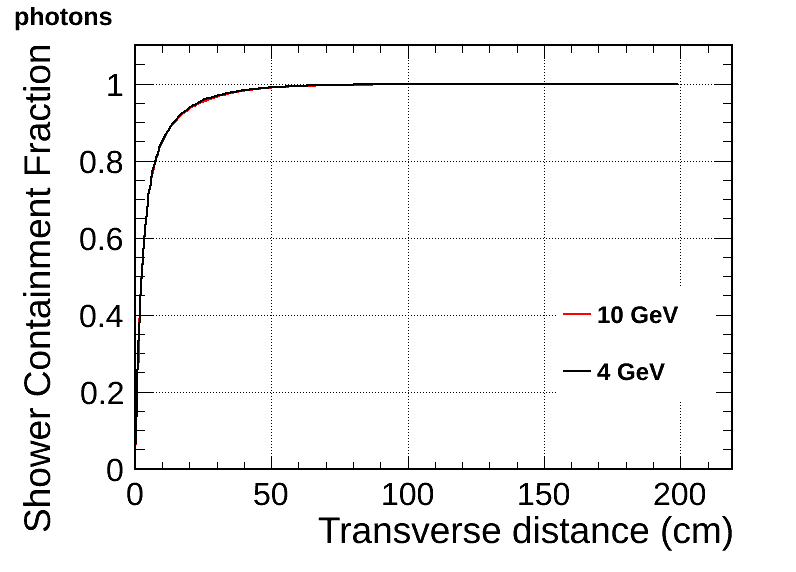
\includegraphics[scale=0.15]{figures/photons_wcont_overlay}\\
 

    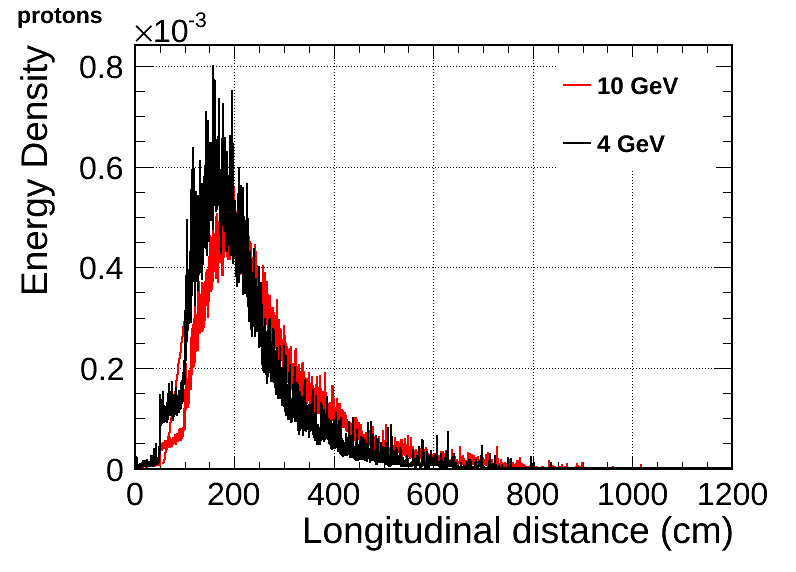
\includegraphics[scale=0.15]{figures/protons_density_overlay}&
    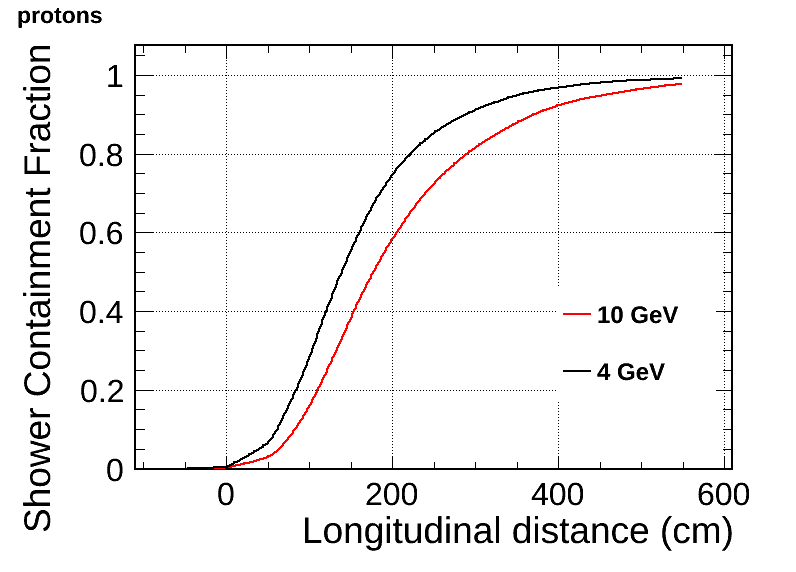
\includegraphics[scale=0.15]{figures/protons_lcont_overlay}&
    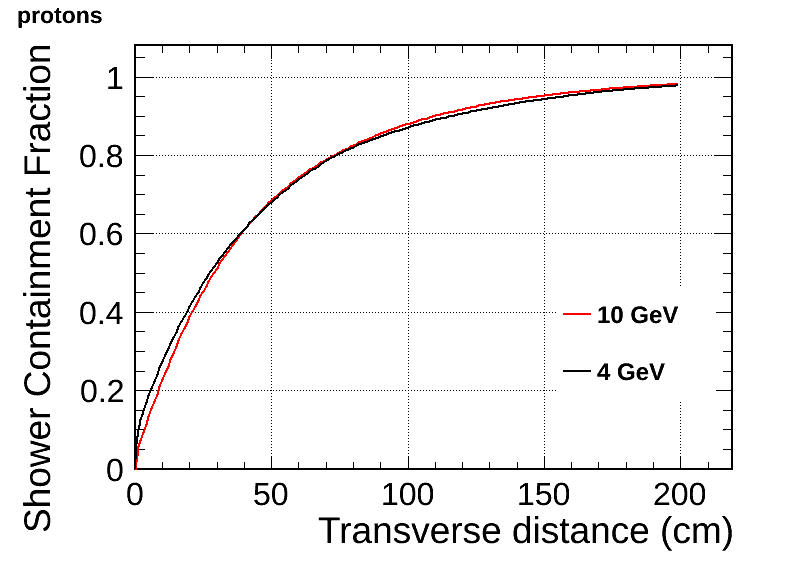
\includegraphics[scale=0.15]{figures/protons_wcont_overlay}\\
 
    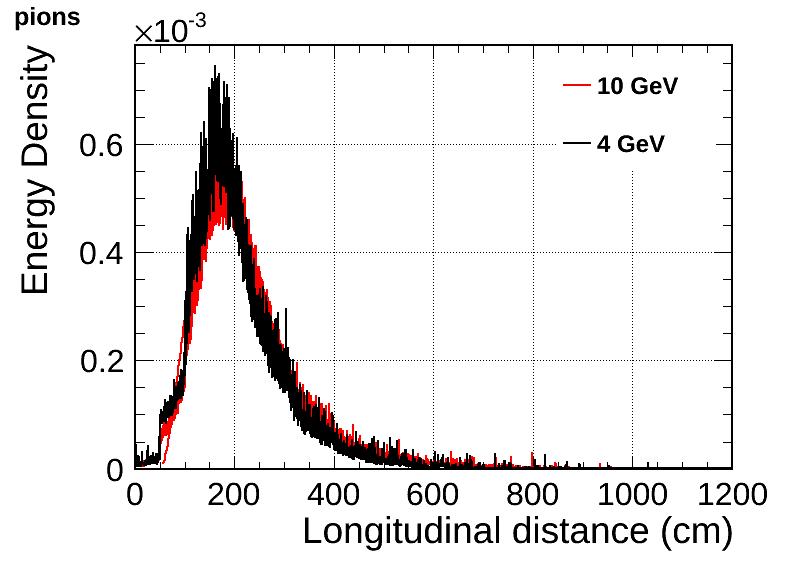
\includegraphics[scale=0.15]{figures/pions_density_overlay}&
    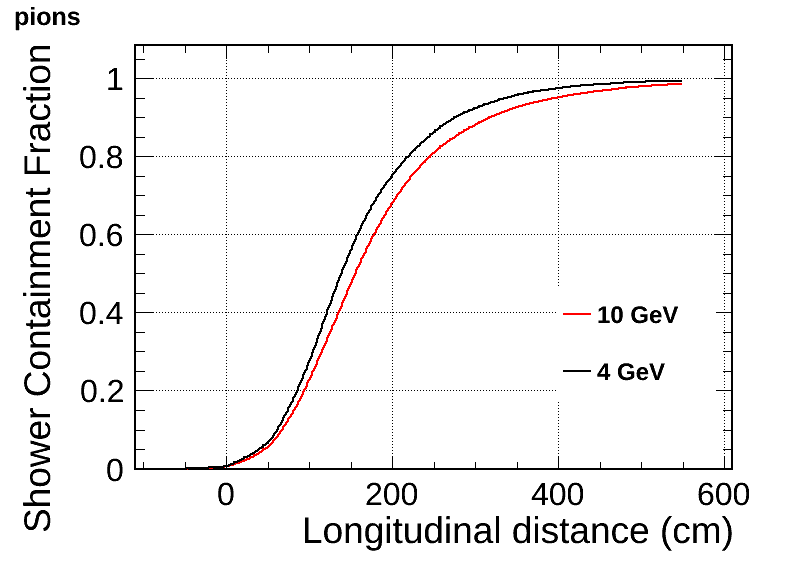
\includegraphics[scale=0.15]{figures/pions_lcont_overlay}&
    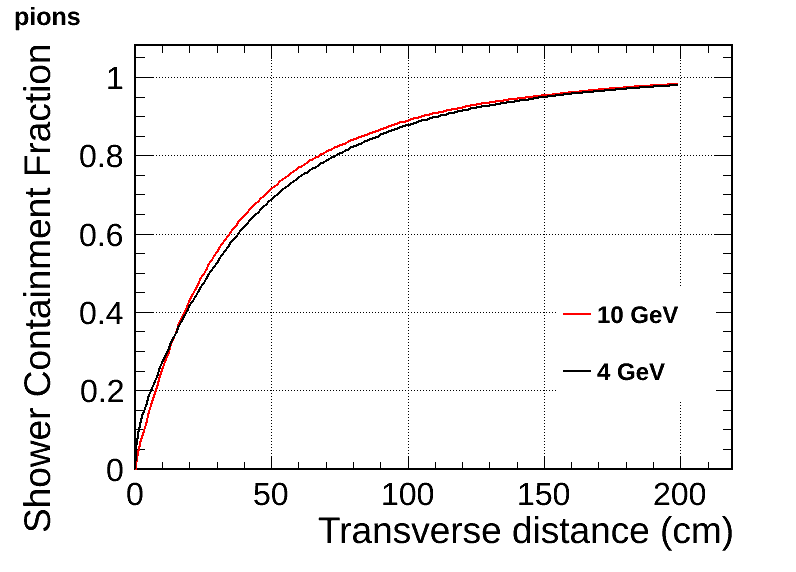
\includegraphics[scale=0.15]{figures/pions_wcont_overlay}\\
 
    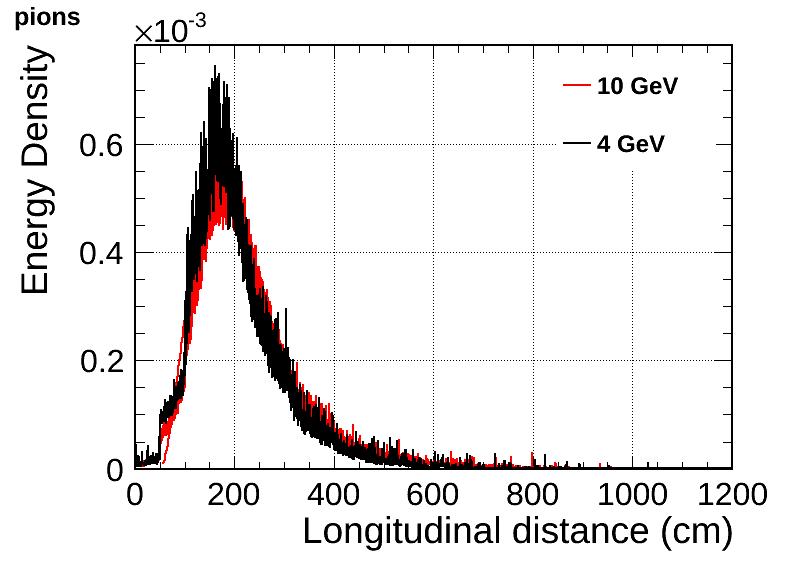
\includegraphics[scale=0.15]{figures/pions_density_overlay}&
    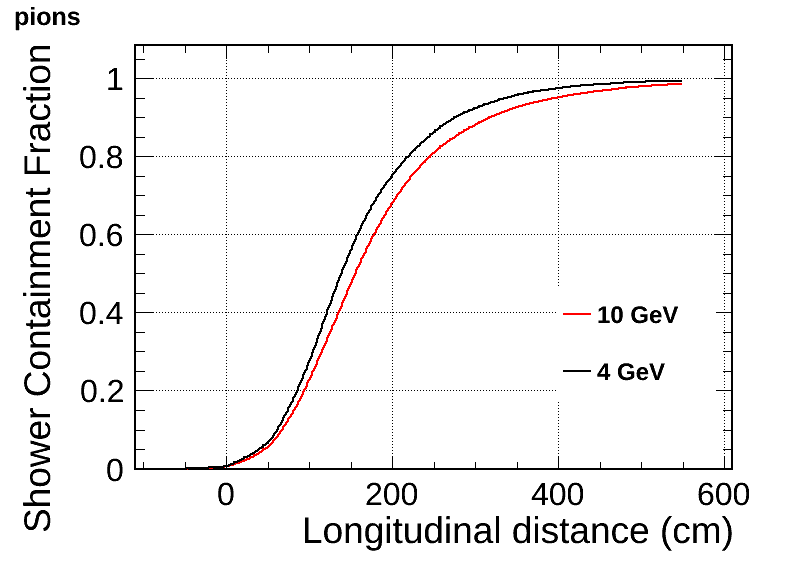
\includegraphics[scale=0.15]{figures/pions_lcont_overlay}&
    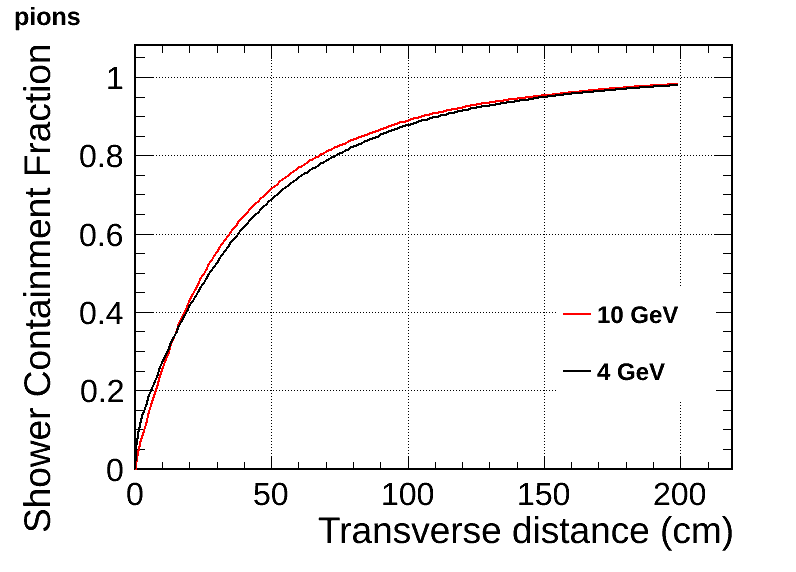
\includegraphics[scale=0.15]{figures/pions_wcont_overlay}\\
 
 
    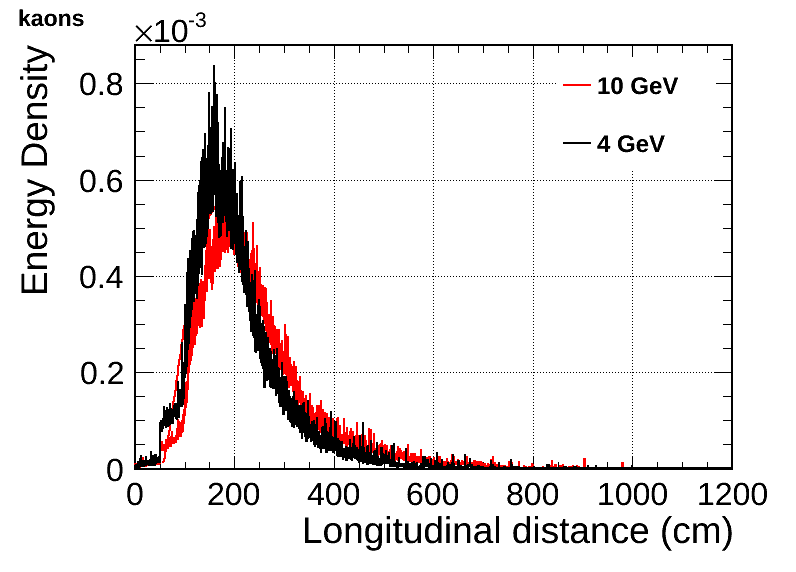
\includegraphics[scale=0.15]{figures/kaons_density_overlay}&
    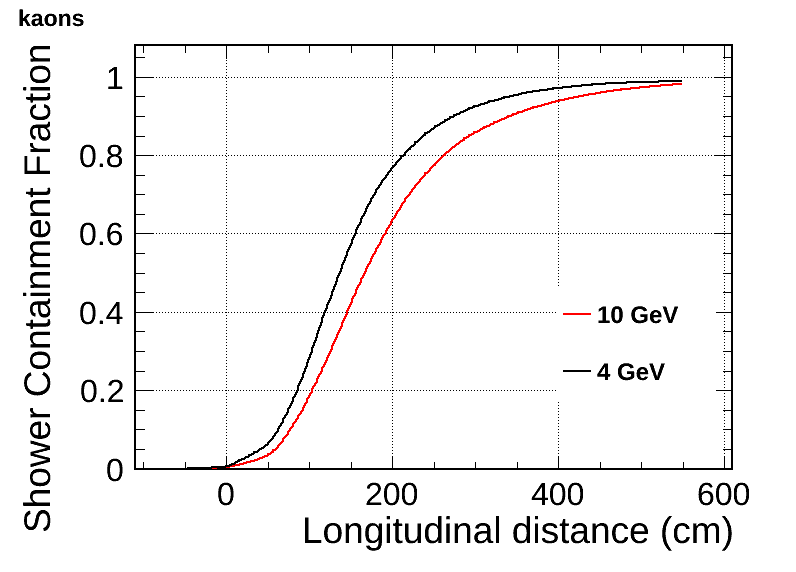
\includegraphics[scale=0.15]{figures/kaons_lcont_overlay}&
    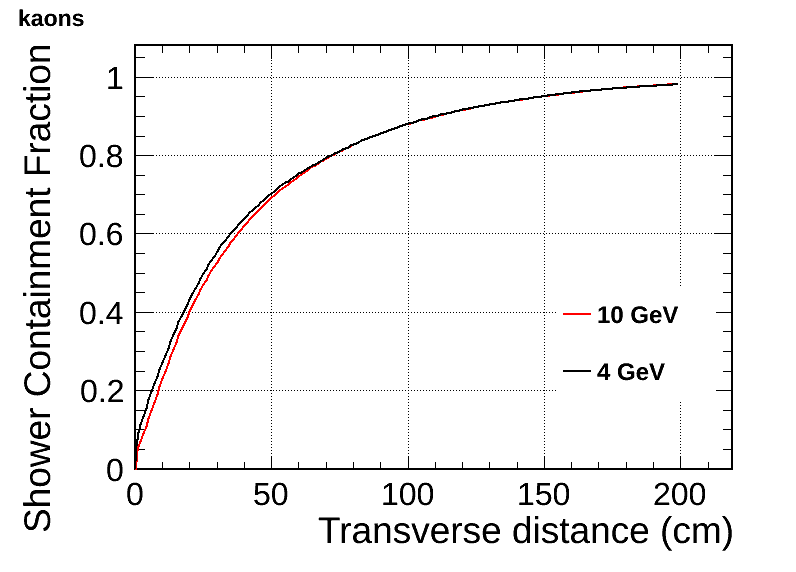
\includegraphics[scale=0.15]{figures/kaons_wcont_overlay}\\
 
  \end{tabular}
  \caption{Particle containment plots.}
\end{figure}

\clearpage
\subsubsection{Particle rates}
Estimation of  beam particles rates  necessary to collect high enough statistics in a reasonable time to obtain goals of of the measurements.
\subsubsection {Run plan}
Based of the rates from the beam and required rates from the physics considerations.



\subsection{Detector performance tests}

\subsubsection{Bethe-Bloch parametrisation of charged particles}

The SPCP will allow to study the detector response to charge particles from the test beam and will serve as a calibration detector. The measured energy deposition for various particles and its dependence on the direction of the particle will feed into our Monte Carlo generator and allow more precise reconstruction of neutrino energy and interactions topologies with good particle identifications.
 
{\bf How we compare with Lariat?} 
{\bf Multiple scattering}  

The set of single-phase prototype detector helped to understand the detector response to cosmic muons. But there is still lots to learn with additional studies. 
The charge  particle identification efficiencies  has been mapped for only limited range of the particle energies.  

\subsubsection{e/$\gamma$ separation}

The separation of the electrons from photons is the most important feature of the LAr TPC detectors for the search of the CP violation phase where we look for appearance of the $\nu_e$ in the $\nu_\mu$ beam.  Showers from electrons are part of the signal whilst the single photons might contribute to the background sample. The photons can undergo two process: pair production and Compton scattering. The dominant process for photons with energies of several hundreds MeV  is the e$^+$ e$^-$ pair production, but Compton scattering also occur at this energies. For pair production the e/$\gamma$ separation is achieved by looking at the beginning of the electromagnetic shower, where for election we see energy deposition typical for single MIP and for photon we see energy deposition consisted with two MIP. The separation of e/$\gamma$ has been measured in the ArgoNEUT experiment using neutrino scattering data with low statistics. Currently the separation efficiency is estimated to be at the level of of 94 \% (? cite and check the number). In case of the Compton scattering the off atomic electron the signal is much more difficult to distinguish from the electron from the CC $\nu_e$ scattering.

The separation of  the e/$\gamma$ measured by ArgoNEUT is not sufficient for the ELBNF experiment. Here we propose a measurement of the separation efficiency  as the function of energy and angle.  {\bf we need someone to look into this}



\subsubsection{Reconstruction efficiencies and particle identification}

The reconstruction of events in the LAr TPC is still a challenge but rapid progress has been achieved in recent years (cite pandora and other reconstruction algorithms). Despite the progress reconstruction algorithms have to rely Monte Carlo predictions which don't simulate liquid argon detectors responses correctly. Reconstruction algorithms will benefit greatly from test beam data particularly from the full scale prototype. The reconstruction algorithms will be trained to correctly reconstruct track, electromagnetic and hadronic showers.

The data of tracks and showers can be used to create a library which can be used for matching with he neutrino data, similar to the  LEM (library event matching).


Main issues for the reconstruction algorithms:
\begin{itemize}
\item The reconstruction algorithms try to use all three planes on the signal readout. if the orientation of the track/shower is such that it is aligned with wires on one of the plans it significantly reduces quality of reconstructed objects. 
\item Calorimetry with collection and induction planes. In the ICARUS experiment the deposited energy was reconstructed from the signal on the collection plane. The induction planes bipolar signal wasn't "stable" enough to use it for calorimetric measurement. In the ELBNF design there is additional shielding  wire plane which will improve the quality of the bipolar signal and the  test beam experiment will help with its calibration.
\item   Vertexing.
\item Reconstruction efficiency for low energy particles. The reconstruction algorithm suffer from the lose of fefficiency for low energy particle or particles which leave less than 200-300 hits. Training the algorithms on a low energy particles from the test beam will improve the quality and efficiency of the reconstructed objects.
\end{itemize}



\subsubsection{Cross section measurements}
Precise measurement of the  absorption and charge exchange of pions and kaons. Pion absorption is a large part of the pion nucleon cross section from 50 MeV to 500MeV with no data above about 1GeV pion kinetic energy. 
{\bf Add plots and values for known cross sections wit errors} 
\begin{itemize}
\item pion absorption on argon - Kotlinski, EPJ 9, 537 (2000)
\item pion cross section as a function of A - Gianelli PRC 61, 054615 (2000)
\end{itemize}
There is not currently a satisfactory theory describing absorption. The Valencia group (Vicente-Vacus NPA 568, 855 (1994)) developed model of    the pion-nucleus reaction with fairly good agreement, although not in detail. The actual  mechanism of multi-nucleon absorption
 is not well understood. 
 
\subsubsection{Charge sign determination}
It is not possible to determine charge of the particle on the event by event basis with non-magnetised LAr TPC detectors. However, the statistical analyst will be possible. We will fit the muon's half time which is different for muons and antimony due to different muon capture cross sections. For the $\mu^+$ for argon we expect about xx\% to be captured and for $\mu^-$ about yy\%. 

\subsubsection{Single track calibration}

\subsubsection{Shower calibration}

Reconstruction of neutrino energy depends of a quality of reconstruction of both electromagnetic and hadronic showers. 

- {\bf features of Hadronic shower in LAr TPC}
- {\bf features of electromagnetic shower in LAr TPC}
- Missing energy from neutral (Neutrons scattering)
 

\subsection{Other measurements} 
\subsubsection{Anti-proton annihilation }
\subsubsection{Proton decay background (cosmogenic $K^{0} \to K^+$)}




	

%\section{Single Phase LAr Detector [$\sim$10 pages; {\color{red} J. Stewart et al.}]}
\section{Single Phase LAr Detector} 
%\rm

	\subsection{LBNF detector}
Description of LBNF far detector components
\begin{itemize}
\item Overview of the far detector option
\begin{itemize}
\item List major components
\end{itemize}
\item Dimensions
\item Need for Modularity
\item Scaling from previous detectors
\item Possible development paths
\item Parameter summary
\end{itemize}


\subsection{CERN prototype detector}
Detailed description of CERN prototype detector components
\begin{itemize}
\item Overview of the CERN test Detector
\item Parameters table
\item Requirements (data rate, dimensions, gap to wall,  ?)
\item Installation
\end{itemize}

\subsubsection{APA}
\begin{itemize}
\item General description of the APA
\item Justification for the basic design (Dimensions, wire Wrapping, wire pitch and angle, hung nature)
\item Description of construction technique
\end{itemize}

\subsubsection{CPA and Field Cage}
\begin{itemize}
\item General description of the CPA - material, HV coupling, Stored energy, ….
\item Description of construction and installation
\item General description of the field cage
\item Description of design alternatives and engineering plan
\item Overview of design and installation plan
\end{itemize}

\subsubsection{TPC Readout}
A single APA has 2560 sense wires that need to be readout.  In order to  minimizing the capacitance, the preamplier noise, and the number of penetrations through the cryostat, the front-end (FE) electronics boards of the {\bf TPC electronics} are mounted in the cryostat on one end of the wire frame just outside of the active TPC volume.  A single APA is readout by 20 sets of FE readout boards with each FE reading in 128 wire channel inputs (40 U-view + 40 V-view + 48 X-view) and each FE transmitting 4 outputs through the cryostat to back-end electronics.
 
The present design has a maximum wire length of 7.3~m (induction planes)
with a corresponding capacitance of 164~pF and an expected intrinsic noise of 400 electrons.
The preamplifiers include shaping circuits, and are implemented in 16 channel FE ASICs, which couple directly to 16 channel, 12 bit ADC ASICs operating at 2~MS/s, which include a 1:8 multiplexing stage.
The ADCs are read out by a commercial FPGA, which provides an additional factor of 4 in multiplexing.
This level of multiplexing is low enough for transmitting the entire raw data stream,
while also being high enough that the number of signal lines is actually smaller than the number of the various
power and control lines, and therefore easily manageble by a small number of feedthroughs.
Neither zero suppression nor data compression is implemented at the level of the cold readout electronics.
Not only does this greatly simplify the cold electronics design,
but it also automatically satisfies the requirement that the system be capable of such raw readout.
The FPGAs transmit the data via high-speed (1~Gbps) serial links to the DAQ system.
For the final detector it is expected that a dedicated digital control and data transmission ASIC (COLDATA) will be developed which
replaces the commercial FPGA.
While the COLDATA is well under way, it is not expected to be available in time for the CERN test,
which will instead make use of the proven FPGA technology.
While serious doubts regarding the longevity of commercially-available FPGAs at LAr temperatures strongly argues against
their use in the Far Detector, where reliability over 15-20 years is required,
this is not a concern for the CERN test, where the proven FPGA lifetime of at least a year is adequate.

The front end electronics is organized as a stack of three boards comprising the Cold Mother Board assembly (CMB),
which mounts directly on the APA.
First is the Analog Mother Board, on which are mounted the FE and ADC ASICs.
Second and third are the FPGA and SERDES Mezzanine Boards, themselves mounted on the Analog Mother Board.
Each CMB has eight sets of FE and ADC ASICs and instruments 128 wires.
A Faraday cage (FC) covers the end of the APAs to shield the electronics from ambient noise.
The FC also serves to prevent any Ar gas-bubbles from LAr boiled by the electronics' heat from entering the active TPC volume.
Figure \ref{fig:coldelec} shows a schematic of the cold electronics. 

\begin{figure}[htb]
\centering
\begin{minipage}[b]{1.0\textwidth}
\begin{center}
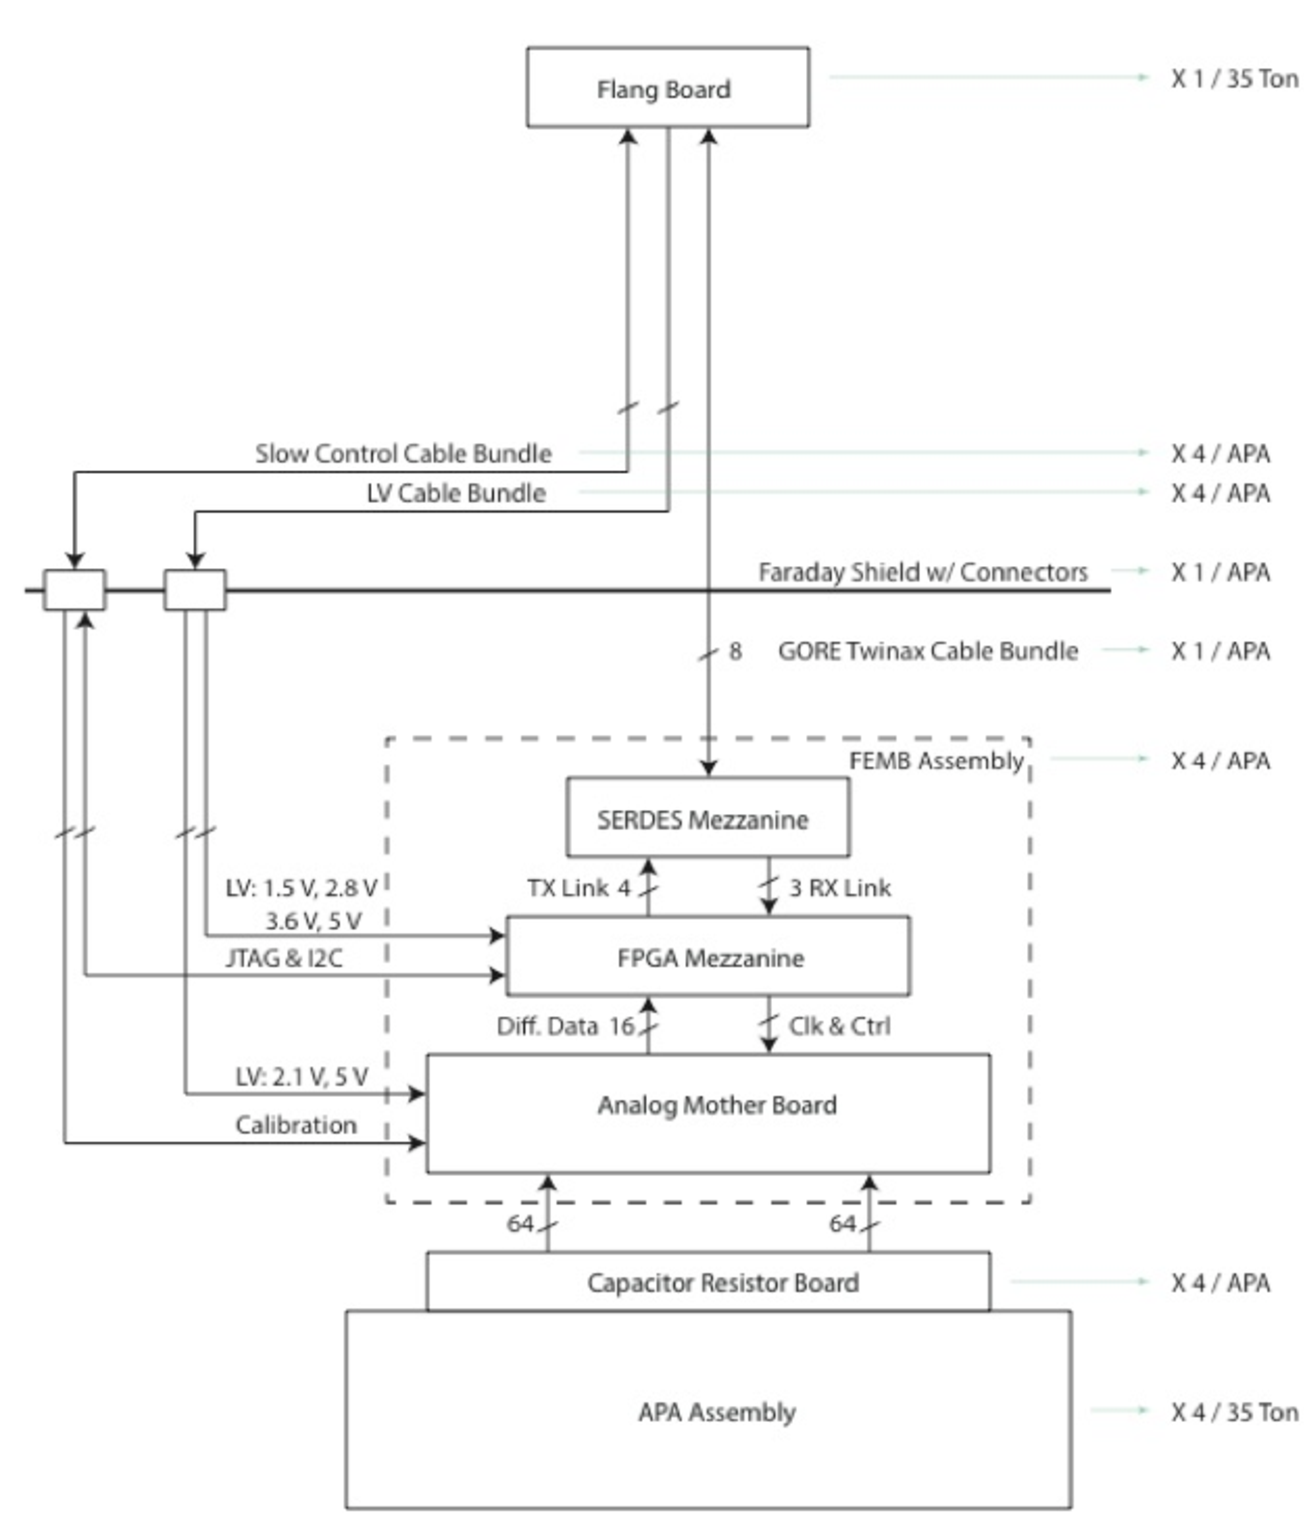
\includegraphics[width=.75\textwidth]{figures/fe-electronics-block-diagram.pdf}
\end{center}
\end{minipage}
\caption{Layout of the TPC cold from end (FE) electronics..}
\label{fig:coldelec}
\end{figure}


Besides the high-speed signal cable, which is a twin-axial cable bundle manufactured by GORE,
there are cable bundles for low-voltage power, wire-bias voltages, and various slow controls and monitoring.
The  cable bundles will be connected through a feedthrough on the roof of the cryostat. 


\begin{figure}[htb]
\centering
\begin{minipage}[b]{1.0\textwidth}
\begin{center}
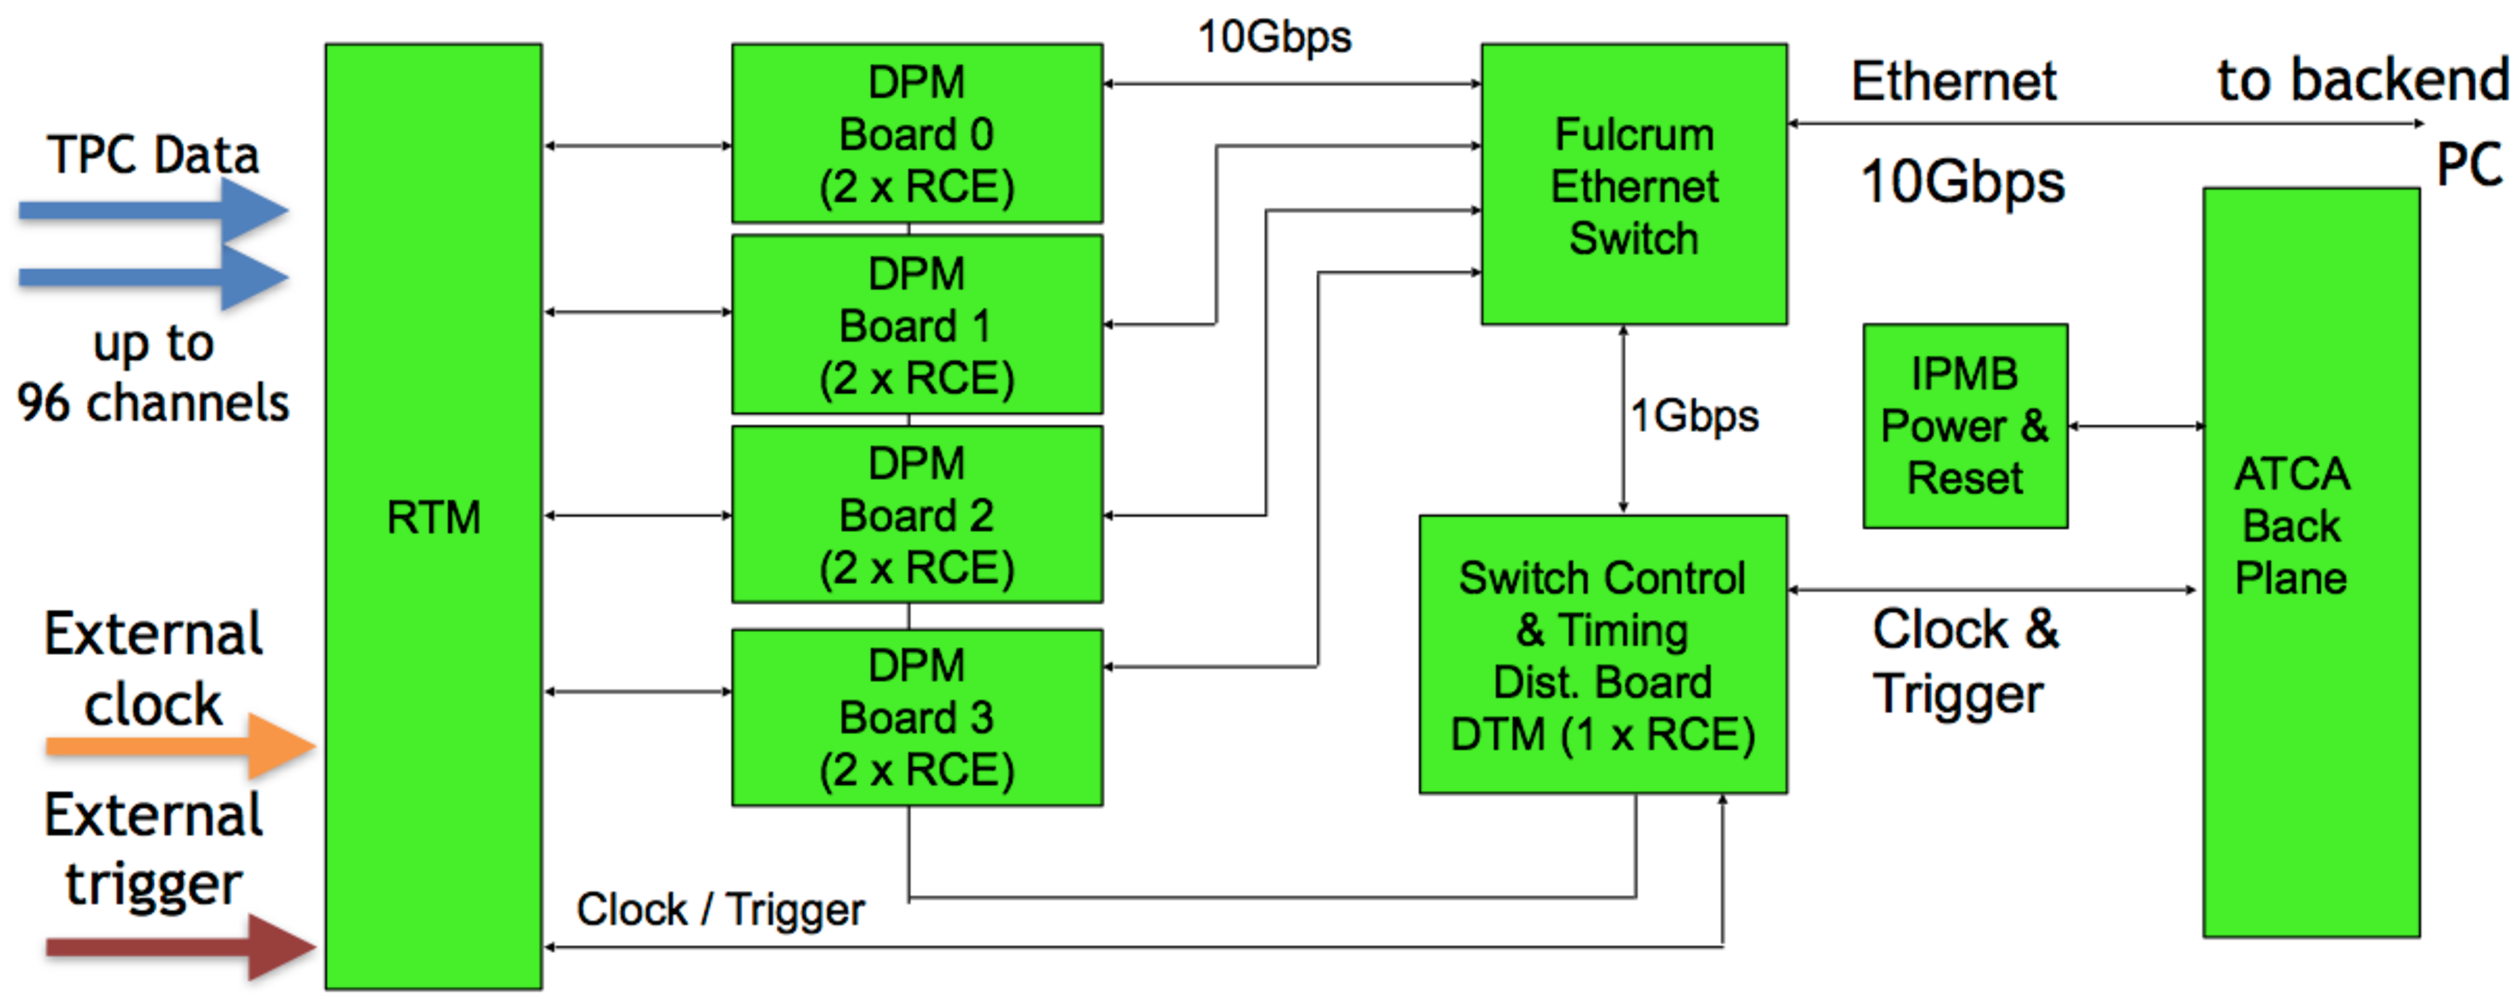
\includegraphics[width=1.0\textwidth]{figures/rce-block.pdf}
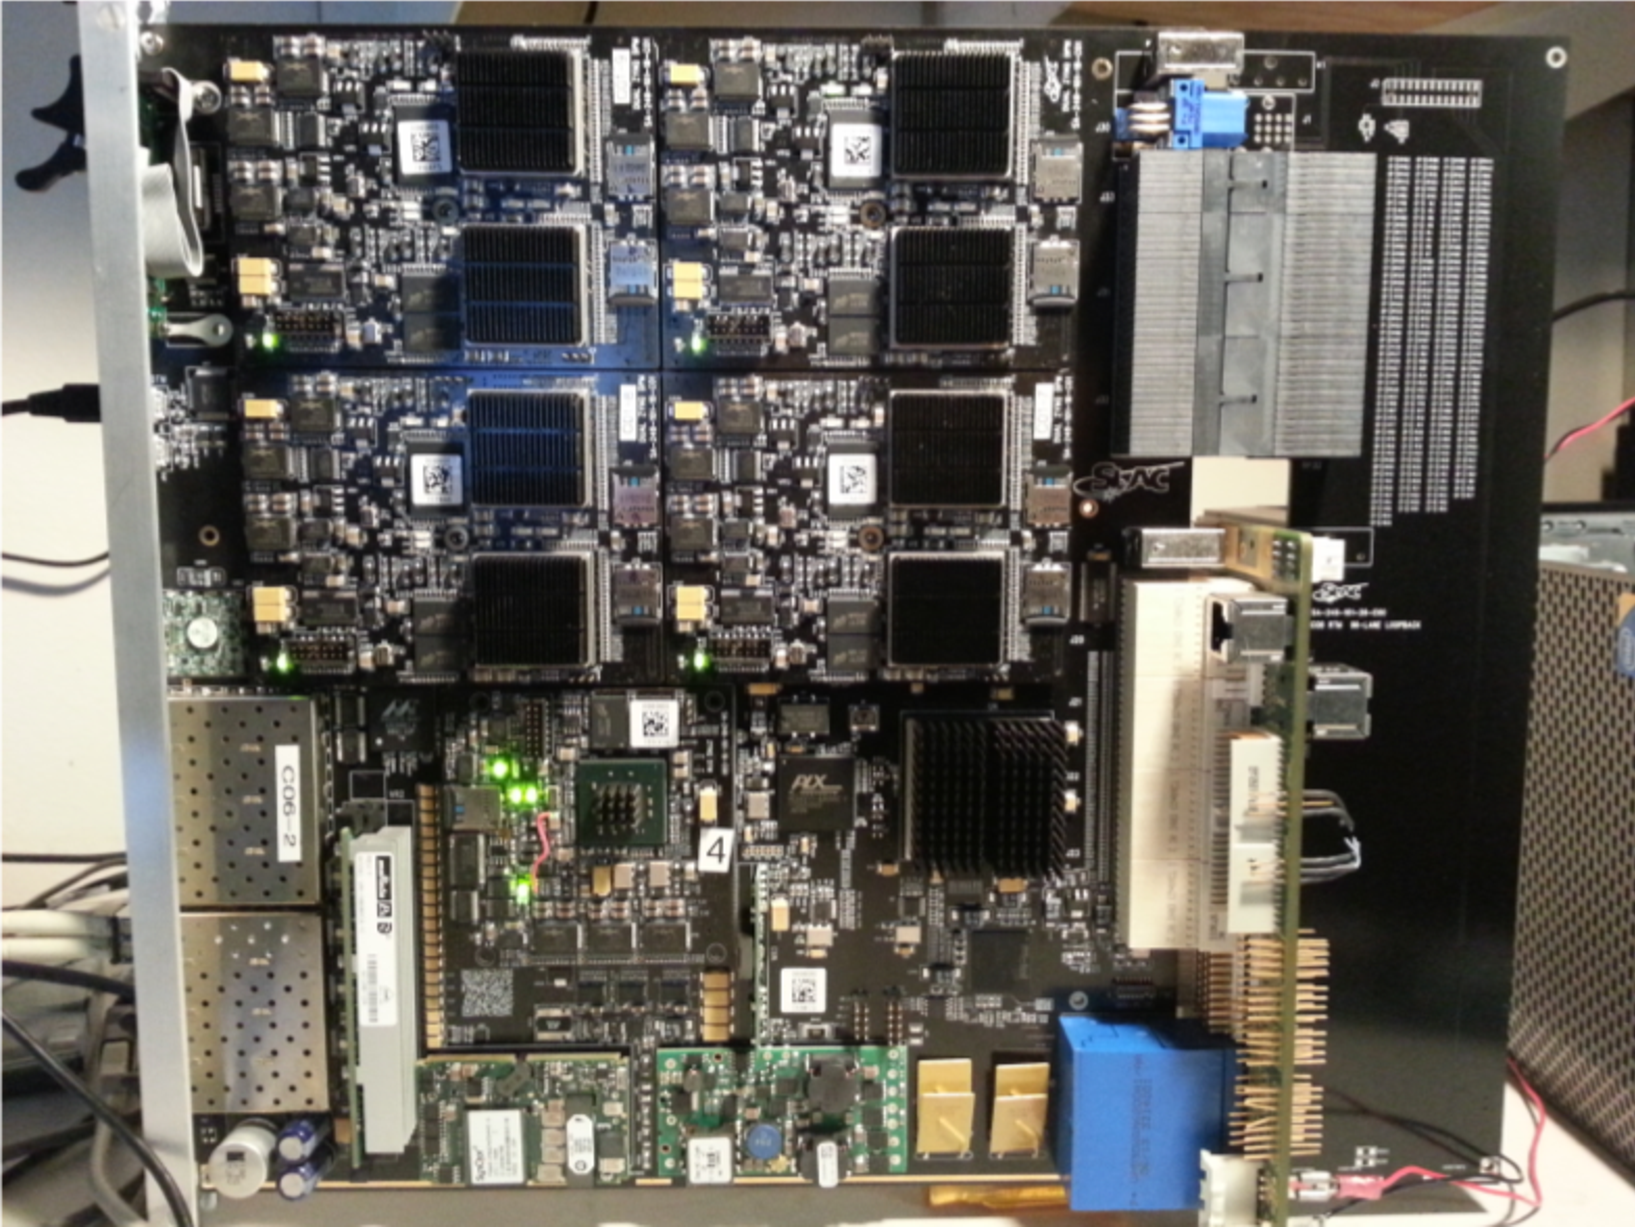
\includegraphics[width=.5\textwidth]{figures/COB-gen3.pdf}
\end{center}
\end{minipage}
\caption{Top: Schematic for the TPC DAQ system. Bottom: The COB (left of the large connectors) and RTM (right).}
\label{fig:rce}
\end{figure}

The primary interface between the TPC front-end electronics (FE) and the DAQ subsystem consists of an ATCA-based system of
RCEs (Reconfigurable Cluster Elements).
The RCE system receives the serialized raw data for the FE, performs zero-suppression on it,
and packetizes and transmits the resulting sparsified data to a back-end data farm for event building and further processing.
Additionally, the RCE system transmits timing and control signals to the FE as well as forwarding configuration data
to them at start-up.     

The RCE system consists of the following components:
a commercial ATCA shelf (2-, 6-, or 14-slot), a Cluster-On-Board (COB) which is the "front board" in ATCA terms,
and a Rear-Transition-Module (RTM) which is the "rear board".
A schematic of the system is shown in Figure \ref{fig:rce}.
The COB is a custom board, developed by SLAC, which holds the processing power of the system.
The COB (see Figure \ref{fig:rce}) consists of 5 bays for holding daughter boards, an onboard 10-GbE switch,
and both 10- and 1-Gb ethernet connections for communications with the back-end system.
Four of the daughter-board bays are for Data Processing Modules (DPM), each of which can hold up to two RCEs.
The RCE is the core procession unit of the system; it is made up of a modern SoC (currently, the Xilinx Zynq-7045)
with multiple high-speed I/O ports (up to 10-Gbps each) and external DRAM and flash memory controllers.
The other bay on the COB contains the Data Transmission Module (DTM) which is responsible
for distributing timing and trigger information to and between the DPMs.  

While the COB hardware is application agnostic, the RTM is application specific.
The RTM provides the mechanical interface between the front-end (or, in our case, the flange electronics)
and the back-end, as well as other external sources such as the timing or trigger systems.
In this case we will use fiber optic connections between the flange and the TPC DAQ using 8 12-channel (full duplex)
CXP connectors on the RTM. 

With the assumption that each cold FE board multiplexes it's 128 wire channels to 4 outputs at 1-Gbps each,
the non-zero suppressed data for 1 APA can be fed into a single COB (containing 8 RCEs).
Each RCE would receive data from 2 FE boards, perform zero-suppression, and send the result to the back-end.  \\


The {\bf PDS front-end electronics} resides outside of the cryostat in
instrumentation racks. A custom module for receiving SiPM signals has
been designed and built. The module also performs signal processing in
the front-end as preprocessing for trigger and DAQ.  The module is
called the SiPM Signal Processor (SSP) and consists of 12 readout
channels packaged in a self-contained 1U module.  Each channel
contains a fully-differential voltage amplifier and a 14-bit, 150-MSPS
analog-to-digital converter (ADC) that digitizes the waveforms
received from the SiPMs. There is no shaping of the signal, since the
SiPM response is slow enough relative to the speed of the digitization
to obtain several digitized samples of the leading edge of the pulse
for the determination of signal timing. Digitized data is processed by
a Xilinx Artix-7 Field-Programmable Gate Array (FPGA).  The use of the
FPGA processing allows for a significant amount of customization of
the SSP operation. \\

%The data streams from the TPC and the PDS will be merged and the concepts are being implemented and tested at the 35t detector.






\begin{itemize}
\item Overview of the TPC readout chain (include main parameters)
\item Overview of the cold electronics
\item Overview of the RCE and interface to the DAQ
\item	Discussion of sparsification and triggering
\end{itemize}

\subsubsection{Photon Detection System}
\begin{itemize}
\item General description of the photon system including requirements
\item Overview of the photon system alternatives and selection process
\item Description of the readout and development plans
\end{itemize}

\subsubsection{DAQ, Slow control and monitoring}
\include{DAQ}
\begin{itemize}
\item General description of the DAQ system
\item Plans and status for the 35t and next steps
\item Needs for a slow control system
\end{itemize}

\subsubsection{Offline requirements and software}






\section{Cryostat and Cryogenics system} % [$\sim$5 pages; {\color{red} David/Barry/Jack}]}
	
\subsection{Cryostat}

The Single Phase TPC test at CERN will use a membrane tank technology to contain  673 tons of LAr, equivalent to about $483 m^3$. The design is based on a scaled up version of the LBNE 35-ton Prototype\cite{montanari_35ton} 
% (this is a comment) add \cite{montanari_sbn_perf} if public access in docdb 9270 (AH)
and the Fermilab Short-Baseline Near Detector\cite{acciarri_sbn_proposal}.  
The cryostat will use a steel outer supporting structure with a metal liner inside to isolate the insulation volume, similar to the one of the dual phase detector prototype WA105 $1\times1\times3$ and to the Fermilab Short-Baseline Near Detector. The support structure will rest on I-beams to allow for air circulation underneath in order to maintain the temperature within the allowable limits.
This section describes the proposed design, whose scope encompasses the following components:

\begin{itemize}
\item steel outer supporting structure,
\item main body of the membrane cryostat (sides and floor), 
\item top cap of the membrane cryostat.
\end{itemize}

A membrane cryostat design commonly used for liquefied natural gas (LNG) storage and transportation will be used. In this vessel a stainless steel membrane contains the liquid cryogen. The pressure loading of the liquid cryogen is transmitted through rigid foam insulation to the surrounding outer support structure, which provides external support. The membrane is corrugated to provide strain relief resulting from temperature related expansion and contraction. The vessel is completed with a top cap that uses the same technology.

Two membrane cryostat vendors are known: GTT (Gaztransport \& Technigaz) from France and IHI (Ishikawajima-Harima Heavy Industries) from Japan. Each one is technically capable of delivering a membrane cryostat that meets the design requirements for this detector. To provide clarity, only one vendor is represented in this document, GTT; this is for informational purposes only. Figure 1 shows a 3D model of the GTT membrane and insulation design.


\begin{figure}[htbp]
\begin{center}
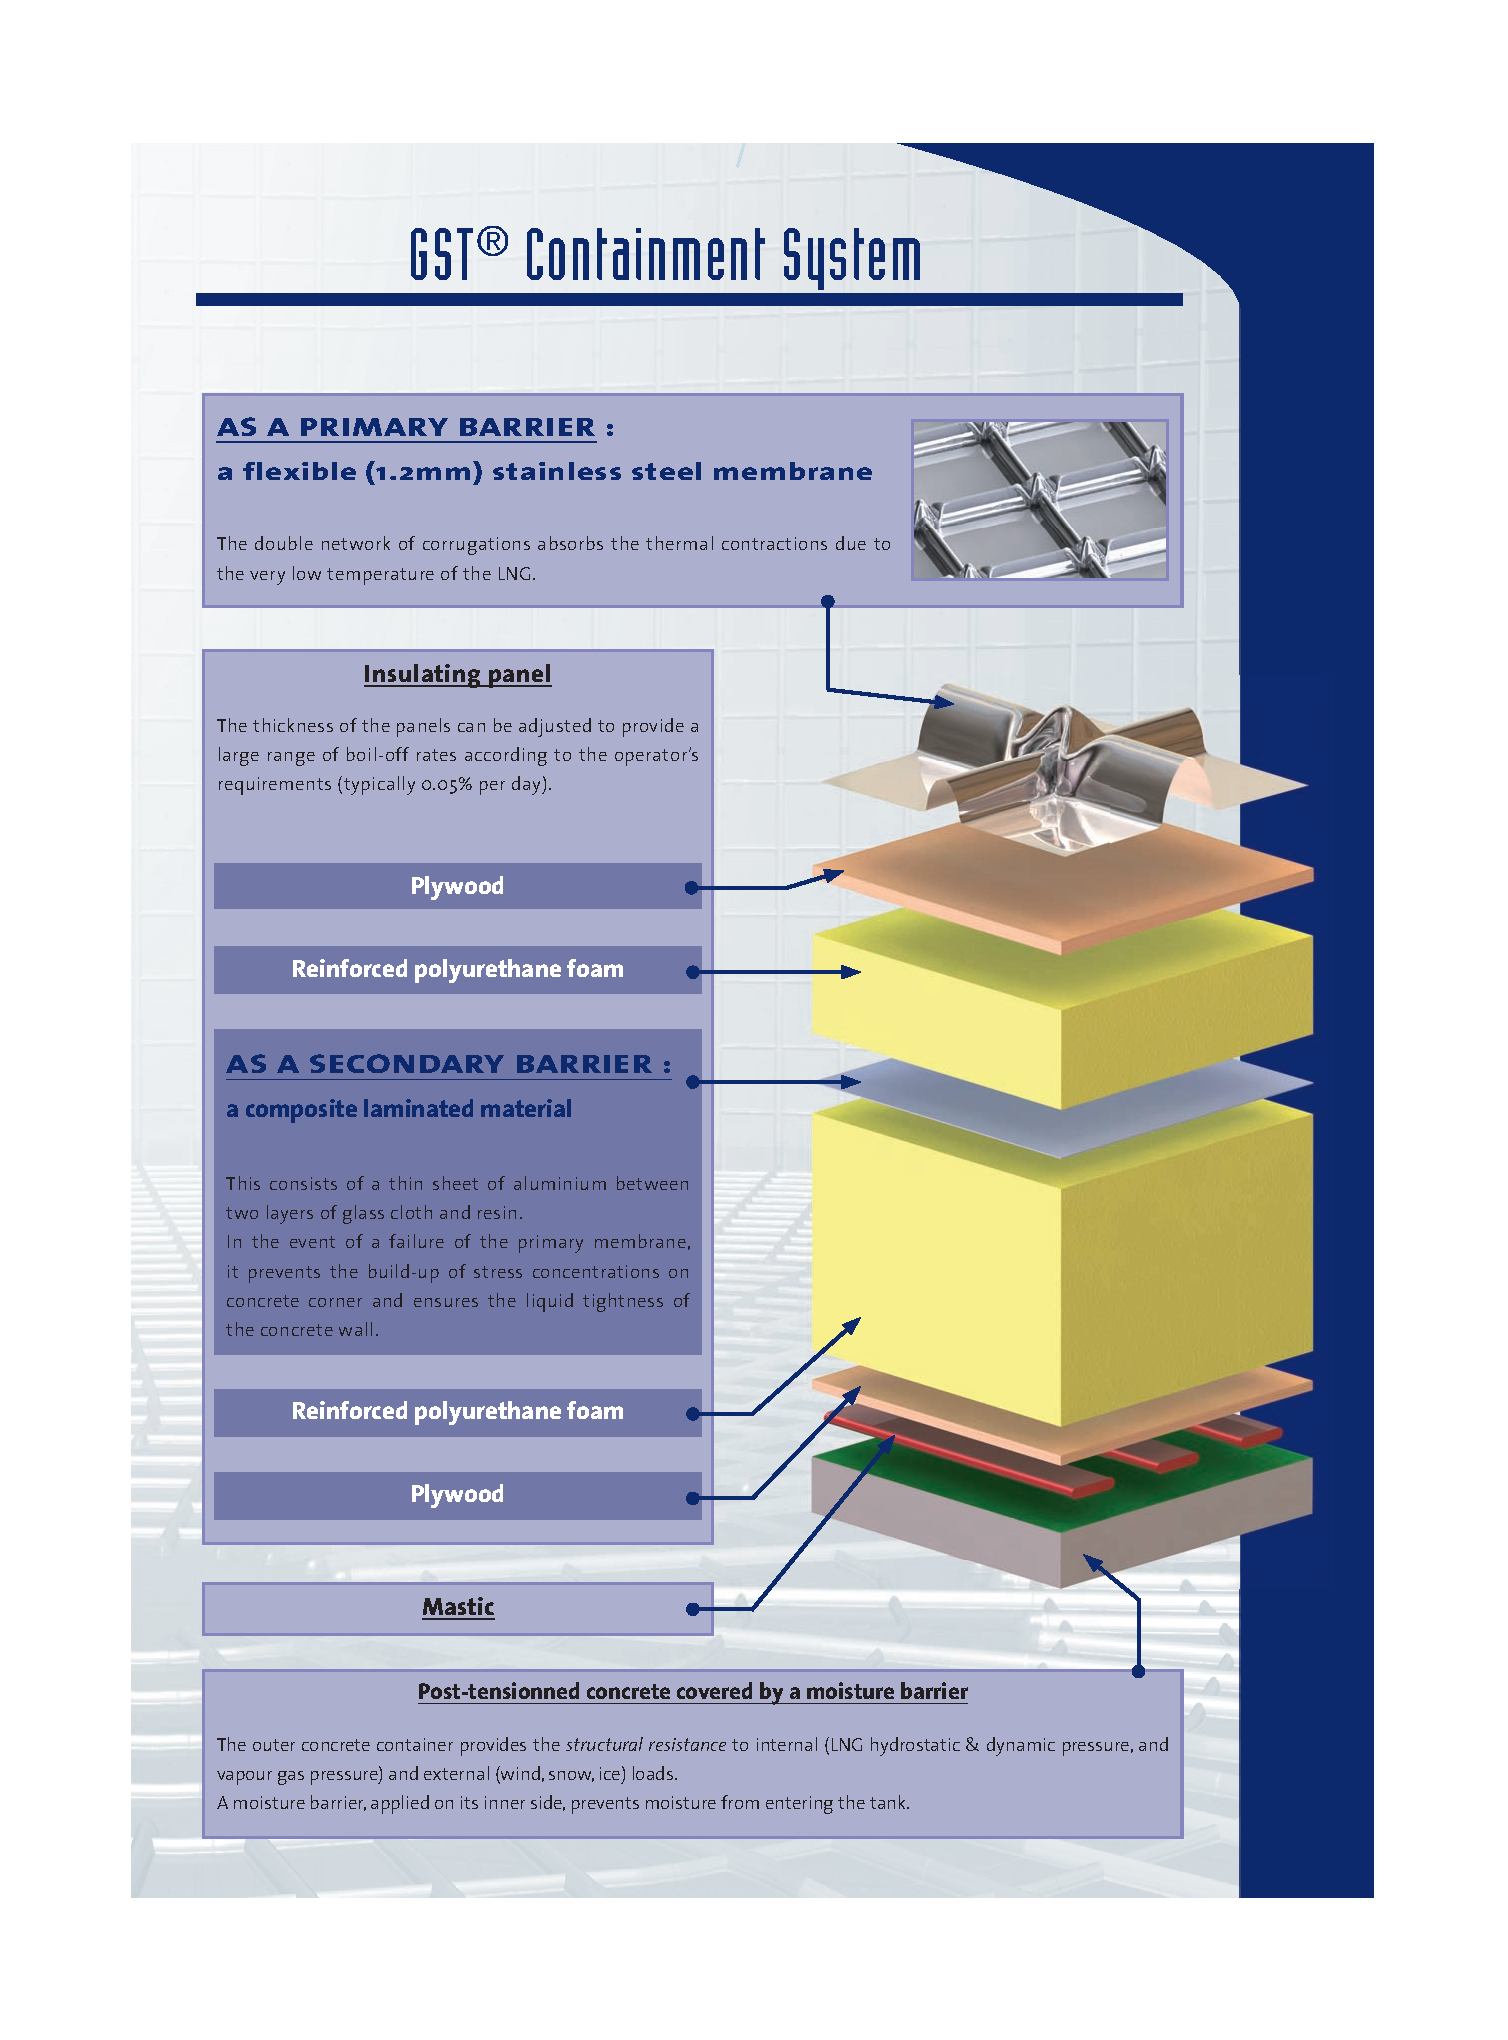
\includegraphics[width=.9\textwidth]{figures/membrane-exploded-view}
\caption[Exploded view of the membrane cryostat technology]{\label{fig:lar-org} Exploded view of the membrane cryostat technology}
\end{center}
\end{figure}

The conceptual proposed design for the Single Phase Test at CERN cryostat is a rectangular vessel measuring 8.8 m in length (parallel to the beam direction), 7.8 m in width, and 8.0 m in height; containing a total mass of 673 tons of liquid argon. Figure~\ref{fig:cryostat-views} shows side and end views of the cryostat respectively. Figure 15 shows a 3D view. To minimize the contamination from warm surfaces, during operation the temperature of all surfaces in the ullage shall be lower than 100 K. 
The top plate will contain two hatches for the installation of the TPCs; it will also contain a manhole to enter the tank after closing the hatches, and several penetrations for the cryogenic system and the detector. 

\begin{figure}
\begin{center}
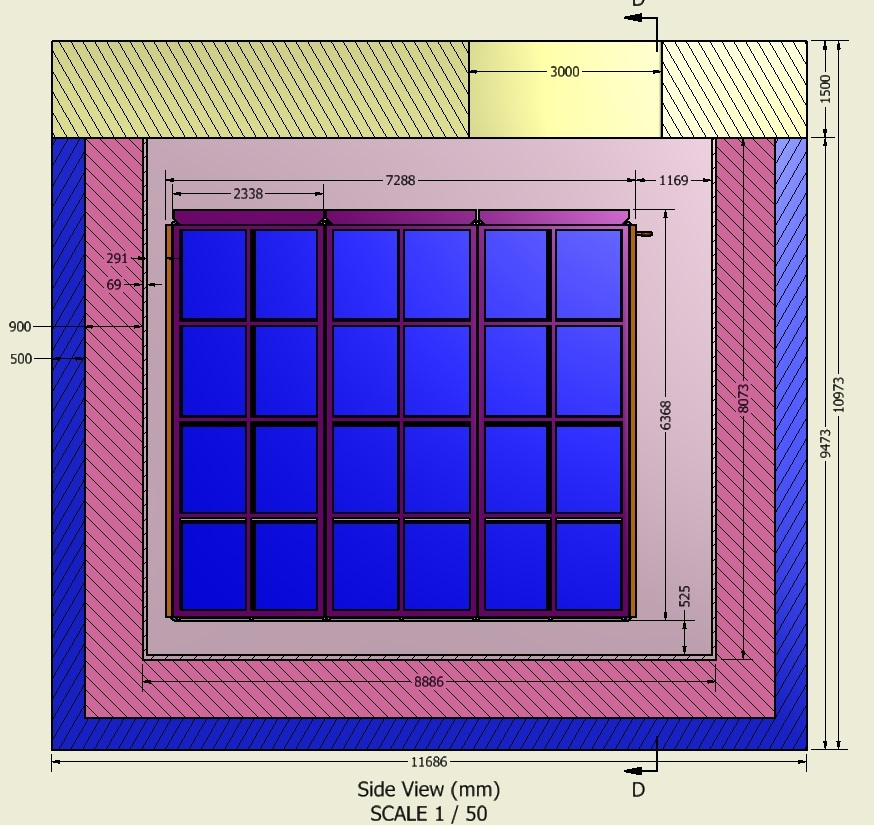
\includegraphics[width=.53\textwidth]{figures/cryostat-side-view} 
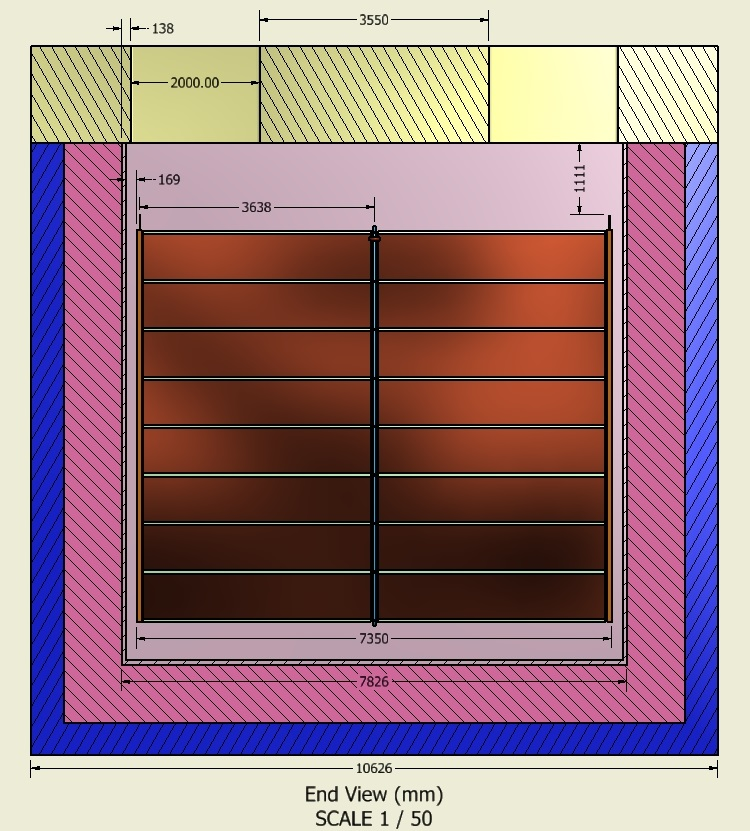
\includegraphics[width=.42\textwidth]{figures/cryostat-westend-view}  
\caption[Views of cryostat]{\label{fig:cryostat-views} Side (left) and end (right) views of cryostat}
\end{center}
\end{figure}

\begin{figure}[htb]
\begin{center}
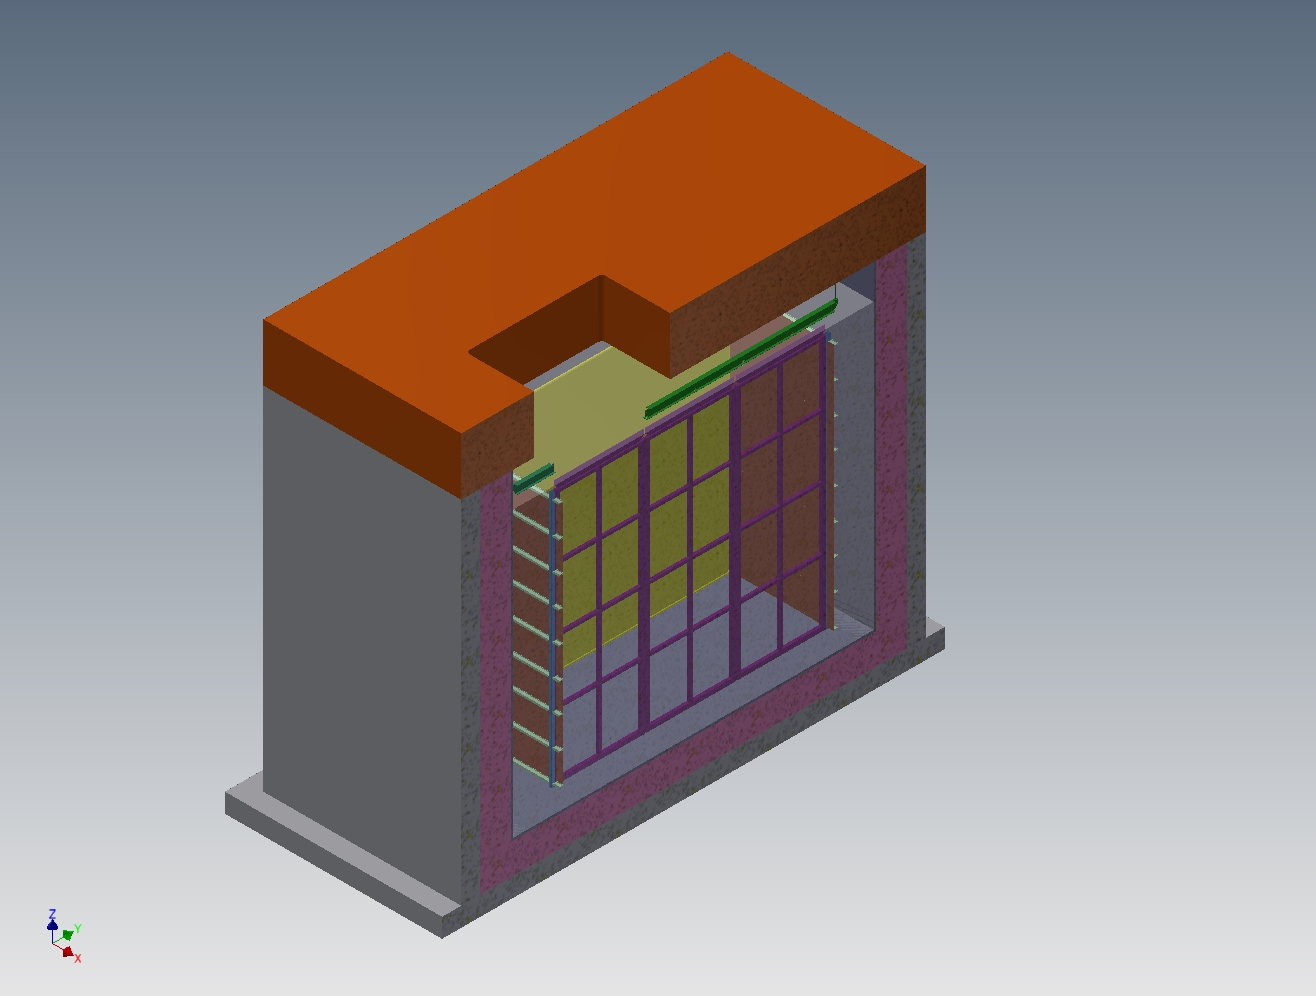
\includegraphics[width=.75\textwidth]{figures/cryostat-isometric-view} 
\caption[Isometric view of cryostat]{\label{fig:cryostat-views} Isometric view of the membrane cryostat}
\end{center}
\end{figure}

\textbf{Design Parameters}

This design includes technical solutions that may be of interested for the future needs of the Long Baseline Neutrino program. For example the use of a cold ullage (\textless  100 K) to lower the impurities in the gas region, and of a LAr pump outside the cryostat to minimize the effect of noise, vibration and microphonics to the TPC inside the liquid argon volume.

The design parameters for the TPC Test at CERN cryostat are listed in Table~\ref{tbl:cryogenics-design-parameters}.

\begin{table}[htpb]
\caption{Design requirements for the membrane cryostat}
\label{tbl:cryogenics-design-parameters}
\centering
\begin{tabular}{|p{.4\textwidth}|p{.5\textwidth}|}
\hline
\textbf{Design Parameter} & \textbf{Value} \\ \hline
Type of structure & Membrane cryostat \\ \hline
Membrane material    &  SS 304/304L, 316/316L or equivalent. \\ \hline
Fluid & Liquid argon (LAr)  \\ \hline
Other materials upon approval.\\ \hline
 Outside reinforcement (support structure)  &  Steel enclosure with metal liner to isolate the outside from the insulation space, standing on legs to allow for air circulation underneath. \\ \hline
 Total cryostat volume  &  538 m3 \\ \hline
 Total LAr volume  &  483 m3 \\ \hline
LAr total mass   & 673,000 kg  \\ \hline
Minimum inner dimensions (flat plate to flat plate).   &  7.8 m (W) x 8.8 m (L) x 8.4 0 (H) \\ \hline
Depth of LAr   &  7.2 m (0.82 m ullage, same as LBNF) \\ \hline
Primary membrane   &   1.2 mm thick SS 304L corrugated stainless steel\\ \hline
Secondary barrier system   &  GTT design; 0.07 mm thick aluminum between fiberglass cloth. Overall thickness 1 mm located between insulation layers.  \\ \hline
 Insulation  &  Polyurethane foam (0.9 m thick from preliminary calculations) \\ \hline
Maximum static heat leak   &  10 W/m2 \\ \hline
LAr temperature   & 88 +/- 1K  \\ \hline
Operating gas pressure   &  Positive pressure. Nominally 70 mbarg ($\sim$1 psig) \\ \hline
 Vaccuum  &  No vacuum \\ \hline
 Design pressure  &  350 mbarg ($\sim$5 psig) + LAr head (1,025 mbarg) \\ \hline
Design temperature   &  77 K (liquid nitrogen temperature for flexibility) \\ \hline
Temperature of all surfaces in the ullage during operation   & \textless 100 K  \\ \hline
Leak tightness   & $1e-6$ mbar*l/sec   \\ \hline
Maximum noise/vibration/microphonics inside the cryostat   & LAr pump outside the cryostat  \\ \hline
Beam window   & Precise location TBD. Figure~\ref{fig:cryostat-views} shows the location where the beam enters the cryostat.  \\ \hline
 Accessibility after operations  & Capability to empty the cryostat in 30 days and access it in 60 days after the end of operations. \\ \hline
  Lifetime / Thermal cycles &  Consistent with liquid argon program. TBD. \\ \hline
 \end{tabular}
\end{table}

\textbf{Insulation system and secondary membrane}

The membrane cryostat requires insulation applied to all internal surfaces of the outer support structure 
and roof in order to control the heat ingress and hence required refrigeration heat load. 
To avoid bubbling of the liquid Argon inside the tank, the maximum static heat leak is $10 W/m^2$ for the floor and the sides and $15 W/m^2$ for the roof, higher to account for the penetrations that increase the heat budget. Preliminary calculations show that these values it can be obtained using 0.9 m thick insulation panels of polyurethane foam.
Given an 
average thermal conductivity coefficient for the insulation material of 0.0283 W/(m·K), the heat input 
from the surrounding steel is expected to be about 3.2~kW total. It assumes that the hatches are foam 
insulated as well. This is shown in Table~\ref{tbl:heat-load-calc}.

The insulation material is a solid reinforced polyurethane foam manufactured as composite panels. The 
panels get laid out in a grid with 3 cm gaps between them (that will be filled with fiberglass) and fixed 
onto anchor bolts anchored to the support structure. The composite panels contain the two layers of 
insulation with the secondary barrier in between. After positioning adjacent composite panels and filling 
the 3-cm gap, the secondary membrane is spliced together by epoxying an additional overlapping layer 
of secondary membrane over the joint. All seams are covered so that the secondary membrane is a 
continuous liner.

In the current GTT design, the secondary membrane is comprised of a thin aluminum sheet and 
fiberglass cloth. The fiberglass-aluminum-fiberglass composite is very durable and flexible with an 
overall thickness of about 1 mm. The secondary membrane is placed within the insulation space. It 
surrounds the bottom and sides. In the unlikely event of an internal leak from the primary membrane of 
the cryostat into the insulation space, it will prevent the liquid cryogen from migrating all the way 
through to the steel support structure where it would degrade the insulation thermal performance and 
could possibly cause excessive thermal stress in the support structure. The liquid cryogen, in case of 
leakage through the inner (primary) membrane will escape to the insulation volume, which is purged with 
GAr at the rate of one volume exchange per day.

\begin{table}[htpb]
\caption{Heat load calculation for the membrane cryostat (insulation thickness = 0.9 m). (note to self: has right values)}
\label{tbl:heat-load-calc}
\centering
\begin{tabular}{|p{.15\textwidth}|p{.15\textwidth}|p{.15\textwidth}|p{.15\textwidth}|p{.15\textwidth}|}
\hline
 \textbf{Element} & \textbf{Area ($m^2$)}  &  \textbf{K ($W/mK$)} & \textbf{$\Delta$ T ($K$)}
 & \textbf{Heat Input ($W$)}\\ \hline
Base   & 83  & 0.0283   &205   & 534 \\ \hline
End walls  &  153 & 0.0283  &  205 &  986 \\ \hline
Side walls   & 172  & 0.0283  &  205 & 1,108 \\ \hline
Roof  &  83 & 0.0283  & 205  &  550\\ \hline
   &   &   &   &  \\ \hline
Total   &   &   &   & 3,162 \\ \hline
\end{tabular}
\end{table}

\textbf{Cryostat Configuration}

With the intent to minimize the contamination in the gas region, the ullage will be kept cold (\textless 100 K). It has been observed in the Materials Test Stand (MTS) and the Liquid Argon Purity Demonstrator (LAPD) at Fermilab that the outgassing is significantly reduced below 100 K [add reference]. A possible way to achieve this requirement is to spray a mist of clean liquid and gaseous argon to the metal surfaces in the ullage and keep them cold, similar to the strategy that was developed for the cool down of the LBNE 35 Ton prototype.

\textbf{Outer Support Structure}

The proposed design is a steel support structure with a metal liner on the inside to isolate the insulation region and keep the moisture out. This choice allows natural and forced ventilation to maintain the temperature of the steel within its limit, without the need of heating elements and temperature sensors. It reduces the time needed for the construction: the structure will be prefabricated in pieces of dimensions appropriate for transportation, shipped to the destination and only assembled in place. Fabrication will take place at the vendor’s facility for the most part. This shortens the construction of the outer structure on the detector site, leaving more time for completion of the building infrastructure. If properly designed, a steel structure may allow the cryostat to be moved, should that be desired in the future.

\textbf{Main body of the membrane cryostat}

The sides and bottom of the vessel constitute the main body of the membrane cryostat. They consist of several layers. From the inside to the outside the layers are stainless steel primary membrane, insulation, thin aluminum secondary membrane, more insulation, and steel outer support structure with meal panels acting as vapor barier. The secondary membrane contains the LAr in case of any primary membrane leaks and the vapor barrier prevents water ingress into the insulation. The main body does not have side openings for construction. The access is only from the top. There is a side penetration for the liquid argon pump for the purification of the cryogen.

\textbf{Top cap}

Several steel reinforced plates welded together constitute the top cap. The stainless steel primary 
membrane, intermediate insulation layers and vapor barrier continue across the top of the detector, 
providing a leak tight seal. The secondary barrier is not used nor required at the top. The cryostat roof is 
a removable steel truss structure that also supports the detector. Stiffened steel plates are welded to the 
underside of the truss to form a flat vapor barrier surface onto which the roof insulation attaches directly. 
The penetrations will be clustered in the back region. The top cap will have two large openings for TPC 
installation, and a manhole to enter the tank  after the 
hatches have been closed.

The truss structure rests on the top of the supporting structure where a positive structural connection 
between the two is made to resist the upward force caused by the slightly pressurized argon in the ullage 
space. The hydrostatic load of the LAr in the cryostat is carried by the floor and the sidewalls. In order to meet the maximum deflection between APA and CPA and to decouple the detector form possible sources of vibrations, the TPCs will be connected to an external bridge over the top of the plate supported on the floor of the building. Everything else within the cryostat %(TPC planes, 
(electronics, sensors, cryogenic and gas plumbing connections) is 
supported by the steel plates under the truss structure. All piping and electrical penetration into the 
interior of the cryostat are made through this top plate, primarily in the region of the penetrations to 
minimize the potential for leaks. Studs are welded to the underside of the top plate to bolt the insulation 
panels. Insulation plugs are inserted into the bolt-access holes after panels are mounted. The primary 
membrane panels are first tack-welded then fully welded to complete the inner cryostat volume.


Table~\ref{tbl:cryostat-top-parameters} presents the list of the design parameters for the top of the cryostat.

\begin{table}[htpb]
\caption{Design parameters for the top of the cryostat}
\label{tbl:cryostat-top-parameters}
\centering
\begin{tabular}{|p{.3\textwidth}|p{.7\textwidth}|} % AH {|p{.4\textwidth}|p{.5\textwidth}|}
\hline
 \textbf{Design Parameter} & \textbf{Value} \\ \hline
 Configuration &  Removable metal plate reinforced with trusses/I-beams anchored to the membrane cryostat support structure. Contains multiple penetrations of various sizes and a manhole. Number, location and size of the penetrations TBD. The hatches shall be designed to be removable. If welded, provisions shall be made to allow for removal and re-welding six (6) times.\\ \hline
Plate/Trusses non-wet material  &  Steel if room temperature.
SS 304/304 or equivalent if at cryogenic temperature
\\ \hline
Wet material  & SS 304/304L, 316/316L or equivalent. 
Other materials upon approval.
 \\ \hline
 Fluid & Liquid argon (LAr) \\ \hline
Design pressure  & 350 mbarg (~5 psig) \\ \hline
Design temperature  & 77 K (liquid nitrogen temperature for flexibility) \\ \hline
Inner dimensions  & To match the cryostat \\ \hline
Maximum allowable roof deflection  & 0.003 m (differential between APA and CPA) \\ \hline
Maximum static heat leak  & \textless 15 W/m2  \\ \hline
 Temperatures of all surfaces in the ullage during operation & \textless 100 K \\ \hline
Additional design loads  &  -	Top self-weight \\
 & -	Live load (488 kg/m2)\\
& -	Electronics racks (400 kg in the vicinity of the feed through)\\
& -	Services (150 kg on every feed through)
\\ \hline
TPC anchors  & %Capacity: AH
Number and location TBD. Minimum 6.
xc \\ \hline
 Hatch opening for TPCs installation &  3.550 m x 2.000 m (location TBD)\\ \hline % , to . in numbers
Grounding plate  &  1.6 mm thick copper sheet brazed to the bottom of the top plate\\ \hline
Lifting fixtures  & Appropriate for positioning the top at the different parts that constitute it. \\ \hline
Penetrations  &  1 LAr In, 1 Purge GAr In, 1 Vent GAr In \\ 
& 2 Pressure Safety Valves, 2 Vacuum Safety Valves \\ 
& 1 GAr boil off to condenser \\ 
& 1-2 Liquid level sensors \\ 
& 1-2 Instrumentation \\ 
& 1 Temperature sensors feedthroughs? \\ 
& 1 LAr for cool down, 1 GAr for cool down \\ 
& 1 TPC signal, 3 TPC feedthroughs \\
& 1 Photon Detector for APA (Cold) \\
& Calibration dc\\ \hline
Lifetime / Thermal cycles  & Consistent with the liquid argon program TBD. \\ \hline
\end{tabular}
\end{table}

\textbf{Cryostat grounding and isolation requirements}

The cryostat has to be grounded and electrically isolated from the building. 
This section presents the list of the current grounding and isolation requirements for the cryostat. 
Figure~\ref{fig:top-plate-gnd} shows the layout of the top plate grounding.

\textbf{Isolation}
\begin{enumerate}
\item The cryostat membrane and any supporting structure, whether it is a steel structure or a concrete and rebar pour, shall be isolated from any building metal or building rebar with a DC impedance greater than 300 k$\Omega$.
\item All conductive piping penetrations through the cryostat shall have dielectric breaks prior to entering the cryostat and the top plate.
\end{enumerate}

\textbf{Grounding}
\begin{enumerate}
\item The cryostat, or ``detector'' ground, shall be separated from the ``building'' ground.
\item A safety ground network consisting of saturated inductors shall be used between detector ground and building ground.
\item Parameters TBD.
\end{enumerate}

\textbf{Top plate grounding}
\begin{enumerate}
\item If the cryostat is contained within a concrete pour, the top plate shall be electrically connected to any rebar used in that pour, and the rebar shall be conductively tied at regular intervals. Parameters TBD.
\item The top grounding plate shall be electrically connected to the cryostat membrane by means of copper braid connections.
   \begin{enumerate}
   \item Each connection shall be at least 1.6 mm thick and 63.5 mm wide.
   \item The length of each connection is required to be as short as possible.
   \item The distance between one connection and the next one shall be no more than 1.25 m.
   \item The layout can follow the profile of several pieces of insulation, but it shall be continuous.
   \item The DC impedance of the membrane to the top plate shall be less than 1 ohm.
   \end{enumerate}
\end{enumerate}

\begin{figure}
\begin{center}
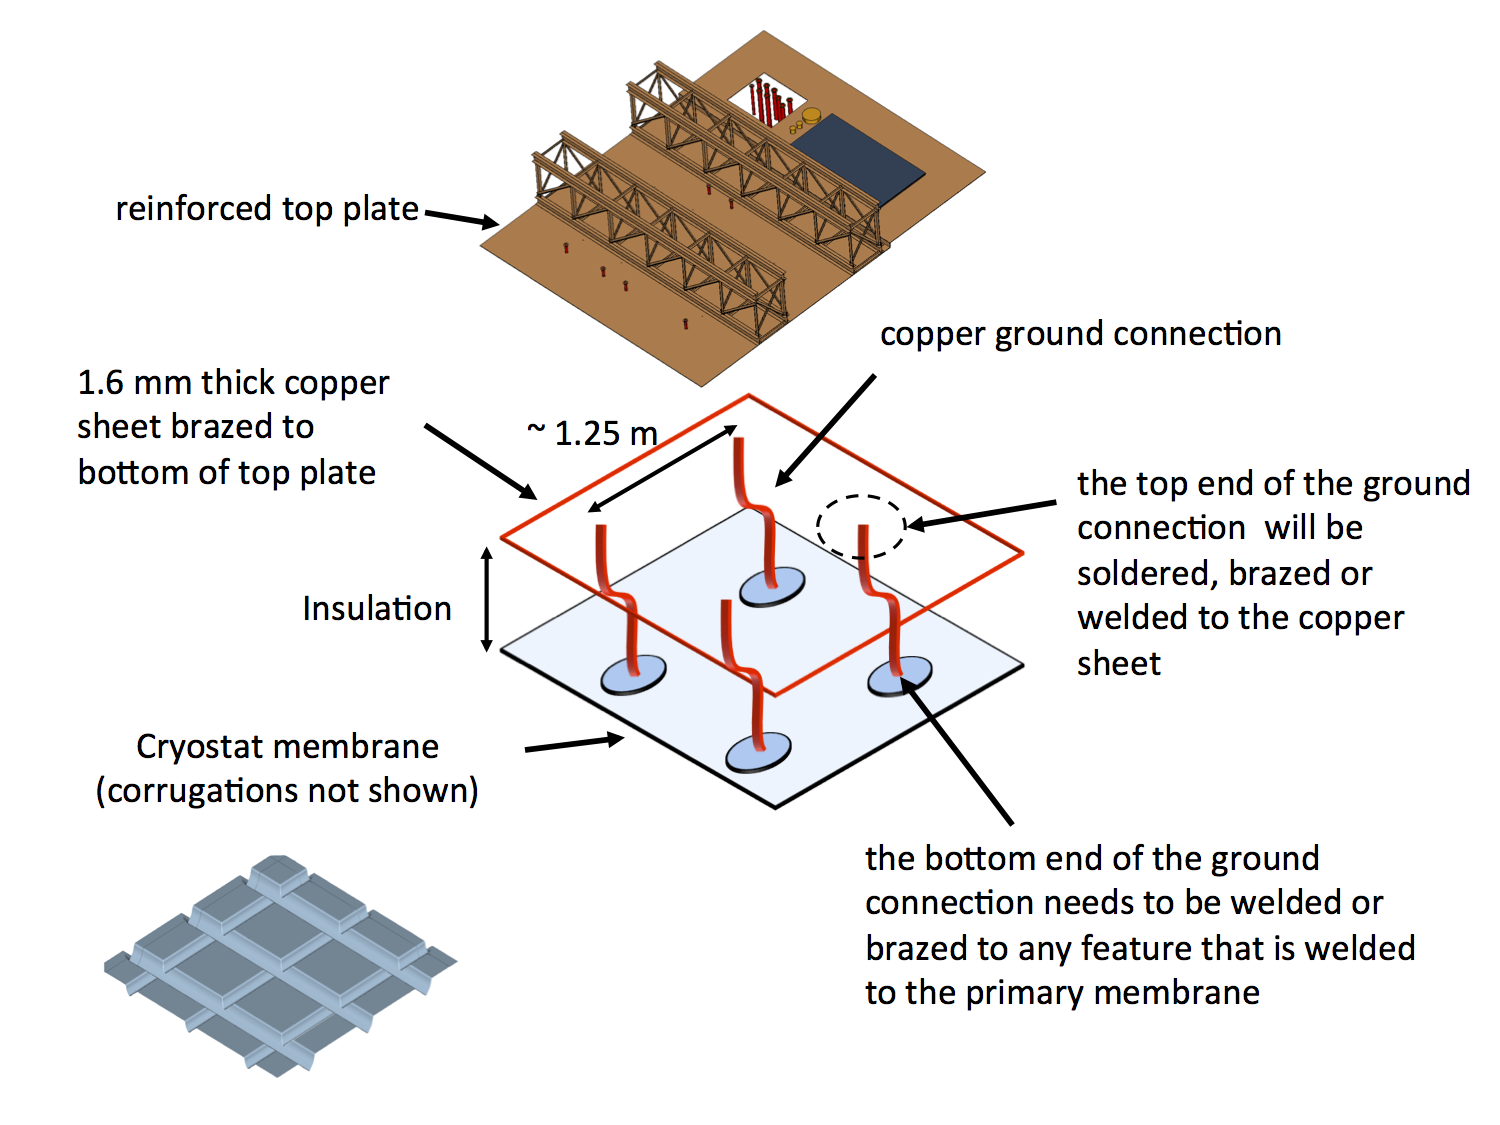
\includegraphics[width=.95\textwidth]{figures/cryostat-top-plate-gnd} 
\caption[Top plate grounding layout]{\label{fig:top-plate-gnd}Top plate grounding layout}
\end{center}
\end{figure}

\textbf{Leak prevention}

The primary membrane will be subjected to several leak tests and weld remediation, as necessary. All 
(100\%) of the welds will be tested by an Ammonia colorimetric leak test (ASTM E1066-95) in which 
welds are painted with a reactive yellow paint before injecting a Nitrogen-Ammonia mixture into the 
insulation space of the tank. Wherever the paint turns purple or blue, a leak is present. The developer is 
removed, the weld fixed and the test is performed another time. Any and all leaks will be repaired. The 
test lasts a minimum of 20 hours and is sensitive enough to detect defects down to 0.003 mm in size 
and to a $10^{-7} std-cm^3/s$ leak rate (equivalent leak rate at standard pressure and temperature, 1 bar and 
273 K). To prevent infiltration of water vapor or oxygen through microscopic membrane leaks (below 
detection level) the insulation spaces will be continuously purged with gaseous argon to provide one 
volume exchange per day. The insulation space will be maintained at 70 mbar, slightly above 
atmospheric pressure. This space will be monitored for changes that might indicate a leak from the 
primary membrane. Pressure control devices and safety relief valves will be installed on the insulation 
space to ensure that the pressure does not exceed the operating pressure inside the tank. The purge gas 
will be recirculated by a blower, purified, and reused as purge gas. The purge system is not safety-
critical; an outage of the purge blower would have negligible impact on LAr purity.

%%%%%%%%%%%%%%%%%
\subsection{Cryostat size from TPC dimensions (Move to begining of sec 4 per DM) }

The minimum internal size of the cryostat is determined from size of the TPC.  At the bottom of the 
cryostat there needs to be a minimum of 0.36 m between the frame of the CPA and closest point on the SS 
membrane.  This is to prevent high voltage discharge between the CPA and the electrically grounded 
membrane. It is foreseen that there would be some cryogenic piping and instrumentation under the TPC.  
There is a height allowance of 0.165 m for this.  There will be access and egress space around the outside 
of the TPC and the membrane walls.  On two sides, 0.15 m of space is reserved for this. The front will have 0.36 mm and the back, where piping and instrumentation for the cryogenic system will be located, 1.20 m.

The support system for the TPC will be located outside the cryostat roof, with a bridge connected to the floor. 
It is the same design solution currently looked at for the DUNE TPC in the LBNF cryostat.  The plan is to model this space similar to what is planned for the far site TPC.  There 
will be 0.82 m of ullage space.  In order to prevent high voltage discharge, the upper most part of the CPA 
needs to be submerged a minimum of 0.5 m below the liquid Argon surface.  The top of the TPC will be 
separated from the membrane by a minimum of 1.1 m.  

Adding all of these to the size of the TPC yields the minimum inner dimensions of the cryostat.  A 
minimally sized cryostat would be 8.8m long, 7.8 m wide and 8.0 m high.  This assumes the TPC will be 
positioned inside the cryostat with the CPAs and end field cages parallel to the walls of the cryostat.  Also 
there is no space allotted for a beam window to enter the cryostat.  Clearance would need to be added if 
it violates any of the current boundaries listed above.  
The current plan is to have the CPAs located in the center of the cryostat with an APA on each side.    

%%%%%%%%%%%%%%%%%
\subsection{Cryogenic System}

Figure~\ref{fig:proposed-LN2-system} outlines the basic scheme of the LN2 supply system, which was 
proposed by CERN for the Short Baseline Program and found to be an appropriate solution for this 
detector as well. The experiment will rely on LN2 tankers for regular deliveries to a local dewar storage, 
which will be sized to provide several days of cooling capacity in the event of a delivery interruption. 
From the dewar storage the LN2 is then transferred to a distribution facility located in the experimental 
hall. It includes a small buffer volume and an LN2 pumping station that transfers the LN2 to the argon 
condenser and other services as needed. The low estimated heat leak of the vessel ($\sim$3.2~kW) and the 
location inside an above ground building allow for use of an open loop system typical of other 
installations operated at Fermilab (LAPD, LBNE 35 ton prototype, MicroBooNE) and at CERN (???). 
Main goal of the LN2 system is to provide cooling power for the argon condenser, the initial cool down of 
the vessel and the detector, and all other services as needed.

 Table~\ref{tbl:cryo-design-parameters} presents the list of 
requirements for the cryogenic system for the Single Phase TPC test at CERN detector.

Figure~\ref{fig:proposed-LAr-system} shows a schematic diagram of the proposed liquid argon system. It is based on the design of the 
LBNE 35 ton prototype, the MicroBooNE detector systems and the current plans for the Long Baseline Far 
Detector.

Main goal of the LAr system is to purge the cryostat prior to the start of the operations (with GAr in open 
and closed loop), cool down the cryostat and fill it with LAr. Then continuously purify the LAr and the boil 
off GAr to maintain the required purity (electron lifetime measured by the detector).

The LAr receiving facility includes a storage dewar and an ambient vaporizer to deliver LAr and GAr to the 
cryostat. The LAr goes through the liquid argon handling and purification system, whereas the Gar 
through the gaseous argon purification before entering the vessel.

The LAr purification system is currently equipped with a filter containing mol sieve and copper beds, and 
a regeneration loop to regenerate the filter itself. Filters containing Oxysorb and Hydrosorb rather than 
mol sieve and copper beds, were also successfully employed. Same concept, but different medium. 
Studies are ongoing to standardize the filtration scheme and select the optimal filter medium for all 
future generation detectors, including this test prototype. 

During operation, an external LAr pump circulates the bulk of the cryogen through the LAr purification 
system. The boil off gas is first recondensed and then is sent to the LAr purification system before re-
entering the vessel.

\begin{table}[htpb]
\caption{Design requirements for the cryogenic system}
\label{tbl:cryo-design-parameters}
\centering
\begin{tabular}{|p{.45\textwidth}|p{.45\textwidth}|}
\hline
 \textbf{ Parameter} & \textbf{Value} \\ \hline
 Location & Preferably not in front of the cryostat (on the beam) \\ \hline
 Cooling Power & TBD based on the heat leak of the cryostat (estimated 3.4~kW), the cryo-piping and all other contributions (cryogenic pumps, etc.) \\ \hline
 Liquid argon purity in cryostat & 10 ms electron lifetime (30 ppt O2 equivalent) \\  \hline
 Gaseous argon piston purge rate of rise & 1.2 m/hr \\ \hline
 Membrane cool-down rate & From manufacturer \\  \hline
 TPCs cool-down rate & \textless40 K/hr,\textless10 K/m (vertically)
 \\ \hline
Mechanical load on TPC & The LAr or the gas pressure shall not apply a mechanical load to the TPC greater than 200 Pascal. \\ \hline
Nominal LAr purification flow rate (filling/ops) & 5.5 day/volume exchange \\ \hline
 Temperature of all surfaces in the ullage during operations & \textless100 K \\  \hline
 Gaseous argon purge within insulation & 1 volume change /day of the open space between insulation panels. \\ \hline
 Lifetime of the cryogenic system & Consistent with the LAr program. TBD. \\ \hline
\end{tabular}
\end{table}

\begin{figure}[htb]
\begin{center}
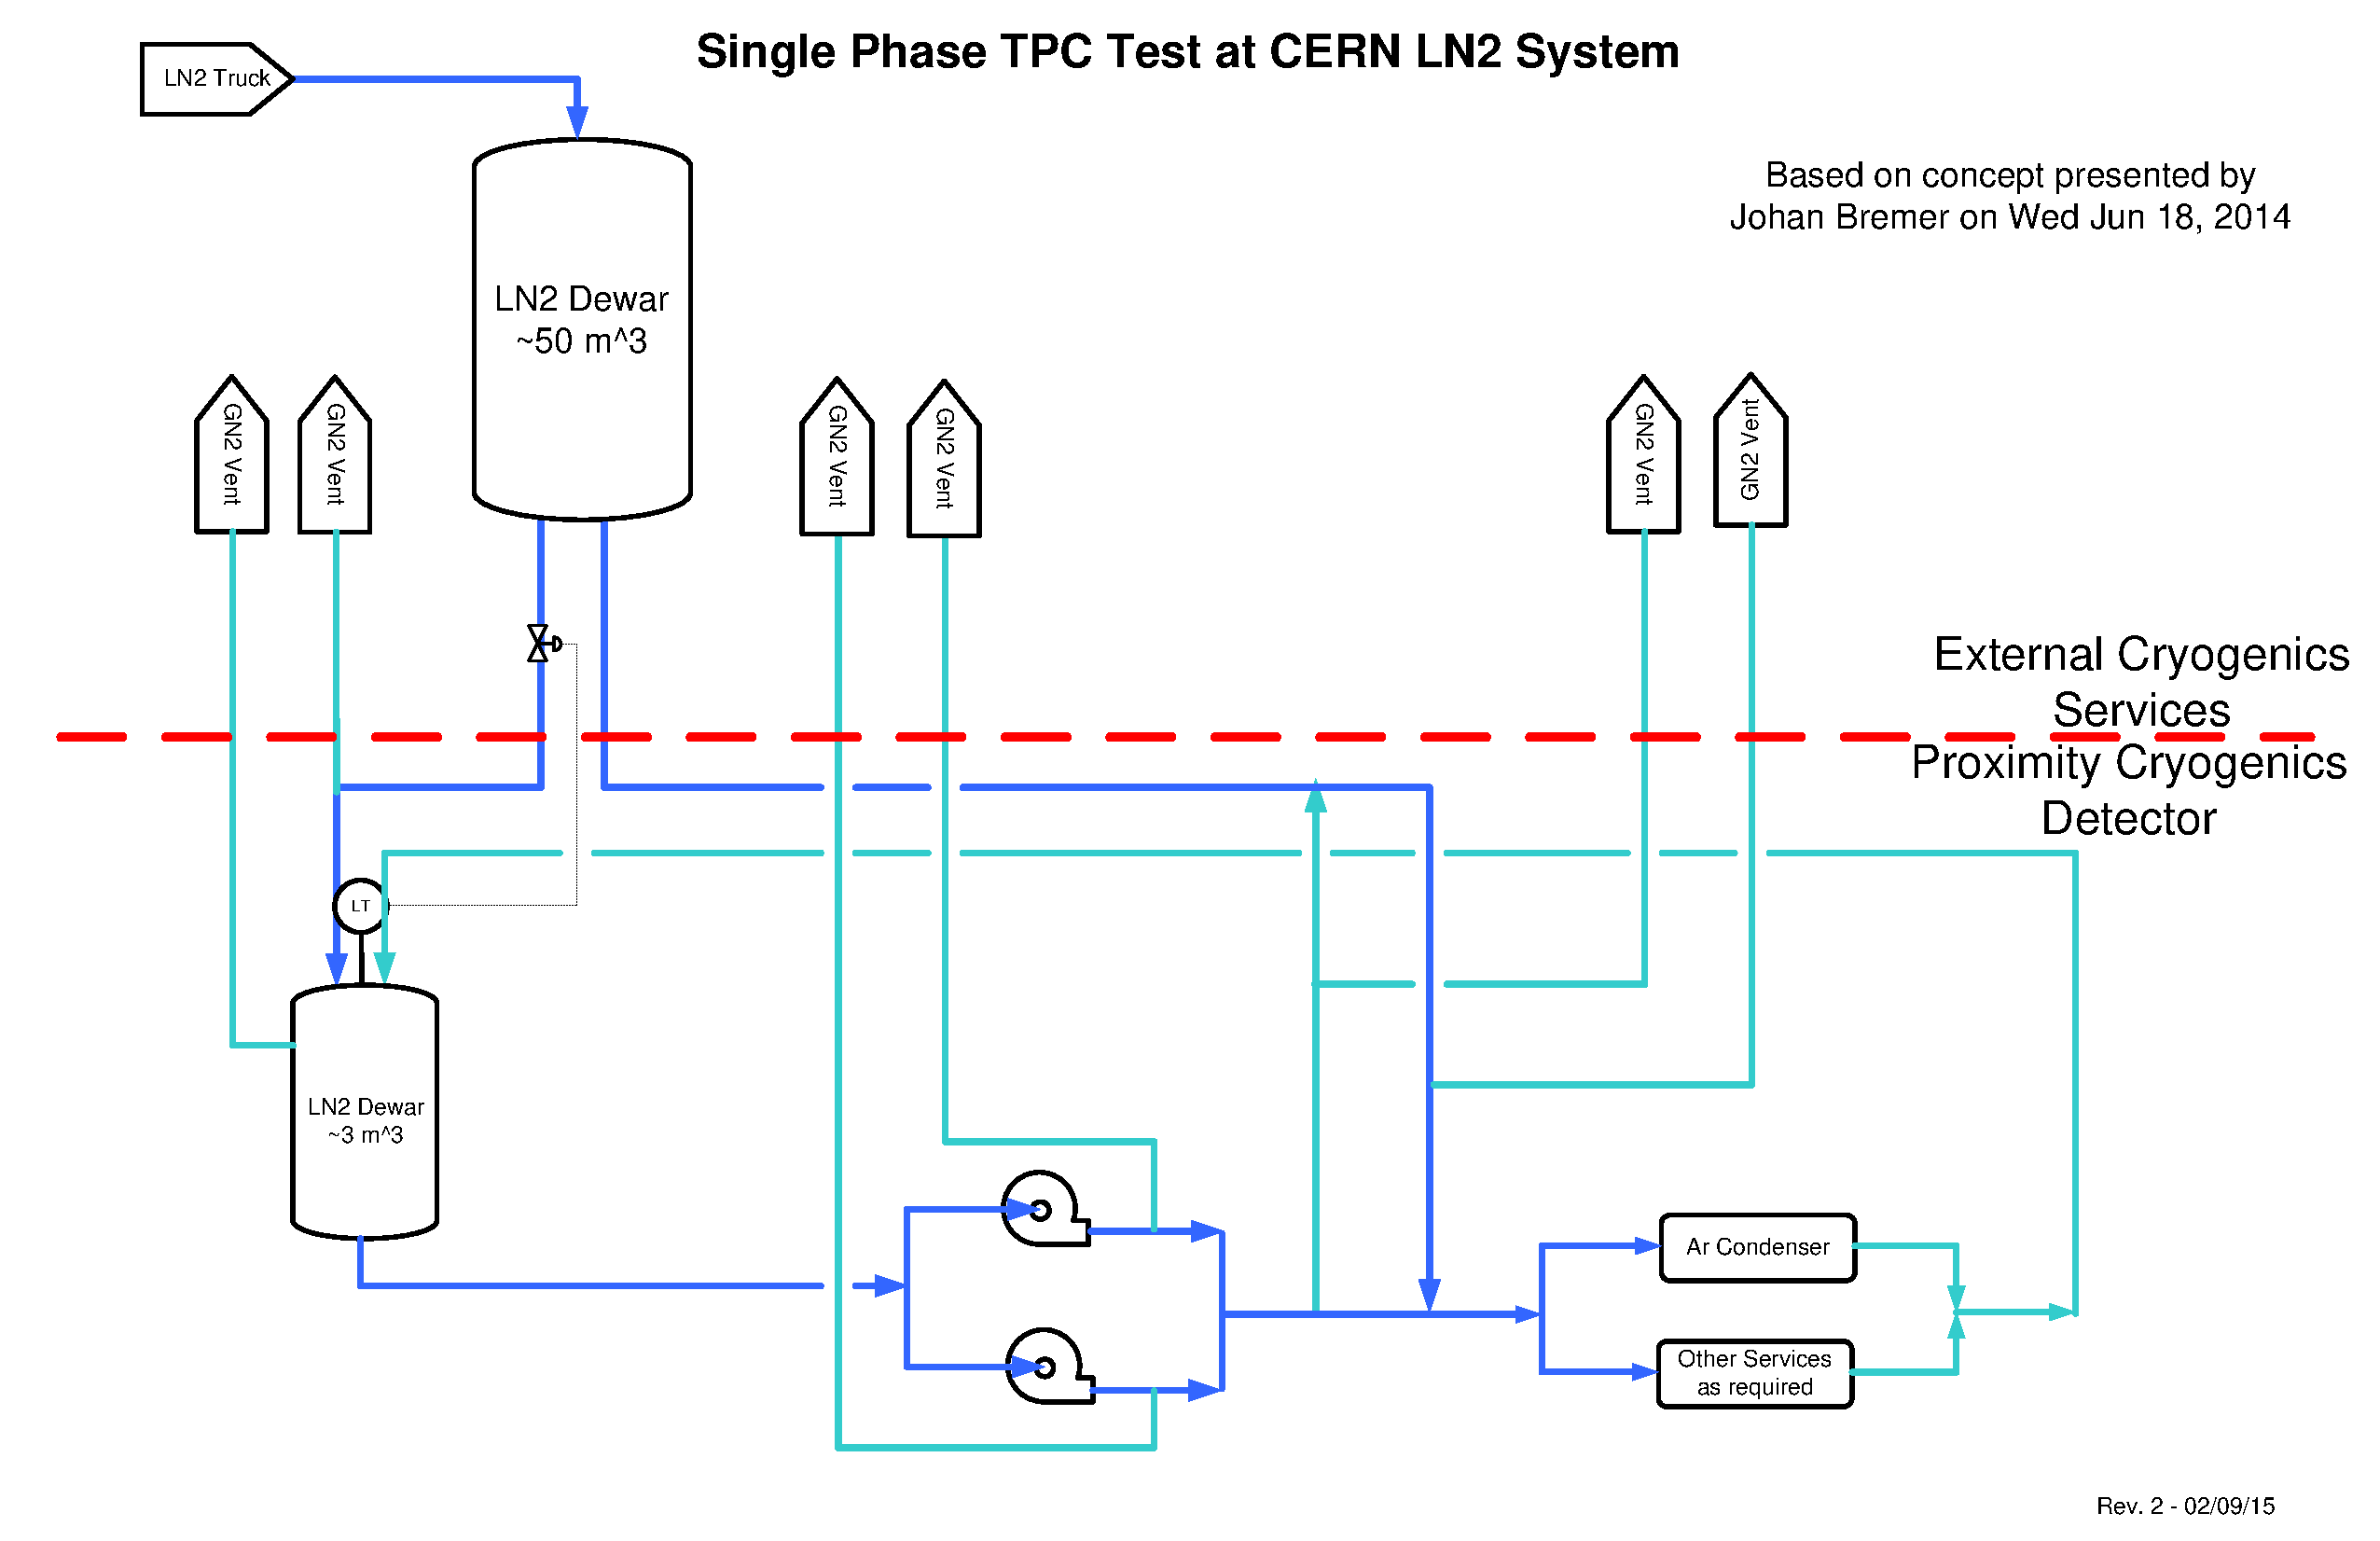
\includegraphics[width=.75\textwidth]{figures/proposed-LN2-system} 
\caption[Schematic diagram for the proposed LN2 system]{\label{fig:proposed-LN2-system}Schematic diagram for the proposed LN2 system}
\end{center}
\end{figure}

\begin{figure}
\begin{center}
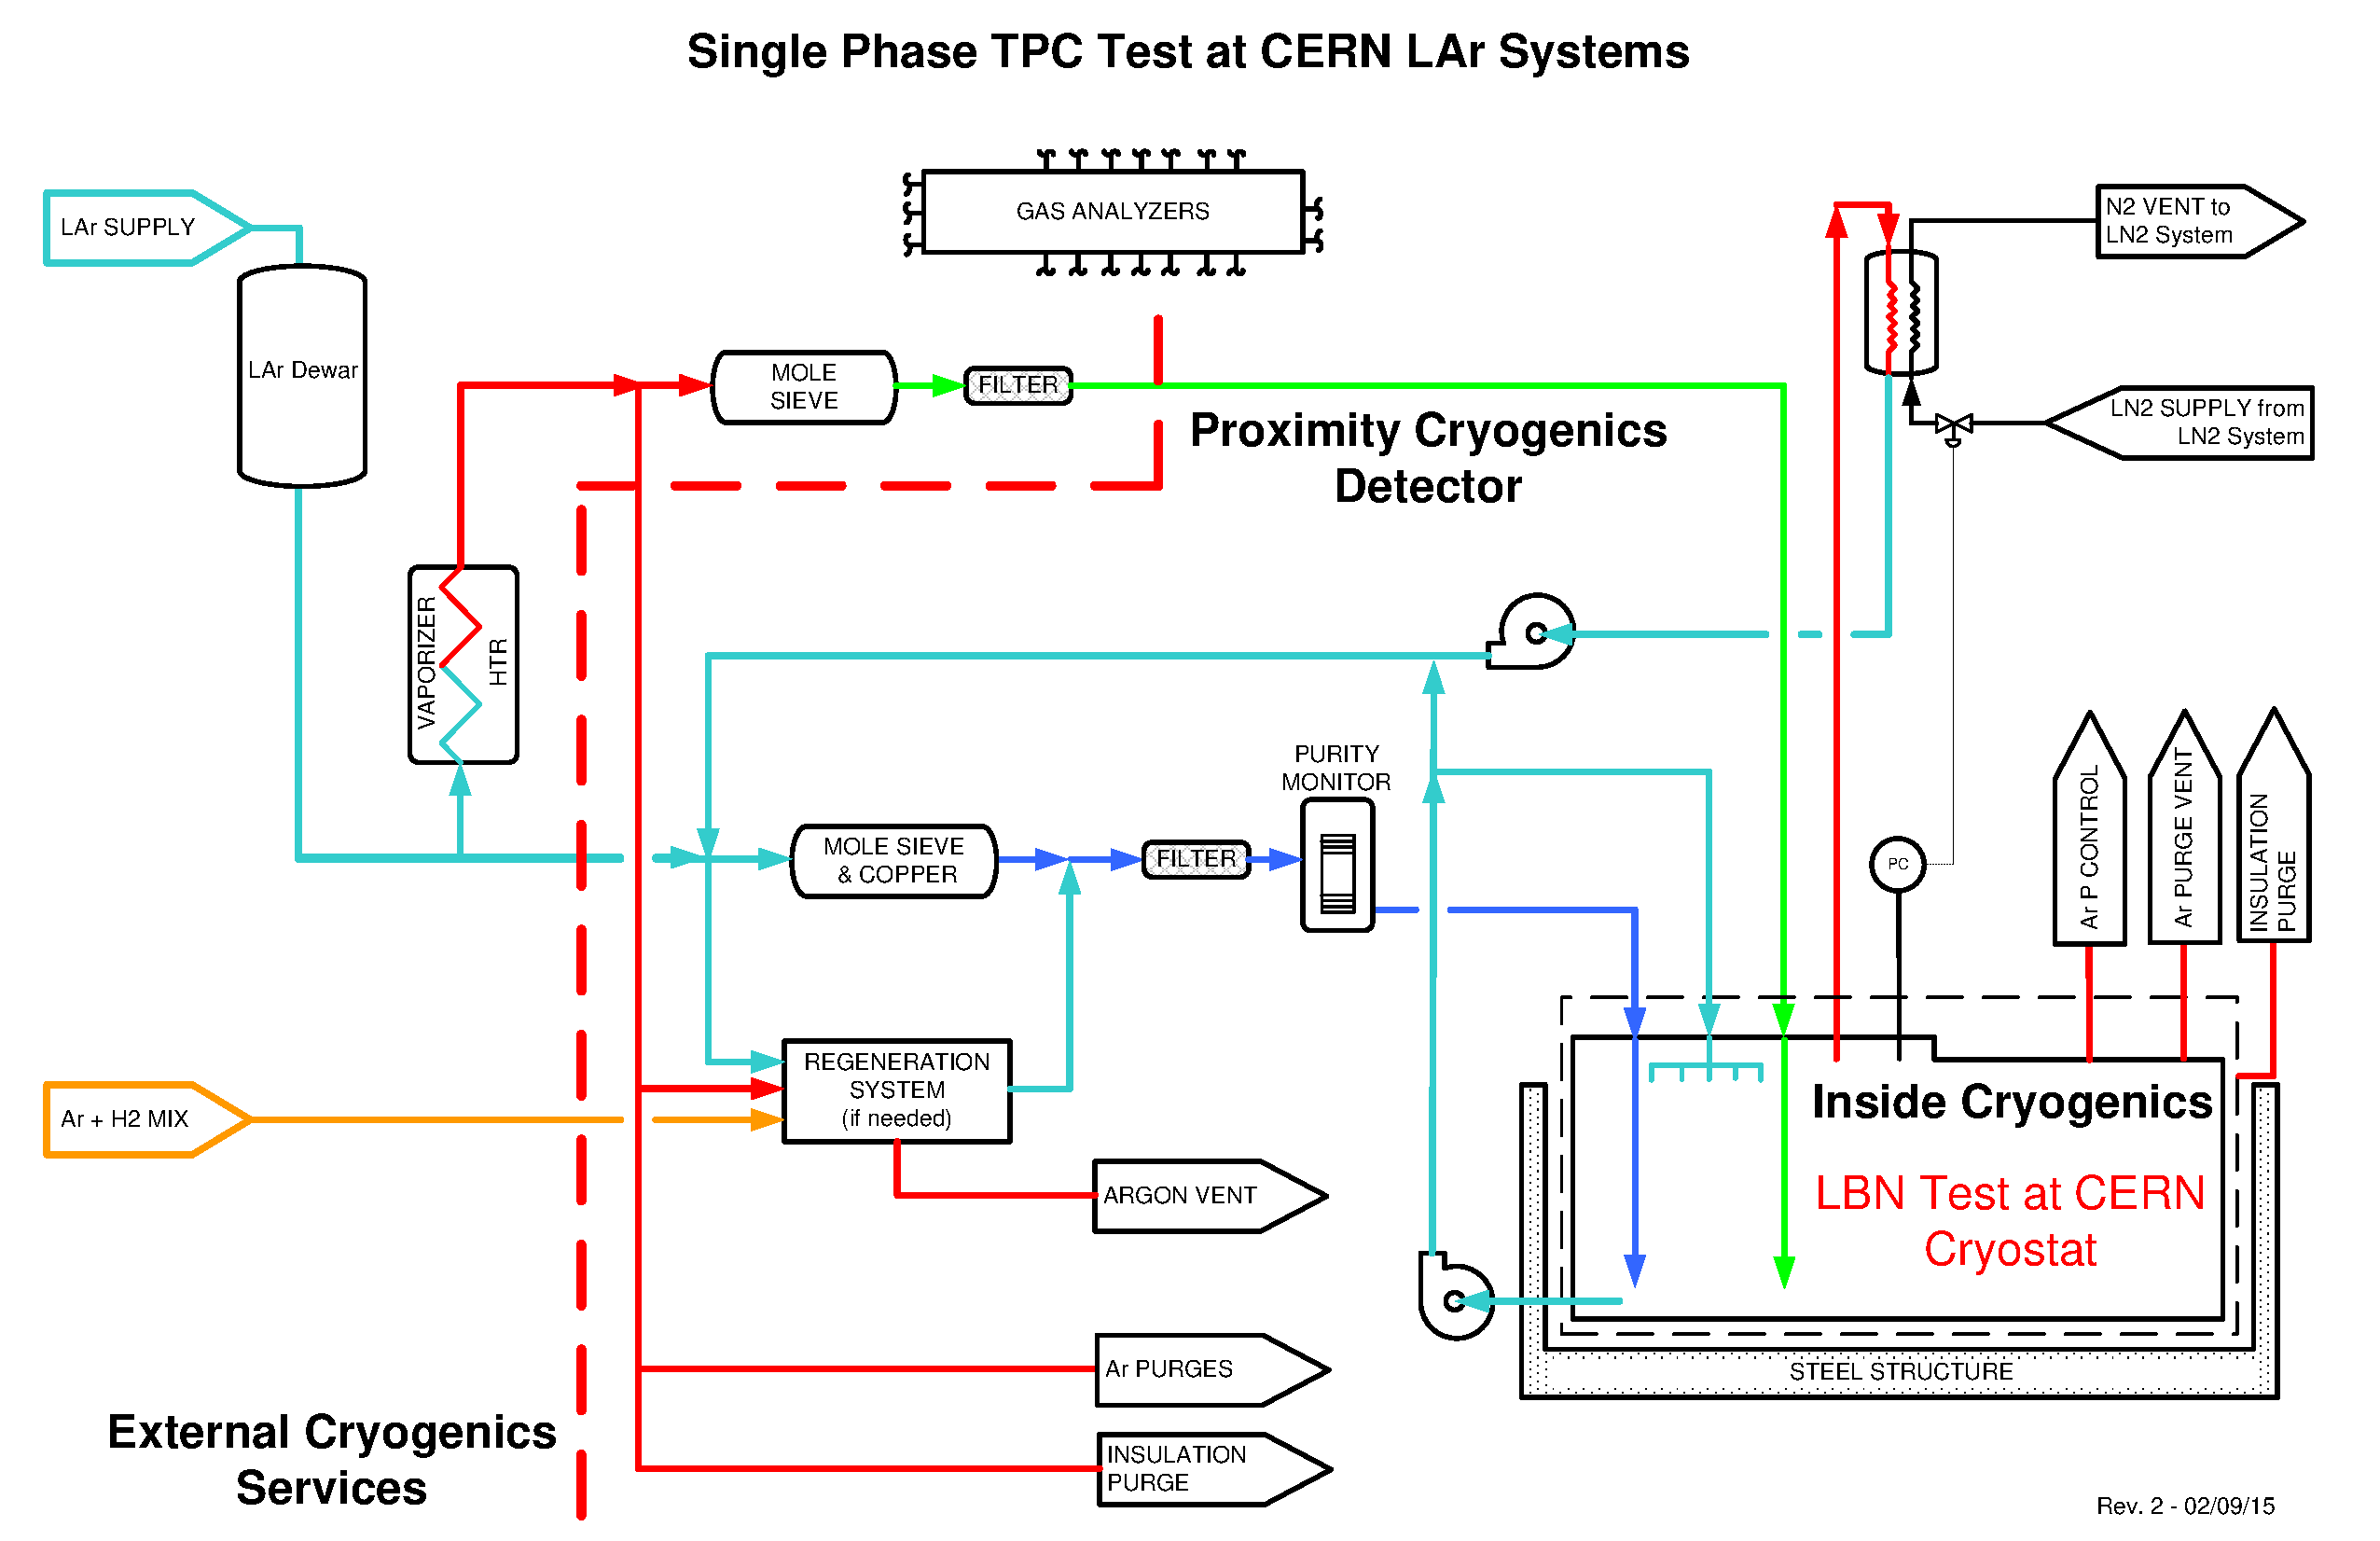
\includegraphics[width=.75\textwidth]{figures/proposed-LAr-system} 
\caption[Schematic diagram for the proposed LAr system]{\label{fig:proposed-LAr-system} Schematic diagram for the proposed LAr system}
\end{center}
\end{figure}



	
\section{Calibration}
	\label{calibration}
%\subsection{Calibration}
The design of the calibration system for DUNE-PT pursues two principal goals. The first is to calibrate the detector itself to
provide high quality data for successive data analysis and the second is to test and optimize the calibration tools themselves for future
use in the DUNE far detectors.

The accuracy of track and kinematics reconstruction and particle identification largely relies on the knowledge of the electric field map, purity map, and temperature inside the active detector volume. The electric field in the drift region, designed to be a uniform 500 V/cm, could vary at different locations due to sagged wires, misalignment and imperfections in the field cage. 


The electric field could also be distorted by the space charge.  Electrons and ions which are generated by the passing of high energy particles drift in opposite directions to anode and cathode planes, respectively. The electrons drift at about 1.6 mm/$\mu s$ and take 2.25 ms to travel the maximum distance between APAs and CPAs. The ions, drifting at $\sim$ 8$\times 10^{-6}$~mm/$\mu s$, can take up to 7.5 minutes to travel the same distance. \\
The surface cosmic ray flux entering the detector imposes a large space-charge effect to the detector. 
%The magnitude of the distortion of the electric field is expected to be on the same order as the microBooNE detector which is also on the surface.  An example of the electric field distortion simulated in the microBooNE detector is shown in Fig.~\ref{fig:space_charge}.
%\begin{figure}[h!]
%  \centering
%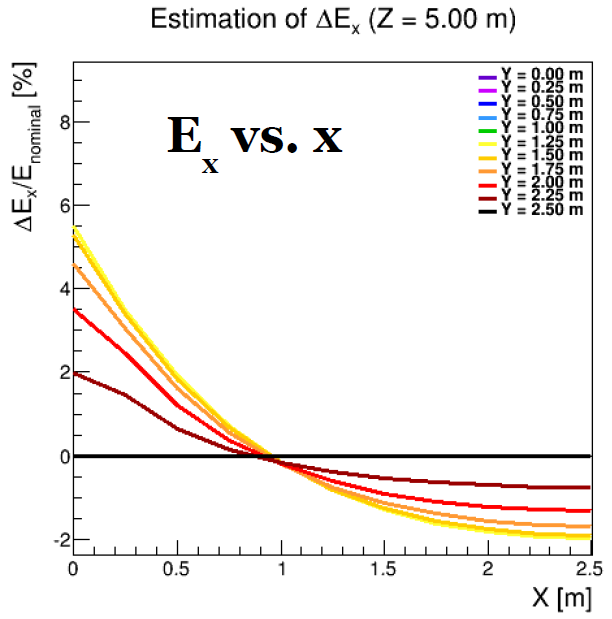
\includegraphics[width=0.49\textwidth,height=6.0cm]{figures/spacechargeEvsx} 
%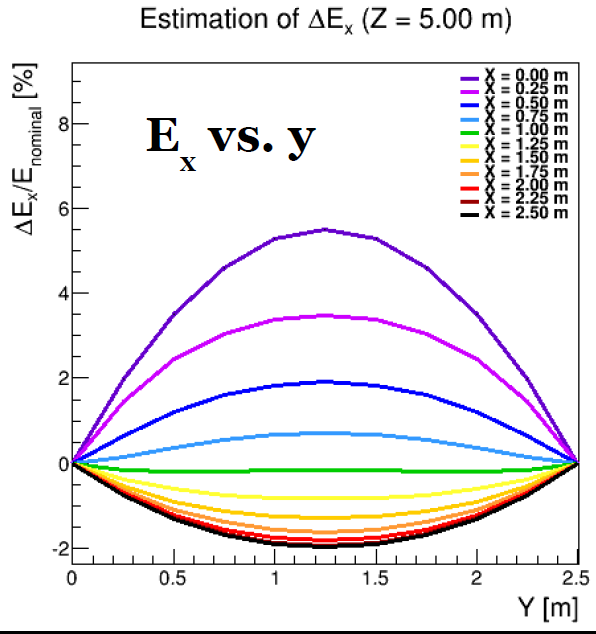
\includegraphics[width=0.49\textwidth,height=6.0cm]{figures/spacechargeEvsy} 
%  \caption{Fractional deviation of the microBooNE drift field $E_{x}$ as a function of position due to space charge effects.  The figure on the left shows the variation as a function of the distance between the cathode (x = 0) and the anode (x = 2.5 m).  The figure on the right shows the variation as a function of the vertical position.  The plots are from \cite{ref:space_charge}.
%{\color{red}  combine e+e-, improve information content (y-axis, change colors, etc )
%}
%}
%\label{fig:space_charge}
%\end{figure}
Distortion of the electric field could result in centimeter levels of uncertainty in position reconstruction and can also make a difference in electron-ion recombination and light output. 

The temperature of liquid argon affects the electron drift velocity and has a gradient of about -1.9\%/K. Precision measurement of temperature could be easily achieved with commercial silicon diode sensors down to tens of milliKelvin. 

Purity of argon directly affects the amount of surviving electrons, which would be used to estimate the amount of energy deposited in that wire space. This energy deposition, dE/dx, is a key quantity for particle identification. Monitoring argon purity is also essential for the operation of the experiment.

Multiple means should be employed to measure the electric field, the purity of liquid argon and its temperature. 
The presently foreseen calibration equipment includes:
\begin{itemize}
\item Gas purity analyzers
\item Liquid purity monitors
\item Temperature sensors
\item Laser calibration system
\item Muon detector system
\end{itemize}

The gas purity analyzers for oxygen and H$_{2}$O are commercially available. These analyzers measure purity down to a few parts per billion (ppb). They are not directly measuring the liquid argon purity in the detector but can be installed outside of the detector and take samples from various points of the cryogenic system and thereby provide an overview of the detector system.

Liquid purity monitors are small size TPCs with light sources that generate electrons via photoelectric effect and electronics to read out the amount of electrons in the cathode plane and anode plane. The electron lifetime can be derived by comparing the number of surviving electrons with those generated. The electron lifetime is a direct estimator of the argon purity.
Multiple liquid purity monitors will be installed at a variety of locations (close to and far from the recirculation inlet) and at different heights.

The temperature of liquid argon varies as a function of the pressure of the detector by a little less than 1~K/psi.  
Silicon diode sensors with accuracy as little as $\sim$ 20 mK will be installed at multiple locations in the detector.

To measure and calibrate electric field, purity, electron lifetime and drift speed in-situ, a laser system and a muon detector are foreseen. 
Both systems, each with particular pros and cons, use ionization-particle paths to measure the above quantities.\\
%
The {\bf laser calibration system} employs a high power ultra-violet (UV) laser to ionize the liquid argon. The 266 nm UV photons have energy of 4.66 eV. Three photons could ionize one argon molecule (ionization potential for liquid argon is 13.78 eV). 
A laser beam is directed into the TPC region via a steerable feedthrough, which allows reflection of the laser beam to various regions of the 
active detector volume. 
The laser energy is about 10 mJ, which corresponds to 10$^{16}$ UV photons, and has sufficient energy to produce 
a straight (long Rayleigh scattering length) and uniform ionization path. Due to the size of the laser beam, about 1 cm in diameter, 
the electrons are generated in a relatively large space, and the electron-ion recombination effect is negligible compared to the cosmic ray 
induced ionization. In the proposed TPC configuration with a CPA in the center and two APAs on the outsides, 
the laser feedthrough will be installed outside of the TPC region and in the same plane as the central CPA.
Therefore the laser beam can be directed to both CPA-APA regions. The field cage is designed with multiple slits to allow the laser 
beam to pass to the inside of the TPC. Position detection systems such as SiPMs will be installed on the other side of the field cage 
to measure the position of the laser beam.

The {\bf cosmic muon detector} system serves as an alternative tool to the laser calibration system. Cosmic rays with energies of a few GeV 
have nearly uniform dE/dx in liquid argon with about 2~MeV/cm and generate about 18,000 electrons/cm. % in the 3 mm wire space. 
Given standard values quoted for the cosmic ray muon flux at sea level, we arrive at a number of roughly 200 incident muons per square meters per second.  Taking into account the dimensions of the TPC, we estimate the area of the top face of its rectangular volume to be just over 50~m$^{2}$, which means that the detector will be subject to $\sim10^{4}$ particles per second.  The full electron drift time in liquid argon for a 3.6~m drift length is 2.25~ms, and each readout window for an event will contain three drift time windows which will include data from drift windows before and after the event.  Based on the cosmic rate and the size of the readout window, there is expected to be on average $\sim$68 track segments on top of the actual beam event.  This estimate takes into account the readout of charge that may still be drifting from the window just prior to the triggered one and the loss of charge that is still drifting after the triggered window ends.    Muon detectors are planned to be installed to preferentially measure cosmic rays passing nearly horizontally through the cryostat.
Additional muon counters on top of the cryostat will allow tagging of highly inclined muons and veto of vertical muons. 
  A disadvantage of using muons as a calibration tool compared to a laser beam is that muons could scatter multiple times in passing 
  through more than 7 meters of liquid argon and will therefore not be perfectly straight anymore.
  


%\newpage
\section{Charged Particle Test Beam Requirements} % [$\sim$10 pages; {\color{red} Cheng-Ju}]}
	\label{testbeamreq}
\subsection{Particle Beam Requirements}
The requested beam parameters are driven by the requirement that the results from the CERN test beam should be directly applicable to the future large underground single-phase LAr detector with minimal extrapolation. The CERN test beam data will be used to evaluate the detector performance, to understand the various physics systematic effects, and to provide ``neutrino-like'' data for event reconstruction studies. To satisfy the requirement, the beam parameters must span a broad range of particle spectrum that are expected in the future neutrino experiment. The particle beam composition should consist of electrons, muons, and hadron beams that are charge-selected. The expected momentum distributions for secondary particles from neutrino interactions are shown in Figure~\ref{fig:particle_momenta}. There is a large spread in the momentum distribution with most particles peaked near 200 MeV/c. To cover the momentum range of interest, the momentum of the test beam should step from 0.2 GeV/c up to 10 GeV/c. 

The maximum electron drift time in the TPC is about 2.2 ms. So, to minimize pile-up in the TPC, the planned beam rate should be around 200 Hz.  Since the single-phase TPC consists of two drift volumes, it is desirable to aim the particle beam so that the hadronic showers are mostly contained in the same drift volume.  The nominal plan is to have the beam enter the cryostat slightly downward at an angle of about 6 degrees. This angle will roughly match the angle at which the neutrino beam enters the liquid argon cryostat at the far detector for the DUNE experiment. Along the horizontal plane, the beam should enter the cryostat with an angle of about 10 degrees to avoid pointing the beam perpendicular to the electron drift in the TPC.  We also plan to take some data with the beam entering a different region of the TPC, and may include some data with particles crossing one drift volume to the next.  The summary of the beam requirements are shown in Table~\ref{table:beamspecs}.
%The two beam entry angles and positions with respect to the LAr cryostat are shown in Figures \ref{fig:BP_SideView} and \ref{fig:BP_TopView}. 

%\begin{figure}[h!]
%  \centering
%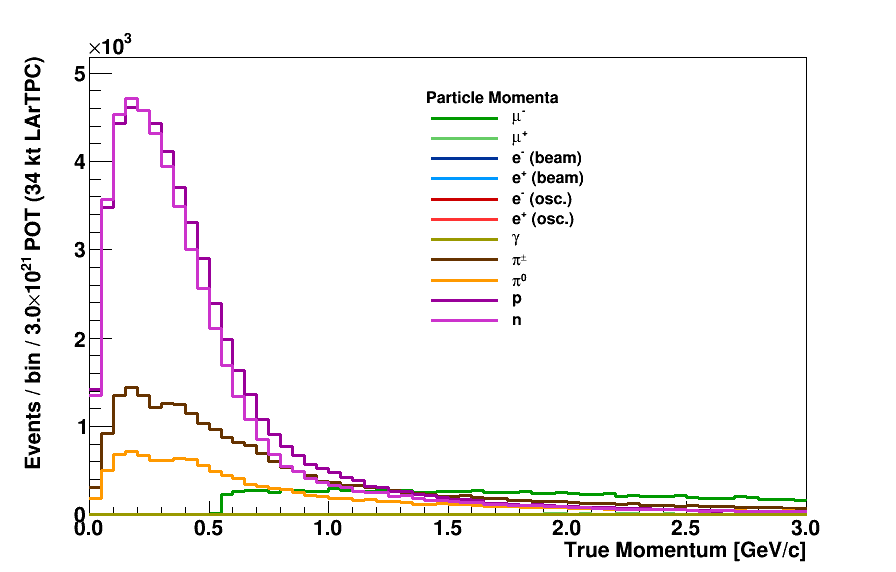
\includegraphics[scale=0.5]{figures/True_Momenta_per_Particle.png}
%  \caption{Particle momenta distributions for particles coming from all fluxes ($\nu_e$, $\nu_\mu$, $\bar \nu_e$ and $\bar \nu_\mu$) at both near and far detector locations.  }
%  \label{fig:particle_momentav2}
%\end{figure}

%\begin{figure}[h]
%  \centering
%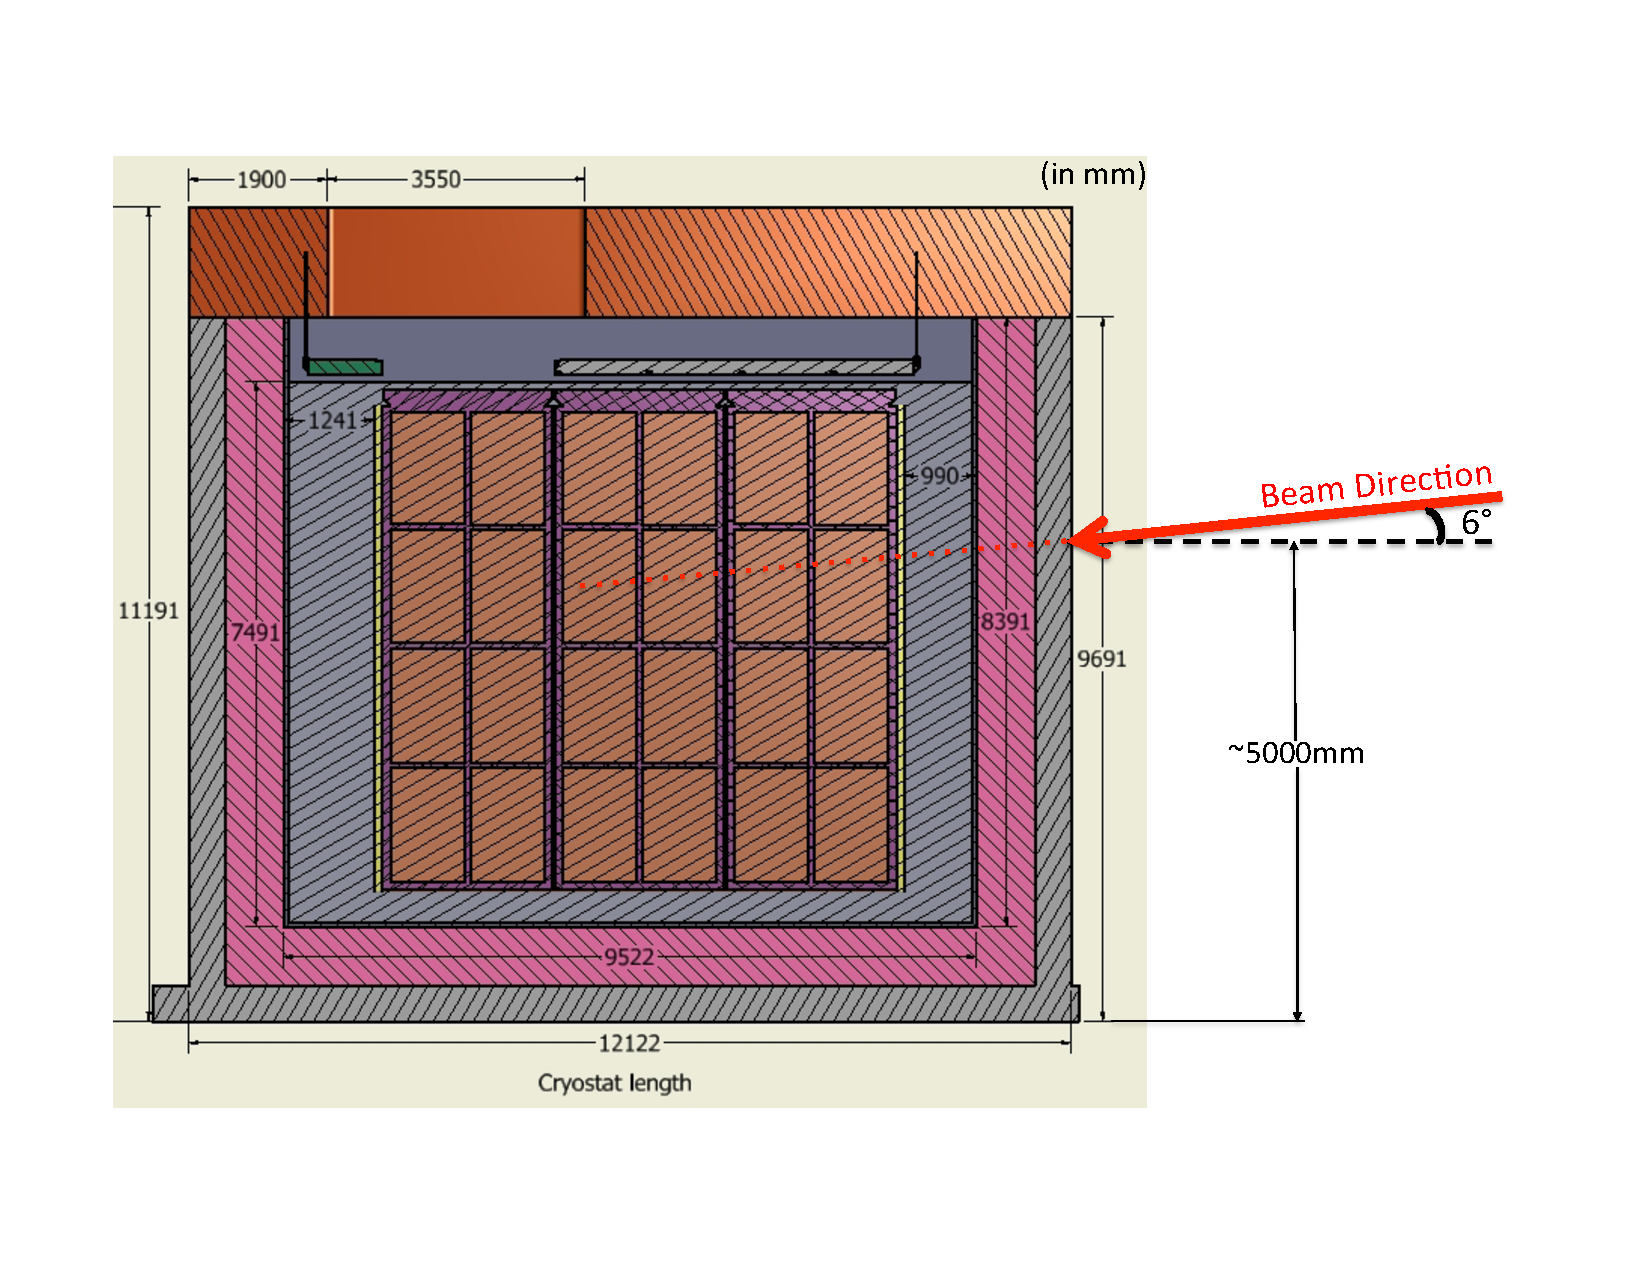
\includegraphics[scale=0.6]{figures/BeamPos_SideView.pdf}
%  \caption{Side view: beam enters the cryostat slightly downward with a dip angle of 6 degrees.  }
%  \label{fig:BP_SideView}
%\end{figure}
%
%\begin{figure}[h]
%  \centering
%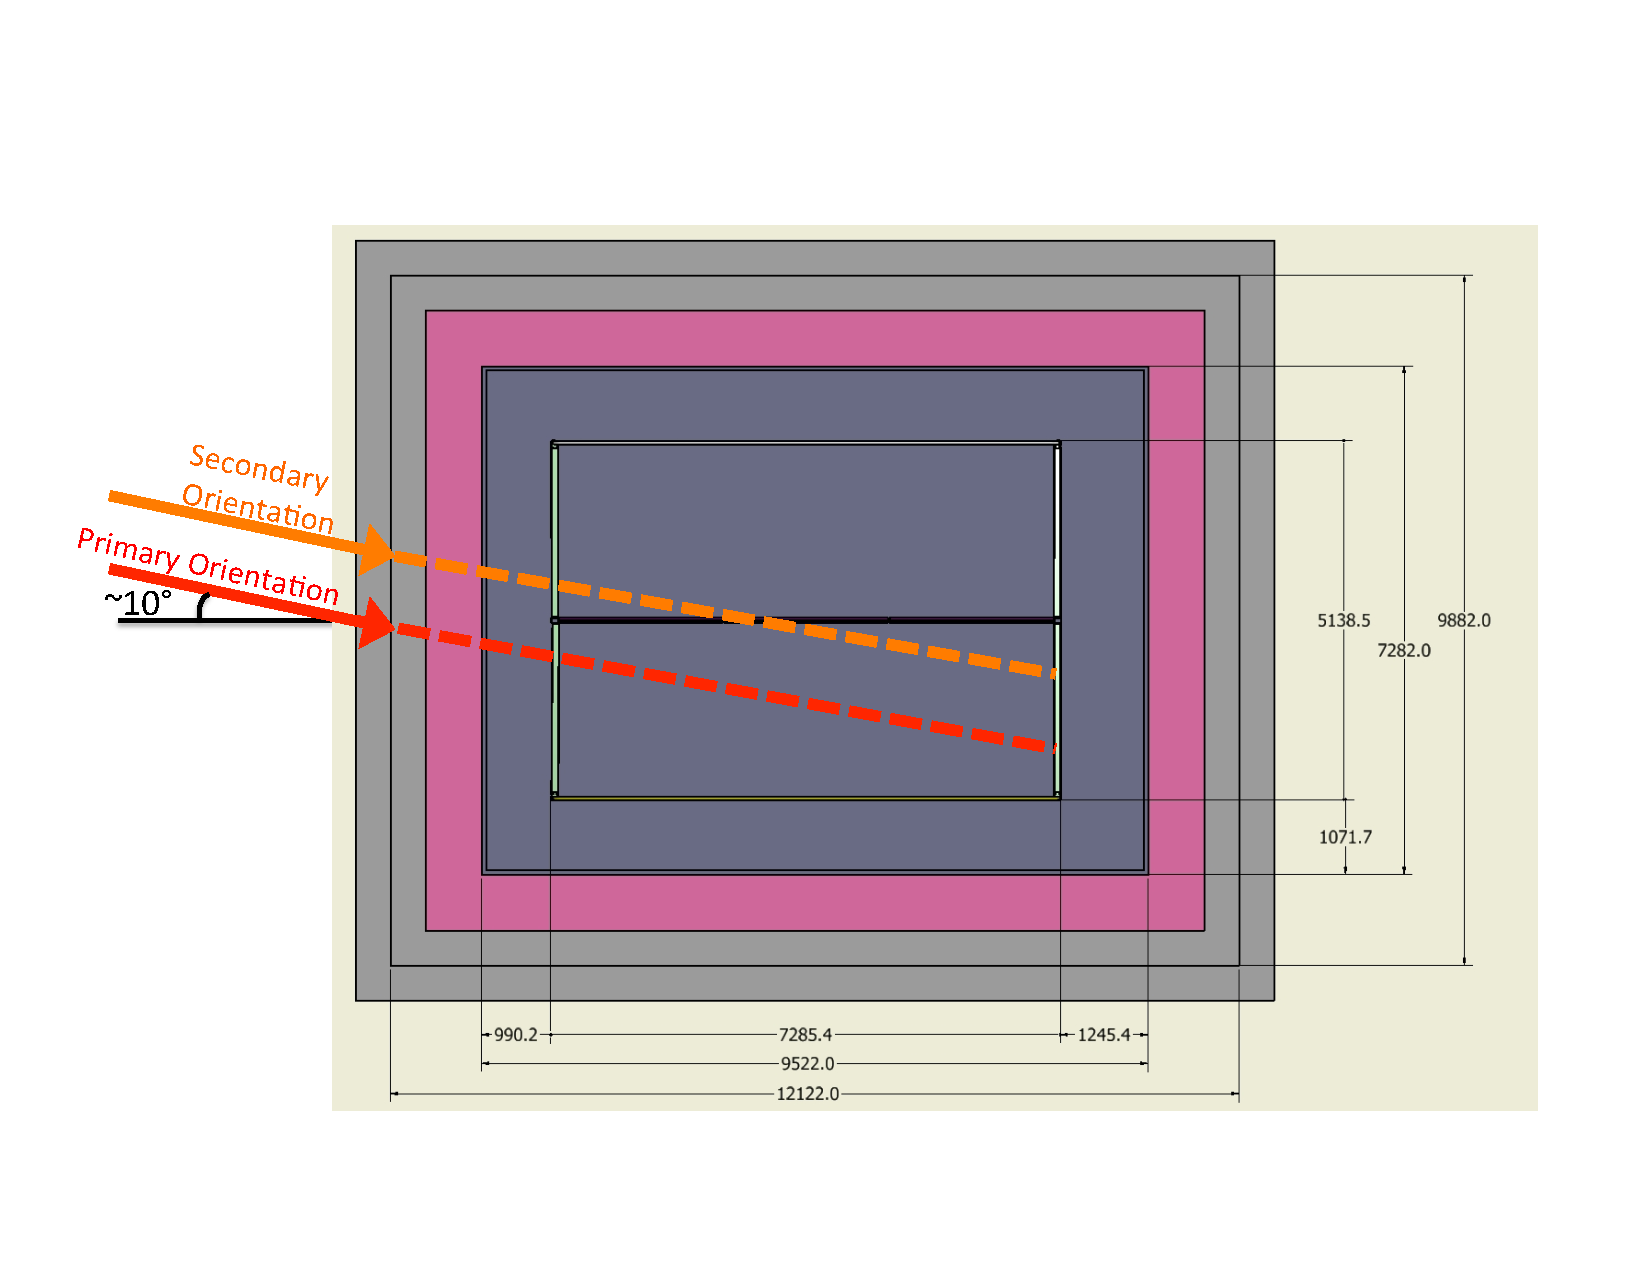
\includegraphics[scale=0.6]{figures/BeamPos_TopView.pdf}
%  \caption{Top view: beam enters the cryostat with an entry angle of about 10 degrees along the horizontal plane. The primary orientation sends the particle beam into one TPC drift volume. The secondary orientation sends the particle beam across the APA. }
%  \label{fig:BP_TopView}
%\end{figure}

\begin{table}[h]
\centering
\begin{tabular}{|c|c|}
\hline
\textbf{Parameter } & \textbf{Requirements}  \\ \hline
  Particle Types        & $e^\pm,\mu^\pm,\pi^\pm$,$K$,$p$  \\ \hline
  Momentum Range   & 0.2 - 10 GeV/$c$ \\ \hline
  Momentum Spread   & $\Delta p/p  < $5 \% \\
  & (limited by the aperture of the magnets)  \\ \hline
  Transverse Beam Size   & RMS(x,y) $\approx$ 10 cm  \\
  & (At the entrance face of the LAr cryostat) \\ \hline
  Beam Divergence & tbd   \\ \hline
  Beam Angle &  $\approx$10$^{\circ}$ \\
  (horizontal plane) &  (w.r.t. the long axis of the cryostat)\\ \hline
  Beam Dip Angle &  $\approx$6$^\circ$ (downward from horizontal)   \\ 
  (vertical plane) &  \\ \hline
  Beam Entrance Position & Multiple beam windows    \\ \hline
  Rates & 200 Hz (maximum)    \\ \hline
\end{tabular}
\caption{Particle beam requirements.}
\label{table:beamspecs}
\end{table}

\subsection{EHN1 H4ext Beamline}
The H4ext is an extension of the existing H4 beamline in Experimental Hall North 1 (EHN1).  To produce particles in the momentum range of interest, a 60-80 GeV/c pion beam from the T2 target is used to generate tertiary beams. The tertiary particles are momentum and charge-selected and transported down H4ext beamline to the experimental area. A conceptual layout of the H4ext beamline is shown in Figure~\ref{fig:H4extPrelim}.  In the Figure, the cryostat for this proposal is located at the lower right hand corner of the plot (in the H4 beam line). The cryostat in the H2 beam line is for the WA105 Collaboration.

\begin{figure}[h]
  \centering
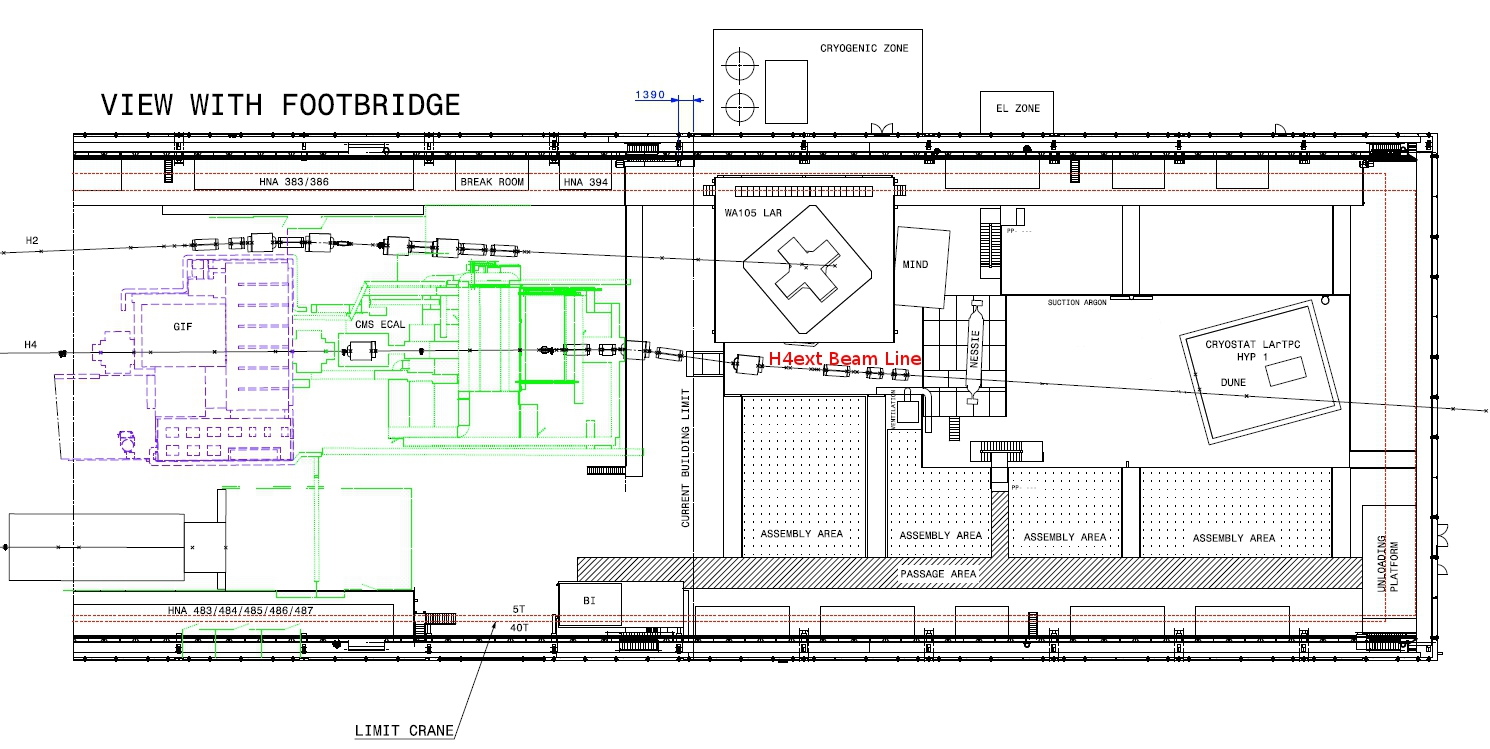
\includegraphics[scale=0.3]{figures/EHN1Ext_Prelim2.jpg}
  \caption{A conceptual layout of the H4ext beamline. The liquid argon cryostat for this proposal is the rotated rectangular box in the lower right hand corner.  }
  \label{fig:H4extPrelim}
\end{figure}

%\subsubsection{Beam Optics}
%[Waiting for inputs from Ilias]

\subsection{Beam Instrumentation}
\label{beaminstrument}
Beam instrumentation provides important information about the characteristics of the beam. It is expected that a series of detectors will be installed along the beam line to measure the particle momentum, identify particle type, and track the particle trajectory.

\subsubsection{Beam Position Detector}
The beam position detector measures the positions of the particle as it traverses the detector. Two detector technologies are under considerations: wire chambers and scintillating fiber trackers. For the nominal setup, one beam position detector is installed upstream and another one downstream of the last bending magnet. This pair provides additional momentum information about the particles as well as the first set of position measurements. Without tracking information, the momentum spread of the beam is expected to be at around 5\% based on the acceptance of the dipole magnets. With additional tracking information, we are likely to be able to measure the momentum of the individual particles to close to one percent level. A third beam position detector is placed right in front of the beam window on the cryostat wall to provide the last position information before the beam enters the cryostat.

\subsubsection{Particle Identification}
In order to have good particle identification over large momentum range, two independent particle identification systems are needed in the beamline. The Time-of-Flight system will be used to cover the lower momentum range while a Threshold Cherenkov detector will be tuned for higher momentum particles. We will require $\geq$ 3$\sigma$ $K$/$\pi$ separation for momentum range from 0.2 to a few GeV/c. Work is in progress to better define the beamline layout to meet the requirements.

\subsubsection{Muon Beam Halo Counters}
The muon beam halo counters is a set of detectors (e.g. plastic scintillator paddles) surrounding the beamline. The main purpose is to tag particles (primarily muons from the upstream production target) that are outside of the beam axis, but may potentially enter the TPC volume. The counter information is used to either veto or simply flag these class of events. The Muon Beam Halo counter can be a subset of the cosmic muon veto system. 

%\subsection{Beam Window on LAr Cryostat}
%This section could be absorbed into the cryostat chapter.


\subsection{Beam Rates and Run Plan}
At the time of this proposal, the beamline design has not been finalized. To estimate the beam rates, we use inputs from a generic target simulation based on 100K 80 GeV $\pi^+$ beam on 15 cm copper target. This $\pi^+$ rate is roughly equivalent to 10\% of a typical SPS spill. The distributions of the tertiary particles from the copper target are shown in Figure~\ref{fig:PionOnCuTarget}. The figure on the left is for postively charged and the figure on the right is for negatively charged tertiary particles. 

\begin{figure}[tbh]
  \centering
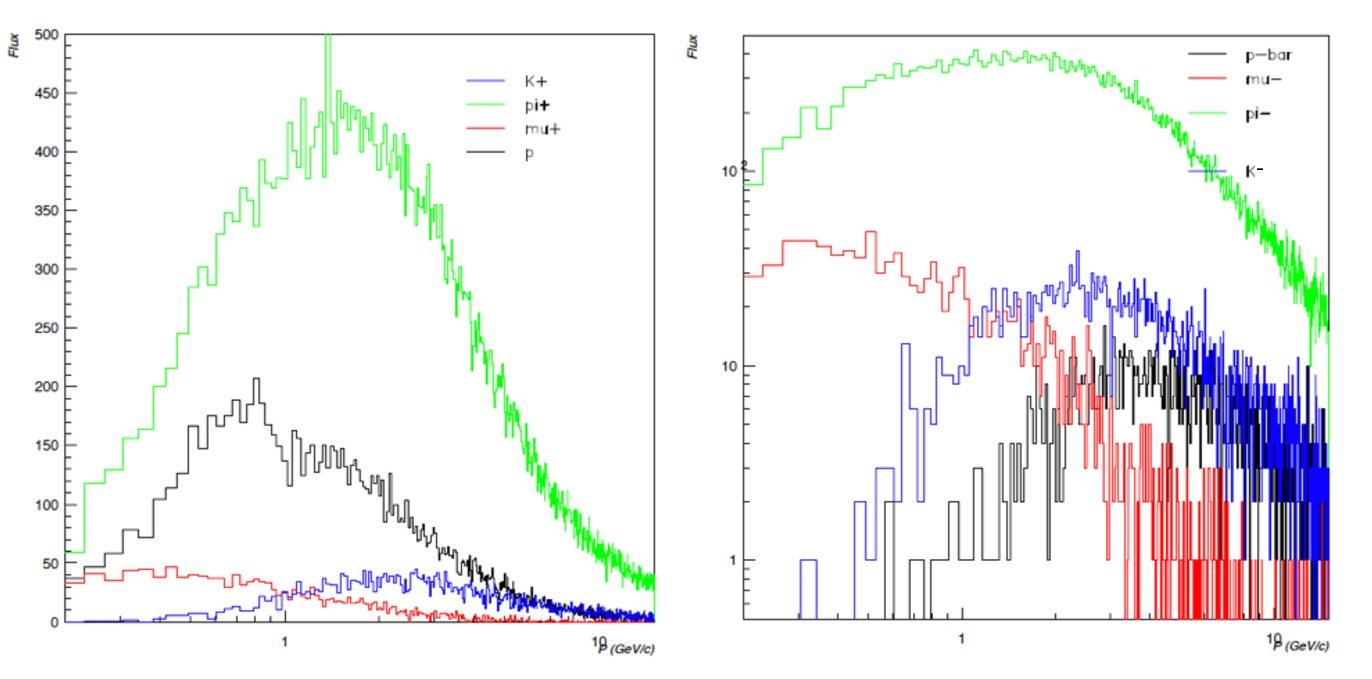
\includegraphics[scale=0.47]{figures/80GeVPion-15cmCuTarget.jpg}
  \caption{Simulation of 100K 80 GeV $\pi^+$ on 15 cm copper target. The figure on the left is for positively charged and the figure on the right is for negatively charged secondary particles from the target. }
\label{fig:PionOnCuTarget}
\end{figure}

To formulate a preliminary beam time request, we assume the hadron beam rates and spectrum as given in Figure~\ref{fig:PionOnCuTarget}. For the beam rate estimates, we account for particle decays assuming the distance from the secondary target to the cryostat to be 30 m. A significant fraction of pions and kaons below 1 GeV/c decay before reaching the liquid argon cryostat. In addition, we also assume the data taking efficiency to be about 50\%. For the electron sample, we expect a different optimized beamline setup to produce a pure electron beam with a flux of about 200 Hz. A preliminary run plan for one configuration is shown in Table~\ref{tab:RunPlan}. The number of spills needed for each momentum bin is driven by the samples highlighted in red or by the requirement that we collect at least 150 spills ($\approx$ 2 hours of beam time) per momentum bin.  This proposed plan satisfies the requested samples as listed in Table~\ref{tab:runsum}, except for kaons less than 1 GeV. Most low momentum kaons produced from the secondary target decay before reaching the liquid argon cryostat. To obtain those samples, we will need to carry out extended runs and trigger exclusively on particles tagged as kaons by either the time-of-flight or the threshold Cherenkov counters.

\begin{table}[tb]
\centering
\rowcolors{0}{gray!30}{gray!30}
\begin{tabular}{|c|c|c|c|c|c|c|}
\hline
\multicolumn{7}{|c|}{\bf Positive Sample} \\ \hline
\bf $P$ & \bf $\#$ of Spills & \bf Time & \bf $\#$ of $\pi^+$ & \bf$\#$ of $\mu^+$ & \bf$\#$ of $K^+$ & \bf$\#$ of p \\ 
\bf (GeV)& & \bf (hours) & & & & \\ \hline
\hiderowcolors
0.2&900 &11&\textcolor{red}{\bf 15K} &180K&$\approx$0&160K\\ 
0.3&200 &3 &\textcolor{red}{\bf 15K} &30K &$\approx$0&50K \\
0.4&150 &\textcolor{red}{\bf 2} &22K &18K &$\approx$0&32K \\ 
0.5&150 &\textcolor{red}{\bf 2} &26K &12K &$\approx$0&38K \\
0.7&150 &\textcolor{red}{\bf 2} &40K &10K &$\approx$0&45K \\
1  &350 &4 &120K&\textcolor{red}{\bf 10K} &$\approx$0&65K \\
2  &600 &8 &320K&\textcolor{red}{\bf 10K} &3K        &130K\\
3  &500 &6 &290K &\textcolor{red}{\bf 5K} &7K        &70K \\
5  &1800&23& 1M &\textcolor{red}{\bf 5K}  &5K        &270K\\
7  &1200&15&660K&\textcolor{red}{\bf 6K}  &3K        &120K\\ \hline
Total &6000&76&2.5M  & 286K  &18K   & 1M\\
\hline \hline
\multicolumn{7}{|c|}{\bf Negative Sample} \\ \hline
\showrowcolors 
\bf $P$ & \bf $\#$ of Spills & \bf Time & 
\multicolumn{2}{|>{\columncolor[gray]{0.83}}c|}{\bf $\#$ of $\pi^-$ }& 
\multicolumn{2}{|>{\columncolor[gray]{0.83}}c|}{\bf$\#$ of $\mu^-$ } \\ 
\bf (GeV)& & \bf (hours) & 
\multicolumn{2}{|>{\columncolor[gray]{0.83}}c|}{}& 
\multicolumn{2}{|>{\columncolor[gray]{0.83}}c|}{} \\ \hline  
\hiderowcolors
0.2&600&8&\multicolumn{2}{|c|}{\textcolor{red}{\bf 15K}} &\multicolumn{2}{|c|}{88K}\\
0.3&200&3&\multicolumn{2}{|c|}{\textcolor{red}{\bf 15K}} &\multicolumn{2}{|c|}{30K}\\
0.4&150&\textcolor{red}{\bf 2}&\multicolumn{2}{|c|}{30K} &\multicolumn{2}{|c|}{18K}\\
0.5&150&\textcolor{red}{\bf 2}&\multicolumn{2}{|c|}{40K} &\multicolumn{2}{|c|}{13K}\\
0.7&150&\textcolor{red}{\bf 2}&\multicolumn{2}{|c|}{50K} &\multicolumn{2}{|c|}{12K}\\
1  &150&\textcolor{red}{\bf 2}&\multicolumn{2}{|c|}{70K} &\multicolumn{2}{|c|}{12K}\\
2  &200&3&\multicolumn{2}{|c|}{135K}&\multicolumn{2}{|c|}{\textcolor{red}{\bf 6K}}\\ \hline
Total  &1600&22&\multicolumn{2}{|c|}{400K}&\multicolumn{2}{|c|}{180}\\ 
\hline 
\hline
\multicolumn{7}{|c|}{\bf Electron Sample} \\ \hline
\showrowcolors 
\multicolumn{3}{|>{\columncolor[gray]{0.83}}c|}{\bf $P$} &\bf $\#$ of Spills&\multicolumn{2}{|>{\columncolor[gray]{0.83}}c|}{\bf Time}&{\bf $\#$ of electron }\\
\multicolumn{3}{|>{\columncolor[gray]{0.83}}c|}{\bf (GeV)} & &\multicolumn{2}{|>{\columncolor[gray]{0.83}}c|}{\bf (hours)}&\\
\hline
\hiderowcolors
\multicolumn{3}{|c|}{0.2,0.3,0.4,0.5,0.7,1,2,3,5,7}  & 150 per bin & \multicolumn{2}{|c|}{2 hours per bin} &{140K per bin} \\ \hline
\multicolumn{3}{|c|}{Total}  & 1500 & \multicolumn{2}{|c|}{20} &{1.4M} \\ \hline
\end{tabular}
\caption{A preliminary run plan for one beam angle and position. The number of spills needed for a given momentum bin is driven by the samples highlighted in red or by the requirement of at least 150 spills per momentum bin.}
\label{tab:RunPlan}
\end{table}

In addition to the above samples with beam at the nominal position, we expect to take some additional data with the beam entering the TPC at different position and angles. Without a detail beamline design, there are still some uncertainties on the actual beam rates. We are working on estimating the amount of beam time required. Based on the current information that we have, the total estimated beam time needed to carry out the physics program (physics samples as listed in Table~\ref{tab:runsum}, multiple angles and beam positions, dedicated kaon runs, etc) in this proposal is in the range of 4 to 6 weeks.
 



\section{Computing, data handling and software} %  [$\sim$3 pages; {\color{red} Maxim/Craig}]}
	\label{computing}
% moved to main doc \section{Computing requirements, data handling and software}

DUNE-PT builds upon the technology and expertise developed in the
process of design and operation of its smaller predecessor, the 35 t detector at Fermilab.
This includes elements of front-end electronics, data acquisition, run controls and related systems. We also expect that for the most part, Monte Carlo studies necessary to support this program will be conducted using software evolved from current (2015) tools. Likewise,
event reconstruction software and analysis tools will rely on the evolving software tools developed for DUNE.

The volume of the recorded data will depend on the number of events to be collected in each measurement,
as specified in the run plan (see Table~\ref{tab:RunPlan}).  Cosmic ray muons have a very large impact on the data volume due to the large detector dimensions and surface operation.

It is optimal to first stage the data collected from DUNE-PT on disk at CERN and then save it to tape also at CERN,
while simultaneously performing replication to data centers in the US. For the latter, Fermilab will be the primary site, with additional data centers at Brookhaven National Laboratory (BNL) and the National Energy Research Scientific Computing Center (NERSC) facility as useful additional locations for better redundancy and more efficient access to the data from a greater number of locations.



%\subsubsection{Cosmic ray muons and readout window}
%\label{readout_windows}
\subsection{Event size estimate and data volume}

The data volume will be dominated by the TPC data. Even though the photon detector as well as other elements of the experimental apparatus (muon counters, trigger systems) contribute to the data stream their contributions to the data volume are expected to be sufficiently small such that realistic data volume estimates can be obtained from the TPC event data sizes alone.

Event sizes can be estimated from "first principles" under the assumption of some event topology and noting the significant amount of cosmic contamination at sea level.  As was shown in Sec.~\ref{calibration}, there is expected to be on average $\sim$68 cosmic muon track segments per readout window and on top of the actual beam event.  Given that a 4 GeV Minimum Ionizing Particle (MIP) will produce on average 80~kbyte of data, the resulting number of particles in a readout window will result in the readout of 6~MB per beam event.  
%This assumes that you have 80~kbyte per 4 GeV mip and that cosmic muons at the surface have an averagae enegy of 4 GeV
%Multiply by (68 muons + 1 beam particle) we get 5.5 MB
In addition to the data associated with the individual particles in the event, channel overhead information needs to be accounted for.   Experience from the 35 t detector at Fermilab indicates that with zero suppression the event overhead amounts to 6~kB per channel for a readout of three drift windows.
%
%This is based on 600kB zero suppressed readout of 3 drift windows in 35 t for 2048 channels.  There are 15,360 channels inn the CERN prototype, corresponding to the proposed TPC which consists of 6 APAs with 2560 channels each. 
%
Since there are 15,360 channels in DUNE-PT, the expected overhead corresponds to 92~MB per event.  The resulting total event size from overhead and charge from individual particles is 100~MB. 
%Background tracks due to cosmic ray particles must be properly identified and accounted for, in order to ensure high quality of the measurements and subsequent detector characterization. Since overlay of cosmic ray muons over beam events is stochastic in nature, the optimal way to achieve this is by recording signals which were produced ``just before'' and ``just after'' the arrival of the test particle from the beam line.  It will be possible because the design of the DAQ contains buffer memory that can be accessed after the trigger decision is made.  This technique will enable us to record and reconstruct either partial or complete background tracks present in the ``main'' event.


%\subsection{Event size estimate and data volume}

%The data volume will be dominated by the TPC data. Even though the photon detector as well as other elements of the experimental apparatus (muon counters, trigger systems) contribute to the data stream their contributions to the data volume are expected to be sufficiently small such that realistic data volume estimates can be obtained from the TPC event data sizes alone.

%Event sizes can be estimated from "first principles" under the assumption of some event topology.  Based on the track range and the number of needed samples to capture the track, a given drift velocity and sample rate a generous over-estimate is that a 1 GeV MIP needs about 20~kbyte and a 5~GeV MIP needs no more than 100~kbyte.  Showering events will require less data for the same energy deposition due to some portion of the activity overlapping in the same voxels.  The estimate assumes that all particles are minimum ionizing so this is another source of over-estimation.  The estimate is based on signals above the threshold of zero-suppression and neglects radioactivity or assumes that signals from radioactivity (predominantly from $^{39}$Ar) are below the zero-suppression threshold.

%This basic estimate serves to set the scale but does neglect channel overhead information that may be useful in interpreting the saved data.  Considering that the beam event readout window will contain $\sim$45 muons with an average energy of 4 GeV, a signal beam event is expected to result in 3.7 MB data record.

%In the LArSoft framework which is presently being used for the 35t detector data are zero suppressed (ZS).  Our assumption is that the nominal readout policy for the bulk of the data will be to use ZS in order to follow the plan for the DUNE FD.  However, even for ZS data LArSoft saves 2 bytes for every channel even if that channel is ZS'ed away. 

%The data event size can be calculated as
%\begin{equation}
%  Event size = (\#channels) \times (clock\, rate) \times (readout \, time) \times (sample \, size)
%\end{equation}
%where the $\# channels$ equals 15,360 channels, corresponding to the proposed TPC which consists of 6 APAs with 2560 channels each, the $clock \, rate$ is 2~MHz, the $readout \, time$ is assumed to be 3 $ \times $ 2.25 ms = 6.75 ms corresponding to three drift times and the $sample \, size$ is 2~bytes.
%
%{\color{red} This results in an event size of $\sim$ 400~Mbyte.\\
%HOW WERE THE 2.5 MB CALCULATED ??! EMAIL FROM BRETT IN RESPONSE TO QIUGUANG AND DATED MAY 5TH INDICATED THAT 2 BYTES PER CHANNEL WERE %ASSUMED ?!\\
%FOR NOW WILL MOVE FORWARD WITH 2.5 MB\\}
%
%
%Based on these assumptions which leave room for optimization
%we arrive at an event size of 2.5 MB/event which is ZS but uncompressed.
%With compression event sizes are expected to reduce to 0.1MB/event (ZS + compressed).
%
%Since each sample is 16 bit (or 12 bit in more recent design), we arrive to the limit of approximately 20MB per single charged track.
%For this class of events, the amount of data will scale roughly linearly with the length of the track, i.e. in cases when a track is
%stopped or leaves the sensitive volume there will be less data. 
%
%Further, in most cases the data will be zero-suppressed by the front-end
%electronics (e.g signals below a certain threshold
%will not be included into the outgoing data stream). 
%The exact data reduction factor will depend on a variety of factors (cf. threshold, which is yet to be chosen), but as a rule of
%thumb it's an order of magnitude. \textit{We conclude therefore the events will typically be a few megabytes in size}. 
%The estimate is supported by Monte Carlo studies.


%In view of the factors due to the cosmic ray muons presented above, the actual beam particle event data will represent only a fraction ofthe total volume being read out.  
%As a concrete example, for an incident
%electron of 4GeV/c momentum MC calculations indicate an average event size of $\sim$2MB, after zero-suppression.
%This is less than 1\% of the estimate quoted above. 

The total particle statistics in the preliminary run plan (Table~\ref{tab:RunPlan}) is approximately 5M events in total.  Taking into account the data load per event, this leads to the estimate of $\sim$500 TB of nominal data volume to be collected in this experiment. 

In summary, we expect that tape storage of $O(1 $PB$)$ size will be required and a somewhat more modest disk space for raw data staging at CERN, for replication purposes.  We envisage storing the primary copy of raw data at CERN, with replicas at additional locations. 
%
Processed and Monte Carlo data placement will require additional resources that are addressed in Section \ref{dataprocess}.


\subsubsection{Data transmission and distribution}
Moving data to remote locations outside of CERN is subject to a number of requirements that include
automation, monitoring and error checking and recovery. 

A number of candidate systems satisfy these requirements and we would like to explore CERN based options and take advantage of 
local know-how. An alternative for which we have expertise and experience is Spade, which was first used in IceCube~\cite{spade_icecube} and then enhanced and successfully utilized in the Daya Bay experiment~\cite{spade_dayabay}.


\subsection{Databases}
Databases will be required to store Run Logs, Slow Control records and detector conditions, as well as (offline) calibration information.

Most database servers will need to be local to the experiment (i.e. at CERN) in order to reduce latency, guarantee reliability and minimize
downtime due to network outages. A replication mechanism is foreseen to make data readily available at the US and other sites.
The volume of data stored in these databases is expected to be modest and of the order of 100~GB.
%Talk to Jon Paley who is in charge of the 35t DB.  He did not have a size for DUNE, but he did have a number for NOvA.  He suggested that the 40kton DUNE will have the same number of channels as NOvA and the NOvA DB uses 200 GB per year.  We should use significantly less.  100 GB is signficantly less than total requested disk space.


\subsection{Computing and software}

%\subsubsection{Distributed Processing}
%\label{distr_proc}

Fermilab provides the bulk of computational power to DUNE via Fermigrid and other facilities. 
We plan to leverage these resources to process the data coming from the DUNE-PT and beam test.

One of the principal goals will be quick validation of the data collected in each measurement, in
order to be able to make adjustments during the run as necessary. 
This is common practice in other experiments which have "express streams" to assess data quality~\cite{atlas_express}.


Given that tracking, reconstruction and other algorithms are in a stage of development with significant improvements
and optimizations expected, the required scale of CPU power needed to process the data are rough estimates.
The estimates we have at this point range from 10 to 100 seconds required by a typical
CPU to reconstruct a single event. 
This means that utilizing a few thousand cores through Grid facilities, it will be possible to ensure timely processing of these data.

To ensure adequate capacity, we envisage a distributed computing model where Grid resources are utilized in addition to Fermilab's computing resources.
As an example, we have had good experience working with the Open Science Grid Consortium.


\subsubsection{Data processing}
\label{dataprocess}

In addition to the raw data preparations being made for offline data handling, processing and storage.
The offline data can be classified as follows:
\begin{itemize}
\item Monte Carlo data, which will contain multiple event samples to cover various event types and other conditions during the measurements with DUNE-PT
\item Data derived from Monte Carlo events, and produced with a variety of tracking and pattern recognition algorithms in order to create a basis for the detector characterization
\item Intermediate calibration files, derived from calibration data
\item Processed experimental data, which will likely exist in several parallel branches corresponding to different reconstruction algorithms being applied, with the purpose of evaluating the performance of the different algorithms.
\end{itemize}

In the latter, there will likely be more than one processing step, thus multiplying data volume. 

The derived data will at most contain a small fraction of the raw data in order to keep the data manageable.
Hence the size of the processed data will likely be significantly smaller than the input (the raw data). 
Given the consideration presented above, we will plan for
$\sim$ $O($1 PB$)$ of tape storage to keep the processed data. 
For efficient processing, disk storage will be necessary
to stage a considerable portion of both raw data (inputs) and one or a few steps in processing (outputs).

Extrapolating from our previous experience running Monte Carlo for the former LBNE Far Detector, we estimate that we will need a few hundred TB of continuously available
disk space. In summary, we expect the need for a few~PB of disk storage at Fermilab to ensure optimal data availability and 
processing efficiency. 

\subsubsection{Data distribution}
We foresee that data analysis (both experimental data and Monte Carlo) will be performed by collaborators residing in many 
institutions and geographically dispersed. In our
estimate above, we mostly outlined storage space requirements for major data centers like CERN and Fermilab. When it comes to making these data available to collaborators, we will utilize a combination of the following:
\begin{itemize}
\item Managed replication of data in bulk, performed with tools like Spade. Copies will be made according to wishes and capabilities of participating institutions.
\item Network-centric federated storage, based on XRootD. This allows for agile, just-in-time delivery of data to worker nodes and workstations over the network. This
technology has been evolving rapidly in the past few years, and solutions have been found to mitigate performance drops due to remote data access, by implementing caching and other techniques.
\end{itemize}

In order to act on the latter item, we plan to implement a global XRootD redirector, which will make it possible to transparently access data from anywhere.
A concrete technical feature of storage at Fermilab is the dCache network which has substantial capacity and can be leveraged
for the needs of the DUNE-PT data analysis. This dCache instance is equipped with a XRootD ``door'' which makes it accessible to the outside world, subject
to proper configuration, authentication and authorization.


Copies for a significant portion of raw and derived data are planed to be hosted at NERSC and also at Brookhaven National Laboratory.
These two institutions have substantial expertise  in the field of data handling and processing at scale and will serve as ``hubs'' for data archival and distribution.


\subsubsection{Software infrastructure}

The DUNE-PT effort will benefit from utilizing simulation toolkits, tracking and other reconstruction
that have and continue to be developed for DUNE, the 35 t detector and the short baseline program at Fermilab as well as the 
neutrino platform development efforts and in particular the WA105 experiment.

The software tools will need to be portable, well maintained and validated. To ensure that this happens,
we plan to establish close cooperation among participating laboratories and other research institutions.



%\end{document}



\section{Installation and infrastructure}  % [5 pages; {\color{red} David/Jack/Cheng-Ju/Thomas}]}
	\label{nuplatform}

%A description of construction of components, facility requirements, layout and constraints follows:

%We propose that the cryostat be housed in the extension of the EHN1 Bat 887 at CERN, where the cryogenic system components will also be located. (moved to sec 7)

%\begin{itemize}

%short description of%location and orientation of cryostat + cryogenics system in EHN1 (David)
%\item {\bf Cryostat construction:}
%The outer steel support structure reduces the time needed for the construction: the structure will be prefabricated in pieces of dimensions appropriate for transportation, shipped to the destination and only assembled in place. Fabrication will take place at the vendor's facility for the most part. This shortens the construction of the outer structure on the detector site, leaving more time for completion of the building infrastructure. If properly designed, a steel structure may allow the cryostat to be moved, should that be desired in the future.

%\item {\bf Cryogenics construction:}
%The outer steel support structure for the cryostat will be prefabricated in pieces of dimensions appropriate for transportation, shipped to the destination and only assembled in place.  Fabrication will take place at the vendor's facility for the most part. This shortens the construction of the outer structure on the detector site, leaving more time for completion of the building infrastructure. If properly designed, a steel structure may allow the cryostat to be moved, should that be desired in the future.

%\item {\bf Detector component construction:} 
%TPC and PDS detector components will be manufactured and submitted to quality assurance procedures at one or more of the potential DUNE detector component production sites. Successively, components will be shipped to CERN for further testing and final assembly into the cryostat. This approach will begin the preparations for the various production sites for the first 10~kt module of the DUNE far detector.

%\item {\bf PDS schedule items:}
%Once the technology has been chosen the PD group will focus on optimizing the selected design with the goal of procurement and assembly taking place in late FY 2016 and early FY 2016. The photon detector paddles will then be tested and shipped to CERN in early FY 2017 for installation into the APAs in late FY 2017 in preparation for installation into the test cryostat and operation in 2018. 

%\item Requirements for staging space, control room, electronics racks, clean room, scaffolding, etc. (Jack)

%\item power requirements and cooling 

%\item ...

%\end{itemize}

%\subsection{Installation}

The interior of the cryostat will be prepared prior to the installation of the TPC.  A series of I-beam support rails will be suspended below the top surface of the cryostat membrane by a series of hangers.  These hangers will be structurally supported by an independent structure above the cryostat.  Decoupling the TPC support from the cryostat structure eliminates the movement of the TPC with the flexure of the cryostat structure from the filling and internal pressure changes of the Argon inside.  The hangers will pass through the top of the cryostat to the independent structure inside a bellows type feedthrough.  These feedthroughs need to be designed to minimize the heat flow into the cryogenic volume.  For the CPAs, the support rails and hangers need to be electrically isolated due to high voltage concerns.  To preserve the ability to reverse the order of the TPC components, all of the support points will be designed to the maximum set of requirements regarding loads and clearances.  

There will be a series of feedthrough flanges located along each of the support rails.  These will be cryogenic flanges where the services for the TPC components can pass through the top of the cryostat.  It is foreseen that each CPA row will require one feedthrough for the high voltage probe to bring in the drift voltage.  The drift voltage is 500 V/cm.  For a drift distance of 3.6~m and 2.5~m, the probe voltages will be 180~kV and 125~kV respectively.  There will be one service feedthrough for each of the APAs.  These feedthroughs will include high speed data connections, bias voltages for the wire planes, control and power for the cold electronics.  

The main TPC components will be installed through large hatches in the top of the cryostat.  This is 
similar to the installation method intended for the detector at the DUNE far site.  These hatches will have an 
aperture approximately 2.0 m wide and 3.5 m long.  Each APA and CPA panel will be carefully tested after transport into the clean area and before installation into the cryostat. Immediately after a panel is installed it will be rechecked. The serial installation of the APAs along the rails means that removing and replacing one of the early panels in the row after others are installed would be very costly in effort and time. Therefore, to minimize the risk of damage, as much work around already installed panels as possible will be completed before proceeding with further panels.
The installation sequence is planned to proceed as follows:

\begin{enumerate}
\item Install the monorail or crane in the staging area outside the cryostat, near the equipment hatch.
\item Install the relay racks on the top of the cryostat and load with the DAQ and power supply crates.
\item Dress cables from the DAQ on the top of the cryostat to remote racks.
\item Construct the clean-room enclosure outside the cryostat hatch.
\item Install the raised-panel floor inside the cryostat. 
\item Insert and assemble the stair tower and scaffolding in the cryostat.
\item Install the staging platform at the hatch entrance into the cryostat.
\item Install protection on (or remove) existing cryogenics instrumentation in the cryostat.
\item Install the cryostat feedthroughs and dress cables inside the cryostat along the support beams.
\item Install TPC panels:
   \begin{enumerate}
   \item Install the CPA panels supported from the center support rail.  These will be installed from the floor of the cryostat.  Access to the top edge will be required by scaffolding.  
   \item Install and connect HV probe for the CPAs.
   \item Perform electrical tests on the connectivity of the probe to the CPAs.
   \item Install first end wall of vertical field cage at the non-access end of the cryostat.  These will be installed from the floor of the cryostat.  Scaffolding will be needed to install the supporting structure and then attach the panels to the structure.  
   \item Test the inner connections of the field cage panels.
   \item Install the first APA and connect to the far end field cage support.
   \item Connect power and signal cables.  This will require scaffolding to access the top edge of the APA.
   \item Test each APA wire for expected electronics noise. Spot-check electronics noise while cryogenics equipment is operating.
   \item Install the upper field cage panels for the first APA between the APA and CPAs  This will require scaffolding to access the upper edge of the APA, CPA and field cage structure.
   \item Perform electrical tests on upper field cage panels.
   \item Repeat steps (f) through (j) for the next five APAs.
   \item Install the lower field cage panels between the APAs and CPAs.  Start at the far end away from the access hatch and work towards the hatch. 
   \item Perform electrical test on lower field cage panels and the entire loop around the TPC.
   \item Remove temporary floor sections as the TPC installation progresses.
   \item Install sections of argon-distribution piping as the TPC installation progresses.
   \item Install the final end wall of vertical field cage at the access end of the cryostat.  These will be installed from the floor of the cryostat.  Scaffolding will be needed to install the supporting structure and then attach the panels to the structure.
   \end{enumerate}
\item Remove movable scaffold and stair towers.
\item Temporarily seal the cryostat and test all channels for expected electronics noise.
\item Seal the access hatch.
\item Perform final test of all channels for expected electronics noise.
\end{enumerate}
 
In general, APA panels will be installed in order starting with the panel furthest from the hatch side of the cryostat and progressing back towards the hatch. The upper field cage will be installed in stages as the installation of APAs and CPA progresses.  After the APAs are attached to the support rods the electrical connections will be made to electrical cables that were already dressed to the support beams and electrical testing will begin. Periodic electrical testing will continue to assure that nothing gets  damaged during the additional work around the installed APAs.  

The TPC installation will be performed in three stages, each in a separate location. First, in the clean room vestibule, a crew will move the APA and CPA panels from storage racks, rotate to the vertical position and move them into the cryostat. Secondly, in the panel-staging area immediately below the equipment hatch of the cryostat, 
% CHECK THIS! I TRIED TO INTERPRET RUSS'S COMMENTS. -- ANNE
a second crew will transfer the panels from the crane to the staging platform, where the crew inside the cryostat will connect the panels to the rails within the cryostat. A third crew will reposition the movable scaffolding and use the scaffold to make the mechanical and electrical connections at the top for each APA and CPA as they are moved into position.  

The requirements for alignment and survey of the TPC are under development. Since there are many cosmic rays in the surface detector and beam events, significant corrections can be made for any misalignment of the TPC. The current plan includes using a laser guide or optical transit and the adjustment features of the support rods for the TPC to align the top edges of the APAs in the TPC to be straight, level and parallel within a few millimeters. The alignment of the TPC in other dimensions will depend on the internal connecting features of the TPC.  The timing of the survey will depend on understanding when during the installation process the hanging TPC elements are in a dimensionally stable state. The required accuracy of the survey is not expected to be more precise than a few millimeters.  






\subsection{Installation}

The outer steel support structure for the cryostat will be prefabricated in pieces of dimensions appropriate for transportation, shipped to the destination and only assembled in place.  Fabrication will take place at the vendor's facility for the most part. This shortens the construction of the outer structure on the detector site, leaving more time for completion of the building infrastructure. If properly designed, a steel structure may allow the cryostat to be moved, should that be desired in the future.

The TPC and PDS detector components will be manufactured and submitted to quality assurance procedures at one or more of the potential DUNE detector component production sites. Successively, components will be shipped to CERN for further testing and final assembly into the cryostat. This approach will begin the preparations for the various production sites for the first 10~kt module of the DUNE far detector.

The interior of the cryostat will be prepared prior to the installation of the TPC.  Several I-beam support rails will be suspended below the top surface of the cryostat membrane by a series of hangers.  These hangers will be supported by an independent structure above the cryostat.  Decoupling the TPC support from the cryostat structure eliminates the movement of the TPC with the flexure of the cryostat structure from the filling and internal pressure changes of the Argon inside.  The hangers will pass through the top of the cryostat to the independent structure inside a bellows type feedthrough.  These feedthroughs need to be designed to minimize the heat flow into the cryogenic volume.  For the CPAs, the support rails and hangers need to be electrically isolated due to high voltage concerns.  To preserve the ability to reverse the order of the TPC components, all of the support points will be designed to the maximum set of requirements regarding loads and clearances.  

There will be a series of feedthrough flanges located along each of the support rails.  These will be cryogenic flanges where the services for the TPC components can pass through the top of the cryostat.  It is foreseen that the CPA row will require one feedthrough for the high voltage probe to bring in the drift voltage.  The drift field is 500 V/cm.  For a drift distance of 3.6~m and 2.5~m, the probe voltages will be 180~kV and 125~kV, respectively.  There will be one service feedthrough for each of the APAs.  These feedthroughs will include high speed data connections, bias voltages for the wire planes, control and power for the cold electronics.  

The main TPC components will be installed through large hatches in the top of the cryostat.  This is 
similar to the installation method intended for the detector at the DUNE far site.  These hatches will have an 
aperture approximately 2.0 m wide and 3.5 m long.  Each APA and CPA panel will be carefully tested after transport into the clean area and before installation into the cryostat. Immediately after a panel is installed it will be rechecked. The serial installation of the APAs along the rails means that removing and replacing one of the early panels in the row after others are installed would be very costly in effort and time. Therefore, to minimize the risk of damage, as much work around already installed panels as possible will be completed before proceeding with further panels.
 
In general, APA panels will be installed in order starting with the panel furthest from the hatch side of the cryostat and progressing back towards the hatch. The upper field cage will be installed in stages as the installation of APAs and CPA panels progresses.  After the APAs are attached to the support rods the electrical connections will be made to electrical cables that were already dressed to the support beams and electrical testing will begin. Periodic electrical testing will continue to assure that nothing gets  damaged during the additional work around the installed APAs.  

The TPC installation will be performed in three stages, each in a separate location. First, in the clean room vestibule, a crew will move the APA and CPA panels from storage racks, rotate to the vertical position and move them into the cryostat. Secondly, in the panel-staging area immediately below the equipment hatch of the cryostat, 
% CHECK THIS! I TRIED TO INTERPRET RUSS'S COMMENTS. -- ANNE
a second crew will transfer the panels from the crane to the staging platform, where the crew inside the cryostat will connect the panels to the rails within the cryostat. A third crew will reposition the movable scaffolding and use the scaffold to make the mechanical and electrical connections at the top for each APA and CPA once they are moved into position.  

The requirements for alignment and survey of the TPC are under development. Since there are many cosmic rays in this detector due to its location on the surface, significant corrections can be made for any misalignments of the TPC. The current plan includes using a laser guide or optical transit and the adjustment features of the support rods for the TPC to align the top edges of the APAs in the TPC to be straight, level and parallel within a few millimeters. The alignment of the TPC in other dimensions will depend on the internal connecting features of the TPC.  The timing of the survey will depend on understanding when during the installation process the hanging TPC elements are in a dimensionally stable state. The required accuracy of the survey is not expected to be more precise than a few millimeters.  


\subsection{Infrastructure}

The inner detector and surrounding cryostat of DUNE-PT will be located in a recessed pit in the floor of the extension of the EHN1 experimental hall.  However, additional space will be required for the installation and operation of DUNE-PT.  This includes an unloading area, a clean room for assembly, and a control room to host computers to operate the detector components, readout the detector, and provide local storage of detector data.  Crane and forklift access will be required in the unloading zone and crane transport of detector components will be required between the clean room and recessed pit.  The control room will have to be accessible 24 hours a day and 7 days a week.

The experiment will rely on liquid nitrogen to provide cooling power for the argon condenser and the initial cool down of the vessel and the detector.  The area will have to be setup to receive regular tanker deliveries to a local dewar storage.  A distribution facility located in the experimental hall will be used to transfer the liquid nitrogen from the dewar system.  In addition, a liquid argon receiving facility which includes a storage dewar and an ambient vaporizer will be used to deliver liquid argon and gaseous argon to the cryostat.  Because of the risk of argon collecting in the pit, an exhaust pipe out of the pit will be required to vent the area.  The humidity and temperature in the experimental area will need to be controlled by air conditioning.   

The experimental hall will need to supply dedicated electrical power for the various components. These include:
the cryogenic system ($e.g.$ pumps), front-end electronics, high voltage systems, monitor systems, computers, etc.



	
	
\section{Schedule, organization and cost estimate} % [$\sim$5 pages; {\color{red} Thomas/Greg}]}
	\label{organ}
%insert organization, schedule and cost estimates here

\subsection{Schedule}
The major milestones for the proposed CERN prototype detector construction and beam test is dictated by the DUNE overall schedule which foresees to place the first 10~kton detector module underground as early as calendar year 2021. Additional detector modules, possibly of different design, are expected to follow at intervals of 1-2 years in a technically driven schedule.
Information and experience gained from manufacturing, installing and operating the CERN detector test will inform decision regarding future DUNE far detectors.
The LHC long shutdown, which is presently scheduled for mid-2018 represents a significant constraint on the beam data run schedule.
Cosmic muon data taking and ideally also beam data taking for the proposed measurement program 
should be acquired prior to  the long LHC shutdown in mid-2018. 
While it is desirable to have results from the charged particle beam run available as soon as possible the value of these results is not diminished if they become available only after installation of the DUNE far detector.
Figure \ref{fig:schedule} shows a technically limited schedule which meets the above requirements.
%is based on experiences from the production and installation schedule for the 35~t detector.
This schedule is based on experience of designing and manufacturing components for the 35t detector which will be commissioned starting in August 2015 at  Fermilab.
%
\begin{figure}[htb]
  \centering
\includegraphics[scale=0.34]{figures/150526_CERNproto_schedule.png}
  \caption{Rolled up version of a draft schedule for the CERN single phase prototype detector. A 2 - 3 months data taking period is included in the schedule. }
  \label{fig:schedule}
\end{figure}
%
Pending an approval of the effort proposed in this document we foresee the following milestones
\begin{itemize}
\item early 2017: Cryostat constructed
\item early 2016: TPC production readiness review
\item 2016/2017: Engineering Trial Detector Assembly
\item 2017/2018: Detector Installation
\item 2018: Detector commissioning 
\end{itemize}


\subsection{Organization}

The CERN single phase detector effort is an integral part of the DUNE collaboration and the DUNE project structure. 
A working group has been set up within the DUNE collaboration to coordinate all aspects relevant for the CERN single phase prototype detector and beam test. 

The CERN prototype effort is coordinated by the "CERN Prototype Technical Coordinator (CTC)" \cite{LBNEorg}.
%The charge of the CERN prototype Collaboration Technical Coordinator is defined as follows.
The CERN prototype CTC is responsible for the following:
\begin{enumerate}[i.]
	\item Prioritize and maintain a schedule of collaboration activities regarding simulations and physics analysis. 
	\item Prioritize and maintain a schedule of other collaboration service activities on the CERN prototype.  These activities may include collaboration participation in assembly, commissioning, calibration, debugging, data-taking, shifts, etc. 
	\item The responsibility of the CERN prototype CTC shall include maintaining a database of contributions from the collaboration to the CERN detector and beam test prototyping.
	\item The CERN prototype CTC shall recruit collaboration personnel and resources.
	\item The CERN prototype CTC shall coordinate with the DUNE far detector L-2 project manager and the DUNE technical coordinator
\end{enumerate}
There are currently one CTC,Thomas Kutter (LSU)  and a deputy, Greg Pawloski (Minnesota) sharing the responsibilities.\\
 

In order to effectively execute the tasks required for the CERN prototype detector and beam test several sub-groups have been created 
and sub-group leaders have been appointed.

{\bf Measurement Program + Analysis :}   Their charge is to develop a comprehensive and prioritized list of measurements required to evaluate detector performance and provide detector charged particle response as input into DUNE physics sensitivity studies (beam physics, nucleon decay, supernovae, atmospheric neutrinos).  And to perform simulation studies to quantitatively compare the relevance of various measurements.
The leaders are Donna Naples (Pittsburgh) and Jaroslaw Nowak (Lancaster).
 
 
{\bf Beam :} Their charge is to work closely with the measurement group to identify ideal beam requirements, to work closely with the CERN beam group to develop realistic beam design to make relevant beam measurements, to evaluate and optimize possible beam injection points and beam orientations, to perform beam simulations and provide simulated beam spectra as input for detector response simulations, to identify required beam instrumentation for beam characterization, and to develop beam run plans.
The  beam subgroup leader is Cheng-Ju Lin (LBNL).


{\bf Calibration :}  Their charge is to develop tools to calibrate the performance of the detector, to interface with the physics measurement group to prioritize different calibration measurements, and to interface with detector subcomponent working groups to identify all required calibration tools and their integration into the detector /cryostat design.
The calibration sub-group leaders are Qiuguang Liu (LANL) [interim] and Michele Weber (Bern).\\


The CERN prototype coordinators work closely with the DUNE technical coordinator and the DUNE far detector manager.
%Direct communication with  DUNE spokespeople is important for any strategic issues.
The CTC also coordinates closely with the CERN Neutrino Platform leader.
The leaders of the "measurement program + analysis" subgroup work closely with the DUNE physics and software tools working group leaders. The leader of the "beam" subgroup works closely with the relevant CERN beam-line group leader.

The deliverables for the CERN single phase prototype detector down to level 3, associated DUNE project 
work break down structure (WBS)  numbers and contributing institutions are shown in table~\ref{tab:wbs}.
%
\begin{table}[h]
\centering
\begin{tabular}{|l l c|}
\hline
\textbf{item no. } & \textbf{Deliverable}  & \textbf{Presently Contributing}  \\ 
 &   & \textbf{Institutes}  \\ \hline

1. & Single phase LAr detector & \\
1.1 & TPC & BNL, Princeton, Wisconsin \\
1.2 & Photon detection system  &  ANL, Campinas, CSU, Hawaii, IU, LSU \\
1.3 & Cold electronics  & BNL, Fermilab  \\ 
1.4 &  DAQ & Cambridge, LANL, Oxford, Penn, SLAC  \\
1.5 & Installation & Duke, Fermilab  \\ \hline


2. & Experiment Infrastructure  &   \\
2.1 & Cryostat &  CERN, Fermilab, LBNL \\
2.2 & Top cap + feedthroughs &  BNL, CERN, Fermilab \\
2.3 & Cryogenics system  &  CERN, Fermilab \\
2.4 &  HV power supplies  &  ETHZ \\
2.5 &  Slow control  &  CERN \\
2.6 &  Clean room & CERN   \\ 
2.7 &  Logistics \& Integration & CERN  \\ 
2.8 &  Detector commissioning  &  all  \\ 
2.9 &  Detector operations &  all  \\ 
2.10 &  Beam \& Run coordination &  LBNL, CERN \\ \hline

3. & Scientific Effort &    \\ 
3.1 & Software \& Simulations &  all  \\
3.2 & Data analysis &  all  \\ \hline

\end{tabular}
\caption{List of work packages and deliverables. Institutions shown are present contributors only.} 

\label{tab:wbs}
\end{table}
%
Work on a MOU between the CERN nu-platform and DUNE describing responsibilities, listing institutions involved and defining deliverables has started. 


All work and production of components is to be conducted according to Fermilab and CERN safety regulations. The DUNE project safety 
manager, NAME-HERE, is responsible for the implementation of adequate safety procedures.

\subsection{Cost estimate}
The total estimated cost of the CERN single phase LAr prototype detector is presented in table~\ref{tab:cost}.
Cost figures are informed by component production for the 35~t detector.

\begin{table}[h!]
\centering
\begin{tabular}{| l| l| c |}
\hline
\textbf{no. } & \textbf{Item}  & \textbf{Cost [kUSD]}  \\ \hline
1 & Time Projection Chamber & 2'999 \\
2 & DAQ \& Monitoring  & 73 \\
3 & FD Installation  & 1'322 \\
4 & Photon Detector  & 935 \\
5 & Cold Electronics & 476 \\
6 & HV power supplies & 300\\

7 & computing & \\
8 & cryostat &  2'300 ?\\   % 2300 CHF in WA105
9 & cryogenics system & 1'400 ? \\  % 1400 CHF for WA105
10 & clean room & 400 ? \\
11 & infrastructure & \\
12 & integration \& logistics & \\ \hline
  & \textbf{Total } & \\ \hline
\end{tabular}
\caption{Estimated cost for the single phase LAr detector.}
\label{tab:cost}
\end{table}


%\subsection{Division of Responsibilities}

%\subsubsection{Shared responsibilities}

%The engineering design of the cryostat and the cryogenics system is considered to be a shared responsibility between DUNE/LBNF and CERN.


%\begin{itemize}

%\item plans for data analysis and publications:\\
%include: description of overlap/commonalities with WA105 data analysis and joined efforts
%\end{itemize}




%\subsubsection{CERN responsibilities}

%\paragraph{The beam line:} design, setup of the beam line and beam monitoring instrumentation are expected to be provided by CERN.

%\paragraph{The cryostat and cryogenics system:} are expected to be organized and paid for by the CERN nu-platform.
%The scope of the EHN1 cryostat subsystem includes the design, procurement, fabrication, testing, delivery and oversight of a cryostat to contain the liquid argon and the TPC.\\

%\paragraph{DAQ requests:}  Data links of sufficient bandwidth to transfer the data files from the CENF to the CERN data center, and from there to locations worldwide for analysis. \\

%\paragraph{Computing/Software support:} In order to leverage existing software and expertise, appropriate manpower will need to be allocated in order to create and maintain the computing infrastructure necessary for effective use of the reconstruction and physics analysis tools.\\





\section{Summary}  % [$\sim$2 pages; {\color{red} Thomas/Greg}]}
	\label{summary}
this is the summary section




\begin{thebibliography}{99}

%
%cites from introduction
%

%
%cites from detbeamtest
%

\bibitem{dunecdr} DUNE CDR -- ADD LINK HERE

\bibitem{CRubbia}"The Liquid-argon time projection chamber: a new concept for Neutrino Detector", C. Rubbia, CERN-EP/77-08 (1977).

\bibitem{icarus_mainref} "Design, construction and tests of the ICARUS T600 detector", ICARUS Collaboration, Nucl. Inst. Meth., A527 (2004) 329-410. 
%\bibitem{ICARUS2} 
"Performance of a liquid argon time projection chamber exposed to the CERN West Area Neutrino Facility neutrino beam", F. Arneodo et al. (ICARUS-Milano Collaboration) - Physical Review D (2006) (Vol. 74, No. 112001). 

\bibitem{argoneut1} ``First Measurements of Inclusive Muon Neutrino Charged Current Differential Cross Sections on Argon." C. Anderson et al, Physical Review Letters (PRL) 108 (2012), 161802. 

\bibitem{argoneut2} "The ArgoNeuT Detector in the NuMI Low-Energy beam line at Fermilab" C. Anderson et al, Journal of Instrumentation (JINST), 2012 JINST Vol. 7 P10019. 

\bibitem{fluka05} "FLUKA: a multi-particle transport code" A. Ferrari, P.R. Sala, A. Fasso`, and J. Ranft, CERN-2005-10 (2005), INFN/TC\_05/11, SLAC-R-773.

\bibitem{miniboonefsi}  A. A. Aguilar-Arevalo, et al.,
Phys. Rev. D 83, 052007 (2011).

\bibitem{minervafsi} Charged Pion Production in Interactions on Hydrocarbon 
at $\overline{E}$= 4.0 GeV'', B. Eberly et. al., \url{http://arxiv.org/abs/1503.01520}.

\bibitem{genie} for example GENIE, ``The GENIE Neutrino Monte Carlo Generator'', C. Andreopoulos, et al., Nucl. Instrum. Meth. A614, 87 (2010).

\bibitem{fsirev} see for example review article ``Pion-nucleus Interactions'',
T.~S.~H. Lee and R. P. Redwine, Ann. Rev. Nucl. Sci,  {\bf 52}, 23 (2002).

\bibitem{jaffe} ``The columnar theory of ionization'', Ann. Phys. {\bf 42}, 303 (1931).

\bibitem{argoneut_angle} "A study of electron recombination using highly ionizing particles in the ArgoNeuT Liquid Argon TPC", 
R. Acciarri et al, Journal of Instrumentation 
(JINST), 2013 JINST Vol. 8 P08005.

\bibitem{icarus_recombination} ``Study of electron recombination in liquid argon with the ICARUS TPC'', S. Amoruso et. al, NIM A {\bf 523}, 275 (2004). 

\bibitem{nn_pid} Based on
``Neural Network Parameterizations of Electromagnetic Nucleon Form Factors'', K. M. Graczyk, P. Plonski, R. Sulej, JHEP Vol. 2010, No 9, pp.1-30 (2010).
\bibitem{rd_pid} 
\url{http://www.ire.pw.edu.pl/~rsulej/NetMaker}

\bibitem{icarus_reco}
%spatial and calorimetric reconstruction algorithm is also published:
``Precise 3D track reconstruction algorithm for the ICARUS T600 liquid argon time projection chamber detector'', ICARUS Collaboration, 
Adv.High Energy Phys., vol. 2013, p. 260820, 2013

\bibitem{icarus_eg} ``Experimental search for the LSND anomaly with the ICARUS
detector in the CNGS neutrino beam'', ICARUS Collaboration, Eur. Phys. J. C (2013) 73:2345.

\bibitem{argoneut_eg} "Results from and Status of ArgoNeuT and MicroBooNE" by 
A. Szelc., conference: \url{http://neutrino2014.bu.edu/}.

\bibitem{stopmu} docdb~\#9079, \url{http://lbne2-docdb.fnal.gov:8080/cgi-bin/ShowDocument?docid=9079}

\bibitem{bueno}
``Nucleon Decay Searches with large Liquid Argon TPC Detectors at Shallow Depths: atmospheric neutrinos and cosmogenic backgrounds'', A.Bueno, Z.Dai, Y.Ge, M.Laffranchi, A.J.Melgarejo, A.Meregaglia, S.Navas, A.Rubbia, JHEP 0704:041, (2007).

%
%cites from singlephasedet
%
  %
  %cites from singlephasedet input: APA-CP-FieldCage
  %
\bibitem{spacecharge} docdb~\#6471, \url{http://lbne2-docdb.fnal.gov:8080/cgi-bin/ShowDocument?docid=6471}

\bibitem{CFD} docdb~\#6140, \url{http://lbne2-docdb.fnal.gov:8080/cgi-bin/ShowDocument?docid=6140}

  %
  %cites from singlephasedet input: photondetector
  %
\bibitem{CFD} docdb~\#6140, \url{http://lbne2-docdb.fnal.gov:8080/cgi-bin/ShowDocument?docid=6140}
\bibitem{absorption} 128nm light absorption length reference

%\bibitem{conversio-eff}

\bibitem{sensl} SensL SiPM reference

  %
  %cites from singlephasedet input: readout
  %

  %
  %cites from singlephasedet input: daq
  %

%
%cites from cryo
%

%\bibitem{montanari_35ton} First scientific application of the membrane cryostat technology, D.Montanari et al, \textit{AIP Proceedings 1573, 1664 (2014)} \url{http://scitation.aip.org/content/aip/proceeding/aipcp/10.1063/1.4860907}

% Add if doc can be made public in docdb -- AH 
% \bibitem{montanari_35ton_perf} Performance And Results of the LBNE 35 ton Membrane Cryostat Prototype
% \textit{D.Montanari et al, 25th International Cryogenic Engineering Conference and the International Cryogenic Materials Conference in 2014, ICEC 25-ICMC 2014, LBNE Docid 9270} 

% \bibitem{acciarri_sbn_proposal} A Proposal for a Three Detector Short-Baseline Neutrino Oscillation Program in the Fermilab Booster Neutrino Beam \textit{R.Acciarri et al} \url{http://arxiv.org/abs/1503.01520}

\bibitem{outgassing} Outgassing reference based on Materials Test Stand (MTS) and the Liquid Argon Purity Demonstrator (LAPD)

%
%cites from calibration
%

%
%cites from testbeamreq
%

%
%cites from computing
%

\bibitem{spade_icecube} IceCube Data Movement \url{https://icecube.wisc.edu/science/data/datamovement}.

\bibitem{spade_dayabay}Data processing and storage in the Daya Bay Reactor Antineutrino Experiment \url{http://arxiv.org/pdf/1501.06969.pdf}.

\bibitem{atlas_express} Prompt reconstruction of LHC collision data with the ATLAS reconstruction software, N.Barlow et al, \textit{Journal of Physics: Conference Series 331 (2011) 032004}

%
%cites from nuplatform
%
 
%
%cites from organ
%
\bibitem{LBNEorg} doc-db~\#6547; \url{http://lbne2-docdb.fnal.gov:8080/cgi-bin/ShowDocument?docid=6547}

%
%cites from summary
%


\end{thebibliography}


\end{document}
